
%
%%%%%%%%%%%%%%%%%%%%%%%%%%%%%%%%%%%%%%
%                                    %
% Coverage Planning and Scheduling   %
%                                    %
%%%%%%%%%%%%%%%%%%%%%%%%%%%%%%%%%%%%%%
%
% Brief abstract: contains the core scientific work of the thesis
%
% Completion (1-10): 9
% Missing: the equations for the craft's dynamics, eventually a section on ROS scheduling, summary, results
%
\chapter{Coverage Planning and Scheduling}
\label{cp:dyn}

\begin{chapquote}{\cite{lahijanian2018resource}}
  ``[I]t may be possible to trade off reduced resource consumption for a slightly lower but still acceptable level of performance.''
\end{chapquote}

\vspace*{1em}

\lettrine{I}{n the previous chapters}, we introduced progressively the research questions we are interested in addressing. We then provided some preliminaries with basic terminology, formulated the problem formally, detailed the available literature, and derived various energy models. Once we detailed all these basic constructs, we are ready to describe their interaction to solve \fref{pb:cov-pb}{Problem} and \fref{pb}{Problem} and thus provide an energy-aware coverage planning and scheduling for autonomous aerial robots.

This chapter describes the main contribution of our work. Here we generate the coverage plan $\Gamma$ that we defined in \fref{def:plan}{Definition} solving \fref{pb:cov-pb}{Problem}, replan $\Gamma$ energy-wise with the models from \fref{cp:model}{Chapter} solving \fref{pb}{Problem} in case of, e.g., sudden battery drops, and guide the aerial robot on $\Gamma$. In particular, we first detail how we guide the aerial robot on the plan in \fref{sec:gvf}{Section}, recalling some constructs in \fref{cp:pb}{Chapter}. These include path functions\findex{path functions}, stages\findex{stage}, triggering points\findex{triggering points}, and primitive paths\findex{primitive paths}. In \fref{sec:cov-path-plan}{Section}, we discuss the generation of the coverage plan with a union of path functions and triggering points in \fref{sec:path-functions}{Sections}\fref{sec:defs-stages-triggs}{--\hspace*{-.8ex}} (it is on this coverage that we are interested in guiding the aerial robot). In \fref{sec:mpc}{Section}, we then discuss how to replan the coverage energy-wise. Although we already described most of the concepts in preliminaries in \fref{cp:opt}{Chapter} and literature in \fref{cp:soa}{Chapter}, we still need some additional notions. To guide the aerial robot, we use the theory of vector fields that point to the path functions. To generate the coverage path, a class of methods under the name of cellular decomposition, generating a coverage motion that respects the nonholonomic\findex{nonholonomic constraints} and other constraints of a fixed-wing aerial robot (such as the Opterra craft\findex{Opterra fixed-wing aerial robot} in \fref{fig:opterra}{Figure} that we have discussed extensively in this work), including requirements on the turning radius\findex{turning radius}. To replan the coverage path, we use an optimal control\findex{optimal control} approach termed model predictive control (\Gls{acr:mpc})\findex{model predictive control} along with the periodic model in \fref{cp:model}{Chapter} (which we proved formally and motivated empirically in \fref{sec:periodic-model}{Section}). We describe all these concepts and contextualize them in the solution to the problems in this chapter. 

This chapter connects to the remainder of this work as follows. Here we provide the solution to the problems in \fref{cp:pb}{Chapter}. To this end, we use the available literature on planning in \fref{cp:soa}{Chapter} and the energy models in \fref{cp:model}{Chapter}. We provided the motivation and discussed why it is important to solve these problems in \fref{cp:intro}{Chapter}. We use the model in the cost and constraints of an optimal control problem (\Gls{acr:ocp})\findex{optimal control problem} using the preliminaries in \fref{cp:opt}{Chapter}. Although we provide an algorithm for energy-aware coverage planning and scheduling for autonomous aerial robots, some research questions remain open. We discuss these questions in \fref{cp:conc}{Chapter}.

%%%%%%%%%%%%%%%%%%%%%%%%%%%%%%%%%%
\section{Guidance on the coverage}\findex{guidance}\label{sec:gvf}

In this section, we describe how we guide the aerial robot in space $\mathcal{Q}_v\subseteq\mathbb{R}^2$ for an inertial navigation frame $\mathcal{O}_W$ (we will see what we mean by $v$ in \fref{sec:cell-deco}{Section}). For this purpose, we briefly recall some concepts we introduced in \fref{cp:soa}{Chapter}. We describe the path the aerial robot flies in \fref{sec:path-functions}{Section} with a mathematical function $\varphi_i:\mathbb{R}^2\times\mathbb{R}^\rho\rightarrow\mathbb{R}$ that maps a point in 2D space and the path parameters to a given value on the $z$-axis in \fref{def:paths}{Definition}. We saw two examples of such functions. In the first example, we proposed a line at an altitude $h\in\mathbb{R}$ in \fref{fig:line-pf}{Figure}. The value on the $z$-axis given a point $\mathbf{p}(t)$ at the time $t$ is then the length, let's call it $d$, of a vertical segment parallel to the $z$-axis that goes from the plane $\varphi(x,y)=h$ and intersects the plane in \frefeq{eq:pathf-line}. In the second example, we proposed a circle (at the same altitude $h$) in \fref{fig:circle-pf}{Figure}. The value on the $z$-axis is the length $d_2$ of a similar segment, going from the plane $\varphi(x,y)=h$ to the intersection of the paraboloid in \frefeq{eq:pathf-circle}. We further recall from \fref{cp:soa}{Chapter} that we store path functions in stages in \fref{def:stage}{Definition}. The set of stages form the plan $\Gamma$ in \fref{def:plan}{Definition}. The aerial robot flies the $i$th a stage $\Gamma_i$ traveling the $i$th path function $\varphi_i$ up until it encounters the triggering point $\mathbf{p}_{\Gamma_i}$ in \fref{def:trigs}{Definition}; at the occurrence, the action depends on how we defined $\Gamma$. We can define $\Gamma$ with all the stages explicitly so that the aerial robot switches to $\Gamma_{i+1}$ up to reaching the final point $\mathbf{p}_{\Gamma_l}$ in $\Gamma_l$, the final stage. Alternatively, we can define $\Gamma$ with $n$ stages and a shift $\mathbf{d}$. When the aerial robot reaches the $kn$th triggering point $\mathbf{p}_{\Gamma_{kn}}$ for some $k\in\mathbb{Z}_{>0}$, it advances the $n$ stages of $\mathbf{d}$. It iterates the process up to reaching the final point $\mathbf{p}_{\Gamma_l}$.

In the remainder of this section, we detail how we guide the aerial robot on a path function $\varphi_i$ from the stage $\Gamma_i,\,\forall i\in[l]_{>0}$ (or $\forall i\in[n]_{>0}$ with a consequent shift of $\mathbf{d}$ when we reach $\mathbf{p}_{\Gamma_{kn}}$ for a $k$) up to reaching $\mathbf{p}_{\Gamma_l}$. The path function can be, e.g., the circle and line in \fref{fig:line-pf}{Figures}\fref{fig:circle-pf}{--\hspace*{-.8ex}}. By guidance, we mean where to fly next with the aerial robot starting from an initial point in space $\mathbf{p}(t_0)$ at the first time instant $t_0$ up to the final triggering point $\mathbf{p}_{\Gamma_l}$ at $t_l>t_0$.

\subsection{Vector fields for guidance}\findex{vector field}

Let us briefly discuss the intuition behind vector fields for guidance with the concept of potential functions\findex{potential functions}. These are differentiable real-valued functions $\varphi:\mathbb{R}^d\rightarrow\mathbb{R}$, of which the value we can consider as energy\findex{energy}, and hence their gradient as force\findex{force}~\citep{choset2005principles}. There are several pseudonyms for potential functions for different fields: e.g., the electrostatic potential\findex{electrostatic potential} for electrostatics\findex{electrostatics}, velocity potential\findex{velocity potential} for hydrodynamics\findex{hydrodynamics}, and temperature\findex{temperature} for flowing heat\findex{flowing heat}~\citep{needham1998visual}. We use the concept for exemplification; we don't deal with aerial robots' dynamics directly in our model and see gradients as velocity and not force vectors, being $\mathbf{p}$ the position. We note that the gradient of the potential function points where it maximally (locally) increases~\citep{choset2005principles}. We define the gradient\findex{gradient} of $\varphi$
\begin{equation}\label{eq:grady}
  \nabla\varphi_i(\mathbf{p}(t),c^\rho_i):=\begin{bmatrix}\partial\varphi_i(\mathbf{p}(t),c^\rho_i)/\partial\mathbf{p}_1(t)\\\partial\varphi_i(\mathbf{p}(t),c^\rho_i)/\partial\mathbf{p}_2(t)\\\vdots\\\partial\varphi_i(\mathbf{p}(t),c^\rho_i)/\partial\mathbf{p}_d(t)\end{bmatrix},
\end{equation}
where $\partial\varphi/\partial\mathbf{p}_k$ for $k\in[d]_{>0}$ indicates the differential and $\mathbf{p}_1,\mathbf{p}_2,\dots$ are 
\begin{equation}
  \mathbf{p}(t)=\begin{bmatrix}
    \mathbf{p}_1(t) & \mathbf{p}_2(t) & \cdots & \mathbf{p}_d(t)
  \end{bmatrix}',
\end{equation}
simply the components of the vector $\mathbf{p}$ (i.e., when we are dealing with 2D space, $d$ is two, and the components are $x$ and $y$). 

We can then use the gradient in \frefeq{eq:grady} to define a vector field--a function that assigns a vector at each $\mathbf{p}$ in $\mathcal{Q}^v$~\citep{lavalle2006planning}, which will then point in the direction of the gradient
\begin{equation}\label{eq:vec-field-def}
  \varPhi(t,\varphi_i,c_i^\rho):=\bigcup\limits_{\mathbf{p}(t)\in\mathcal{Q}^v}{\nabla\varphi_i(\mathbf{p}(t),c_i^\rho)}.
\end{equation}

\begin{figure}[ht!]
  \centering
  \fontfamily{phv}\selectfont
  
\definecolor{c989898}{RGB}{152,152,152}
\small

\def \globalscale {1.000000}
\begin{tikzpicture}[y=0.80pt, x=0.80pt, yscale=-\globalscale, xscale=\globalscale, inner sep=0pt, outer sep=0pt]
\path[draw=black,line join=round,line width=0.512pt] (2.8949,290.3560) -- (47.1372,297.2970);

\path[cm={{1.0,0.0,0.0,1.0,(0,0)}}] (10.4000,26.4000) node[below right] () {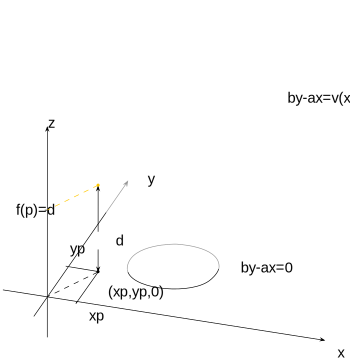
\includegraphics{figures/source/plot11}};


\path[draw=c989898,line join=round,line width=0.512pt] (173.2880,332.6840) -- (173.2970,290.3690);



\path[draw=c989898,line join=round,line width=0.512pt] (173.2970,288.2890) -- (173.3150,213.6110);



\path[draw=c989898,line join=round,line width=0.512pt] (173.3160,211.2310) -- (173.3390,113.4170);



\path[draw=black,line join=round,line width=0.512pt] (47.3201,297.3570) -- (324.8360,340.8940);



\path[draw=black,line join=round,line width=0.512pt] (47.3393,297.7850) -- (47.3804,127.3150);



\path[draw=black,line join=round,line width=0.512pt] (47.3257,337.8570) -- (47.3354,297.7680);



\path[draw=black,line join=round,line width=0.512pt] (47.2678,297.6320) -- (83.2534,245.9200);



\path[draw=black,line join=round,line width=0.512pt] (92.4553,232.6970) -- (105.4110,214.0800);



\path[draw=c989898,line join=round,line width=0.512pt] (107.5070,211.0670) -- (113.9760,201.7710);



\path[draw=c989898,line join=round,line width=0.512pt] (116.0050,198.8560) -- (127.7670,181.9540);



\path[fill=black,line join=round,line width=0.160pt] (45.1337,132.1130) -- (47.4067,130.1080) -- (49.4902,132.1040) -- (47.3042,126.3360) -- (45.1337,132.1130) -- cycle;



\path[fill=black,line join=round,line width=0.160pt] (320.4950,337.6730) -- (322.0070,340.2990) -- (319.6360,341.9440) -- (325.7240,340.9500) -- (320.4950,337.6730) -- cycle;



\path[cm={{1.0,0.0,0.0,1.0,(323.0,358.0)}}] (0.0000,0.0000) node[above right] () {$x$};



\path[cm={{1.0,0.0,0.0,1.0,(33.0,128.0)}}] (0.0000,0.0000) node[above right] () {$z$};



\path[cm={{1.0,0.0,0.0,1.0,(133.0,184.0)}}] (0.0000,0.0000) node[above right] () {$y$};



\path[draw=c989898,fill=c989898,line join=round,line width=0.160pt] (123.4090,184.7720) -- (126.3920,184.2350) -- (127.1390,187.0210) -- (128.2590,180.9550) -- (123.4090,184.7720) -- cycle;



\path[draw=black,line join=round,line width=0.512pt] (33.8411,316.9190) -- (47.2875,297.6020);



\path[draw=c989898,line join=round,line width=0.512pt] (219.3400,268.1300) .. controls (219.4020,267.7220) and (219.4350,267.3120) .. (219.4350,266.9020) .. controls (219.4350,246.0400) and (175.9680,244.5180) .. (175.9680,244.5180);



\path[draw=c989898,line join=round,line width=0.512pt] (170.9090,244.6550) .. controls (159.1350,245.2810) and (130.6670,248.6840) .. (127.5750,266.9020) .. controls (127.3910,267.9820) and (127.3660,269.0270) .. (127.4870,270.0360);



\path[draw=c989898,line join=round,line width=0.512pt] (127.4870,270.0360) .. controls (127.5930,270.9230) and (127.8120,271.7810) .. (128.1350,272.6120);



\path[draw=black,line join=round,line width=0.512pt] (128.1350,272.6120) .. controls (135.2830,291.0080) and (193.4860,295.5780) .. (210.9770,280.0880) .. controls (210.9770,280.0880) and (217.3970,275.0510) .. (219.0510,269.4220);



\path[draw=c989898,line join=round,line width=0.512pt] (219.0510,269.4220) .. controls (219.1760,268.9940) and (219.2750,268.5630) .. (219.3400,268.1300);

%here is the upper circle
\path[draw=black,line join=round,line width=0.512pt] (98.5146,184.9420) .. controls (110.1230,214.8150) and (204.6360,222.2350) .. (233.0370,197.0820) .. controls (233.0370,197.0820) and (243.4630,188.9020) .. (246.1480,179.7620);


\path[fill=foo,line join=round,line width=0.160pt] (84.9343,148.9700) -- (86.9687,145.2070) -- (90.8356,147.3020) -- (85.2988,139.7020) -- (84.9343,148.9700) -- cycle;



\path[draw=c989898,line join=round,line width=0.512pt] (246.1880,179.7470) .. controls (246.2880,179.0870) and (246.3410,178.4250) .. (246.3410,177.7630) .. controls (246.3410,144.0430) and (176.0870,141.5840) .. (176.0870,141.5840) .. controls (176.0870,141.5840) and (175.8910,141.5810) .. (175.5170,141.5810);



\path[draw=c989898,line join=round,line width=0.512pt] (171.7840,141.6430) .. controls (156.1870,142.1140) and (103.2510,146.0570) .. (97.8694,177.7630) .. controls (97.5732,179.5090) and (97.5329,181.1970) .. (97.7282,182.8280);



\path[fill=foo,line join=round,line width=0.160pt] (98.2177,183.9090) .. controls (99.0719,183.9090) and (99.7643,184.6020) .. (99.7643,185.4560) .. controls (99.7643,186.3100) and (99.0719,187.0030) .. (98.2177,187.0030) .. controls (97.3635,187.0030) and (96.6710,186.3100) .. (96.6710,185.4560) .. controls (96.6710,184.6020) and (97.3635,183.9090) .. (98.2177,183.9090) -- cycle;



\path[draw=black,line join=round,line width=0.512pt] (44.8080,210.4840) -- (47.5576,210.4910);



\path[cm={{1.0,0.0,0.0,1.0,(-10.0,215.0)}}] (0.0000,0.0000) node[above right] () {$\varphi(\mathbf{p})=d_2$};



\path[fill=foo,line join=round,line width=0.256pt] (88.6971,190.5360) -- (83.9057,192.8790) -- (83.6246,192.3040) -- (88.4160,189.9610) -- (88.6971,190.5360) -- cycle(79.1143,195.2210) -- (74.3230,197.5640) -- (74.0419,196.9890) -- (78.8333,194.6460) -- (79.1143,195.2210) -- cycle(69.5316,199.9060) -- (64.7402,202.2490) -- (64.4592,201.6740) -- (69.2505,199.3310) -- (69.5316,199.9060) -- cycle(59.9489,204.5910) -- (55.1575,206.9340) -- (54.8764,206.3590) -- (59.6678,204.0160) -- (59.9489,204.5910) -- cycle(50.3661,209.2760) -- (47.4761,210.6890) -- (47.1950,210.1140) -- (50.0851,208.7010) -- (50.3661,209.2760) -- cycle(98.2798,185.8510) -- (93.4884,188.1940) -- (93.2073,187.6190) -- (97.9987,185.2760) -- (98.2798,185.8510) -- cycle;



\path[cm={{1.0,0.0,0.0,1.0,(209.0,252.0)}}] (0.0000,0.0000) node[above right] () {$(x-3)^2+(y-3)^2-2=h$};



\path[draw=foo,fill=foo,line join=round,line width=0.160pt] (111.5160,222.6330) -- (109.6890,226.5640) -- (105.7670,224.5760) -- (111.5090,232.0200) -- (111.5160,222.6330) -- cycle;



\path[draw=foo,line join=round,line width=1.080pt] (98.2124,185.3970) -- (109.6740,227.0900);



\path[fill=foo,line join=round,line width=0.160pt] (173.2540,332.7580) .. controls (174.1080,332.7580) and (174.8000,333.4510) .. (174.8000,334.3050) .. controls (174.8000,335.1590) and (174.1080,335.8520) .. (173.2540,335.8520) .. controls (172.4000,335.8520) and (171.7070,335.1590) .. (171.7070,334.3050) .. controls (171.7070,333.4510) and (172.4000,332.7580) .. (173.2540,332.7580) -- cycle;



\path[cm={{1.0,0.0,0.0,1.0,(59.0,151.0)}}] (0.0000,0.0000) node[above right] () {$\nabla\varphi_i$};



\path[cm={{1.0,0.0,0.0,1.0,(78.0,247.0)}}] (0.0000,0.0000) node[above right] () {$-\nabla\varphi_i$};



\path[cm={{1.0,0.0,0.0,1.0,(161.0,351.0)}}] (0.0000,0.0000) node[above right] () {$\nabla\varphi_i=0$};



\path[fill=c989898,line join=round,line width=0.160pt] (173.3130,266.0410) .. controls (174.1670,266.0410) and (174.8590,266.7340) .. (174.8590,267.5880) .. controls (174.8590,268.4420) and (174.1670,269.1340) .. (173.3130,269.1340) .. controls (172.4580,269.1340) and (171.7660,268.4420) .. (171.7660,267.5880) .. controls (171.7660,266.7340) and (172.4580,266.0410) .. (173.3130,266.0410) -- cycle;



\path[fill=c989898,line join=round,line width=0.160pt] (173.2130,176.3380) .. controls (174.0670,176.3380) and (174.7590,177.0300) .. (174.7590,177.8840) .. controls (174.7590,178.7390) and (174.0670,179.4310) .. (173.2130,179.4310) .. controls (172.3590,179.4310) and (171.6660,178.7390) .. (171.6660,177.8840) .. controls (171.6660,177.0300) and (172.3590,176.3380) .. (173.2130,176.3380) -- cycle;



\path[draw=foo,line join=round,line width=1.080pt] (86.6208,143.8110) -- (98.0827,185.5040);




\end{tikzpicture}


  \caption[The direction of the gradient on a circle path function]{The direction of the gradient $\nabla\varphi_i$ in the point $(x_\mathbf{p},y_{\mathbf{p}})$ at an altitude $h$ w.r.t. $\mathcal{O}_W$ for the circle path function in \frefeq{eq:pathf-circle} and \fref{fig:circle-pf}{Figure}. The gradient directs where the function locally maximally increases; the opposite thus to the center of the circle in \frefeq{eq:two-paths} (or the base of the paraboloid $\varphi_i$).}
  \label{fig:grad}
\end{figure}
We note some analogies in the physical theory of potential functions with our path functions; indeed vector fields are a well-known concept in physics, with applications such as electrostatic\findex{electrostatic field}, gravitational\findex{gravitational field}, and magnetic fields\findex{magnetic field}~\citep{feynman2015feynman}. Imagine that the aerial robot is a positively charged particle in an electrostatics analysis, attracted by a negatively charged goal. Via the gradient, we can then direct the particle (the aerial robot) to the goal (where the function maximally locally decreases)~\citep{choset2005principles}. In the setting of \frefeq{eq:pathf-line} and \frefeq{eq:pathf-circle}, i.e., 
\begin{equation}\label{eq:two-paths}
  2y-x=h,\,\,\,\ (x-3)^2+(y-3)^2-2=h,
\end{equation}
their gradient then points away from the base of the plane in \frefeq{eq:pathf-line} and the center of the circle in \frefeq{eq:pathf-circle} in \fref{fig:grad}{Figure}. If the goal is not to fly over the circle in \fref{fig:circle-pf}{Figure}, but to its center $(x_c,y_c)$ in \frefeq{eq:pathf-circle}, the vector field $\varPhi$ in \frefeq{eq:vec-field-def} direct us in the opposite direction; we can then use $-\nabla\varphi_i$ to direct the robot to the goal.

Vector fields are common in the motion planning literature~\citep{choset2005principles,lavalle2006planning} and in studies~\citep{lindemann2005smoothly,gonccalves2010vector,panagou2014motion,zhou2014vector,kapitanyuk2017guiding,de2017guidance} for navigation and guidance of different mobile robots. A well-known intuitive method based on vector fields brought from optimization is the gradient descent algorithm\findex{gradient descent algorithm}~\citep{choset2005principles,bryson1975applied}, where an intuitive choice of the search direction is the negative gradient $\Delta \varphi_i:=-\nabla\varphi_i$~\citep{boyd2004convex}.
\begin{algorithm}[h!] %this is an example
  \SetKwInOut{Input}{Input}
  \SetKwInOut{Output}{Output}
  \SetKwFunction{FMain}{\small\tt zamboni-like\_motion}
  \SetKwProg{Fn}{Function}{:}{}
  \SetKwProg{Pn}{Function}{:}{\KwRet}

  \DontPrintSemicolon
  \Input{$t_0${ \otherfont initial time step}\newline
         $c^\rho_i${ \otherfont value of the path parameters}\newline
         $j${ \otherfont current stage}
  }
  \Output{$\mathbf{p}(\mathcal{K})${ \otherfont trajectory}
  }
  \vspace{.8ex}

  \ForEach{\normalsize $i\in\mathcal{K}:=\{t_0,t_0+h,t_0+2h,\dots\}$}{
    \If{\normalsize $\norm{\nabla\varphi_j(\mathbf{p}(t),c^\rho_i)}\leq \varepsilon$}{
      \vspace{.8ex}
      \Return{\normalsize $\mathbf{p}(\mathcal{K})$}\;
    }
    {\normalsize $\mathbf{p}(i+h)\gets \mathbf{p}(i)+\theta(i)\Delta\varphi_j(\mathbf{p}(t),c^\rho_i)$}\;
  }
  \vspace{1.6ex}

  \caption{Gradient descent}\findex{gradient descent}
  \label{algo:grad-desc}
\end{algorithm}
We detail the gradient descent algorithm in \fref{algo:grad-desc}{Algorithm}, where we iterate at discrete time steps, meaning that at instant $n$, $\mathcal{K}$ contains $t_0,t_0+h,\dots,t_0+nh$. We discuss further the time step $h$ ($h$is not to be confused with the altitude when used in the path functions) later in this chapter in \fref{sec:algo}{Section}. In the algorithm, $\mathbf{p}(t_0)$ is given (e.g., from sensors data), $\theta(i)$ is a scalar step size at time instant $i$~\citep{choset2005principles}--there can be indeed different step sizes at different instants--and $\varepsilon\in\mathbb{R}_{>0}$ is chosen based on the task requirements (it is unrealistic to assume we will reach $\nabla\varphi_i=0$).

We discuss in the next section how to fix $\varPhi$ so that it directs us to follow \frefeq{eq:two-paths} rather than, e.g., to $\nabla\varphi_i=0$.

\subsection{Derivation of a path following vector field}

\fref{algo:grad-desc}{Algorithm} that we illustrate in \fref{fig:grad_desc}{Figure} directs to the center of the circle when we have a circle as a path function in \frefeq{eq:two-paths}.
\begin{figure}[h!]
  \centering
  \fontfamily{phv}\selectfont
  
\definecolor{c989898}{RGB}{152,152,152}
\small

\def \globalscale {1.000000}
\begin{tikzpicture}[y=0.80pt, x=0.80pt, yscale=-\globalscale, xscale=\globalscale, inner sep=0pt, outer sep=0pt]
\path[draw=black,line join=round,line width=0.512pt] (10.4871,206.0790) -- (222.2210,206.0800);



\path[draw=black,line join=round,line width=0.512pt] (16.1042,10.3269) -- (16.1041,128.8180);



\path[draw=black,line join=round,line width=0.512pt] (16.1041,148.0200) -- (16.1041,212.0610);



\path[fill=black,line join=round,line width=0.160pt] (14.1422,14.1208) -- (16.1124,12.3829) -- (17.9183,14.1129) -- (16.0235,9.1129) -- (14.1422,14.1208) -- cycle;



\path[fill=black,line join=round,line width=0.160pt] (220.0700,204.0730) -- (221.8080,206.0430) -- (220.0780,207.8490) -- (225.0780,205.9540) -- (220.0700,204.0730) -- cycle;



\path[draw=c989898,line join=round,line width=0.512pt] (149.8410,78.8284) .. controls (154.3410,84.7637) and (157.0120,92.1629) .. (157.0120,100.1860) .. controls (157.0120,119.7270) and (141.1700,135.5680) .. (121.6290,135.5680) .. controls (102.0880,135.5680) and (86.2470,119.7270) .. (86.2470,100.1860) .. controls (86.2470,80.6446) and (102.0880,64.8033) .. (121.6290,64.8033) .. controls (129.8280,64.8033) and (137.3750,67.5916) .. (143.3740,72.2717);



\path[draw=c989898,line join=round,line width=0.512pt] (182.5090,96.6832) .. controls (182.5660,97.7650) and (182.5950,98.8543) .. (182.5950,99.9503) .. controls (182.5950,133.6210) and (155.2990,160.9160) .. (121.6290,160.9160) .. controls (87.9590,160.9160) and (60.6638,133.6210) .. (60.6638,99.9503) .. controls (60.6638,66.2801) and (87.9590,38.9848) .. (121.6290,38.9848) .. controls (150.9150,38.9848) and (175.3790,59.6349) .. (181.2530,87.1686);



\path[draw=c989898,line join=round,line width=0.512pt] (145.1750,24.6380) .. controls (177.2720,34.6552) and (200.5690,64.6102) .. (200.5690,100.0060) .. controls (200.5690,143.6030) and (165.2260,178.9460) .. (121.6290,178.9460) .. controls (78.0322,178.9460) and (42.6898,143.6030) .. (42.6898,100.0060) .. controls (42.6898,56.4095) and (78.0322,21.0669) .. (121.6290,21.0669) .. controls (125.2030,21.0669) and (128.7210,21.3043) .. (132.1690,21.7643);



\path[draw=black,line join=round,line width=0.512pt] (169.1290,84.0395) .. controls (170.8430,89.0955) and (171.7730,94.5140) .. (171.7730,100.1490) .. controls (171.7730,127.8430) and (149.3230,150.2930) .. (121.6290,150.2930) .. controls (93.9356,150.2930) and (71.4855,127.8430) .. (71.4855,100.1490) .. controls (71.4855,72.4559) and (93.9356,50.0056) .. (121.6290,50.0056) .. controls (140.6690,50.0056) and (157.2300,60.6169) .. (165.7210,76.2480);



\path[draw=c989898,line join=round,line width=0.512pt] (123.3230,13.4268) .. controls (170.3700,14.3427) and (208.2270,52.7672) .. (208.2270,100.0330) .. controls (208.2270,147.8740) and (169.4450,186.6560) .. (121.6040,186.6560) .. controls (73.7637,186.6560) and (34.9813,147.8740) .. (34.9813,100.0330) .. controls (34.9813,56.4761) and (67.1302,20.4270) .. (108.9940,14.3212);



\path[draw=c989898,line join=round,line width=0.512pt] (158.4340,39.8940) .. controls (178.6100,52.2827) and (192.0660,74.5505) .. (192.0660,99.9615) .. controls (192.0660,138.8630) and (160.5300,170.3980) .. (121.6290,170.3980) .. controls (82.7282,170.3980) and (51.1927,138.8630) .. (51.1927,99.9615) .. controls (51.1927,61.0606) and (82.7282,29.5249) .. (121.6290,29.5249) .. controls (130.9120,29.5249) and (139.7750,31.3205) .. (147.8900,34.5835);



\path[fill=foo,line join=round,line width=0.160pt] (121.4980,98.8207) .. controls (122.2380,98.8207) and (122.8380,99.4209) .. (122.8380,100.1610) .. controls (122.8380,100.9020) and (122.2380,101.5020) .. (121.4980,101.5020) .. controls (120.7570,101.5020) and (120.1570,100.9020) .. (120.1570,100.1610) .. controls (120.1570,99.4209) and (120.7570,98.8207) .. (121.4980,98.8207) -- cycle;



\path[fill=foo,line join=round,line width=0.160pt] (50.9590,135.0120) ellipse (0.0378cm and 0.0378cm);



\path[draw=foo,line join=round,line width=0.512pt] (51.0193,135.0320) -- (58.2991,131.4430);



\path[fill=foo,line join=round,line width=0.256pt] (63.0120,128.9410) -- (65.4039,127.7620) -- (65.5453,128.0490) -- (63.1535,129.2280) -- (63.0120,128.9410) -- cycle(67.7957,126.5830) -- (70.1875,125.4040) -- (70.3290,125.6910) -- (67.9372,126.8700) -- (67.7957,126.5830) -- cycle(72.5794,124.2250) -- (74.9712,123.0460) -- (75.1127,123.3330) -- (72.7209,124.5120) -- (72.5794,124.2250) -- cycle(77.3631,121.8670) -- (79.7549,120.6880) -- (79.8964,120.9750) -- (77.5045,122.1540) -- (77.3631,121.8670) -- cycle(82.1467,119.5090) -- (84.5386,118.3300) -- (84.6801,118.6170) -- (82.2882,119.7960) -- (82.1467,119.5090) -- cycle(86.9304,117.1510) -- (89.3222,115.9720) -- (89.4637,116.2590) -- (87.0719,117.4380) -- (86.9304,117.1510) -- cycle(91.7141,114.7930) -- (94.1059,113.6130) -- (94.2474,113.9010) -- (91.8556,115.0800) -- (91.7141,114.7930) -- cycle(96.4978,112.4340) -- (98.8896,111.2550) -- (99.0311,111.5420) -- (96.6393,112.7210) -- (96.4978,112.4340) -- cycle(101.2810,110.0760) -- (103.6730,108.8970) -- (103.8150,109.1840) -- (101.4230,110.3630) -- (101.2810,110.0760) -- cycle(106.0650,107.7180) -- (108.4570,106.5390) -- (108.5980,106.8260) -- (106.2070,108.0050) -- (106.0650,107.7180) -- cycle(110.8490,105.3600) -- (113.2410,104.1810) -- (113.3820,104.4680) -- (110.9900,105.6470) -- (110.8490,105.3600) -- cycle(115.6320,103.0020) -- (118.0240,101.8230) -- (118.1660,102.1100) -- (115.7740,103.2890) -- (115.6320,103.0020) -- cycle(120.4160,100.6440) -- (121.6180,100.0510) -- (121.7600,100.3380) -- (120.5580,100.9310) -- (120.4160,100.6440) -- cycle(58.2284,131.3000) -- (60.6202,130.1210) -- (60.7617,130.4080) -- (58.3698,131.5870) -- (58.2284,131.3000) -- cycle;



\path[fill=foo,line join=round,line width=0.160pt] (58.4502,131.3860) ellipse (0.0378cm and 0.0378cm);



\path[fill=foo,line join=round,line width=0.160pt] (66.9795,125.6080) .. controls (67.7198,125.6080) and (68.3201,126.2080) .. (68.3201,126.9480) .. controls (68.3201,127.6890) and (67.7198,128.2890) .. (66.9795,128.2890) .. controls (66.2390,128.2890) and (65.6388,127.6890) .. (65.6388,126.9480) .. controls (65.6388,126.2080) and (66.2390,125.6080) .. (66.9795,125.6080) -- cycle;



\path[fill=foo,line join=round,line width=0.160pt] (76.6875,120.9270) .. controls (77.4279,120.9270) and (78.0281,121.5270) .. (78.0281,122.2680) .. controls (78.0281,123.0080) and (77.4279,123.6080) .. (76.6875,123.6080) .. controls (75.9471,123.6080) and (75.3468,123.0080) .. (75.3468,122.2680) .. controls (75.3468,121.5270) and (75.9471,120.9270) .. (76.6875,120.9270) -- cycle;



\path[fill=foo,line join=round,line width=0.160pt] (89.7933,114.2820) .. controls (90.5337,114.2820) and (91.1339,114.8820) .. (91.1339,115.6220) .. controls (91.1339,116.3630) and (90.5337,116.9630) .. (89.7933,116.9630) .. controls (89.0529,116.9630) and (88.4527,116.3630) .. (88.4527,115.6220) .. controls (88.4527,114.8820) and (89.0529,114.2820) .. (89.7933,114.2820) -- cycle;



\path[cm={{1.0,0.0,0.0,1.0,(166.0,82.0)}}] (0.0000,0.0000) node[above right] () {\scriptsize $h$};



\path[cm={{1.0,0.0,0.0,1.0,(141.0,78.0)}}] (0.0000,0.0000) node[above right] () {\scriptsize -1};



\path[cm={{1.0,0.0,0.0,1.0,(175.0,95.0)}}] (0.0000,0.0000) node[above right] () {\scriptsize +1};



\path[cm={{1.0,0.0,0.0,1.0,(146.0,41.0)}}] (0.0000,0.0000) node[above right] () {\scriptsize +2};



\path[cm={{1.0,0.0,0.0,1.0,(133.0,27.0)}}] (0.0000,0.0000) node[above right] () {\scriptsize +3};



\path[cm={{1.0,0.0,0.0,1.0,(110.0,16.0)}}] (0.0000,0.0000) node[above right] () {\scriptsize +4};



\path[cm={{1.0,0.0,0.0,1.0,(222.0,222.0)}}] (0.0000,0.0000) node[above right] () {$x$};



\path[cm={{1.0,0.0,0.0,1.0,(0.0,7.0)}}] (0.0000,0.0000) node[above right] () {$y$};



\path[cm={{1.0,0.0,0.0,1.0,(110.0,119.0)}}] (0.0000,0.0000) node[above right] () {$\nabla\varphi_i=0$};



\path[cm={{1.0,0.0,0.0,1.0,(42.0,196.0)}}] (0.0000,0.0000) node[above right] () {$\mathbf{p}(t_0+h)$};



\path[draw=black,line join=round,line width=0.512pt] (51.6569,181.8440) .. controls (51.6569,181.8440) and (43.5503,166.9640) .. (48.7769,158.0040) .. controls (54.0036,149.0440) and (57.4702,146.6280) .. (58.6435,135.1080);



\path[cm={{1.0,0.0,0.0,1.0,(1.0,143.5)}}] (0.0000,0.0000) node[above right] () {$\mathbf{p}(t_0)$};



\path[draw=black,line join=round,line width=0.512pt] (24.5102,135.5880) .. controls (24.5102,135.5880) and (27.5769,136.2540) .. (35.3635,134.2280) .. controls (40.6100,132.8620) and (41.7368,130.6280) .. (47.3369,133.0810);




\end{tikzpicture}


  \caption[The gradient descent algorithm illustrated on a circle path function]{The gradient descent algorithm after the first two steps, with the following step being dashed and directing the aerial robot to the center of the circle where the gradient is zero $\nabla\varphi_i=0$. The paraboloid $\varphi_i$ representing the path function circle at altitude $h$ is illustrated in the contour plot.}
  \label{fig:grad_desc}
\end{figure}
However, we want to track (or follow) these functions. Concretely, in the path sub-plan in \frefeqM{eq:line-gene}{eq:circ-gene} in \fref{sec:path-wise}{Section}, we want to follow the path function $\varphi_{i+1}$ by flying over rather than heading the center when we follow a circle path function. In the example, we started following the circle described by $\varphi_{i+1}$ after reaching $\mathbf{p}_{\Gamma_i}$ while tracking $\varphi_i$ (for all the previous and following path functions). To this end, we use a vector field-based approach proposed in the literature specifically for aerial robots~\citep{de2017guidance}, which points to the contours of the functions in \fref{fig:line-pf}{Figures}\fref{fig:circle-pf}{--\hspace{-.8ex}} and thus to \frefeq{eq:two-paths}.

The expression for the search direction $\Delta\varphi_i$ in \fref{algo:grad-desc}{Algorithm} using the vector field in~\citep{de2017guidance} becomes
\begin{equation}\label{eq:pd}
  \Delta_d\varphi_i(\mathbf{p}(t),c_i^\rho):=E_i\nabla\varphi_i(\mathbf{p}(t),c_i^\rho)-k_e\varphi_i(\mathbf{p}(t),c_i^\rho)\nabla\varphi_i(\mathbf{p}(t),c_i^\rho),
\end{equation}
where $E_i\nabla\varphi_i(\mathbf{p}(t),c_i^\rho)$ is a vector pointing perpendicularly to the gradient $\nabla\varphi_i(\mathbf{p}(t),c_i^\rho)$, $E_i$ is the $i$th stage direction
\begin{equation}
  E_i=\begin{bmatrix}
    0&1\\-1&0
  \end{bmatrix},
\end{equation}
with $E_i$ being the counterclockwise, $-E_i$ the clockwise direction. 
The contribution of the component $-k_e\varphi_i(\mathbf{p}(t),c_i^\rho)\nabla\varphi_i(\mathbf{p}(t),c_i^\rho)$ in \frefeq{eq:pd} points in the direction of the path function. It depends on the coefficient $k_e\in\mathbb{R}_{>0}$--indicating the speed of convergence~\citep{de2017guidance}--and on the value of $\varphi_i$ at the current point (of course also on the path parameters and the value of the gradient). 
\begin{figure}[h!]
  \centering
  \fontfamily{phv}\selectfont
  
\definecolor{c989898}{RGB}{152,152,152}
\small

\def \globalscale {1.000000}
\begin{tikzpicture}[y=0.80pt, x=0.80pt, yscale=-\globalscale, xscale=\globalscale, inner sep=0pt, outer sep=0pt]
\path[draw=black,line join=round,line width=0.512pt] (10.4871,206.0790) -- (222.2210,206.0800);



\path[fill=black,line join=round,line width=0.160pt] (14.1422,14.1208) -- (16.1123,12.3830) -- (17.9183,14.1129) -- (16.0235,9.1130) -- (14.1422,14.1208) -- cycle;



\path[fill=black,line join=round,line width=0.160pt] (220.0700,204.0730) -- (221.8080,206.0430) -- (220.0780,207.8490) -- (225.0780,205.9540) -- (220.0700,204.0730) -- cycle;



\path[draw=c989898,line join=round,line width=0.512pt] (133.8120,133.4070) .. controls (126.8210,135.9760) and (118.9640,136.3680) .. (111.2910,134.0240) .. controls (94.7687,128.9760) and (84.6296,112.9310) .. (86.4473,96.3651);



\path[draw=c989898,line join=round,line width=0.512pt] (90.4009,83.5370) .. controls (92.4400,79.7024) and (95.1311,76.3528) .. (98.2612,73.5481) .. controls (98.2612,73.5481) and (98.0851,73.3709) .. (101.9080,70.8080) .. controls (105.7300,68.2450) and (110.0370,66.4338) .. (114.5780,65.5062);



\path[draw=c989898,line join=round,line width=0.512pt] (126.5880,65.1474) .. controls (128.3820,65.4036) and (130.1800,65.8012) .. (131.9670,66.3473) .. controls (141.0700,69.1283) and (148.2350,75.2473) .. (152.5310,82.9524);



\path[draw=c989898,line join=round,line width=0.512pt] (156.3180,93.1815) .. controls (157.4500,98.7616) and (157.2480,104.6950) .. (155.4680,110.5230) .. controls (153.0720,118.3640) and (148.2010,124.7670) .. (141.9720,129.1370);



\path[draw=c989898,line join=round,line width=0.512pt] (182.5090,96.6833) .. controls (182.5660,97.7651) and (182.5950,98.8544) .. (182.5950,99.9504) .. controls (182.5950,133.6210) and (155.2990,160.9160) .. (121.6290,160.9160) .. controls (87.9590,160.9160) and (60.6638,133.6210) .. (60.6638,99.9504) .. controls (60.6638,97.1165) and (60.8572,94.3277) .. (61.2314,91.5964);



\path[draw=c989898,line join=round,line width=0.512pt] (62.3203,85.7757) .. controls (68.7099,58.9414) and (92.8391,38.9850) .. (121.6290,38.9850) .. controls (150.9150,38.9850) and (175.3790,59.6350) .. (181.2530,87.1687);



\path[draw=c989898,line join=round,line width=0.512pt] (145.1750,24.6381) .. controls (177.2720,34.6552) and (200.5690,64.6103) .. (200.5690,100.0060) .. controls (200.5690,143.6040) and (165.2260,178.9460) .. (121.6290,178.9460) .. controls (78.0322,178.9460) and (42.6897,143.6040) .. (42.6897,100.0060) .. controls (42.6897,56.4095) and (78.0322,21.0669) .. (121.6290,21.0669) .. controls (125.2030,21.0669) and (128.7210,21.3044) .. (132.1690,21.7643);



\path[draw=black,line join=round,line width=0.512pt] (169.1290,84.0395) .. controls (170.8430,89.0956) and (171.7730,94.5141) .. (171.7730,100.1490) .. controls (171.7730,127.8430) and (149.3230,150.2930) .. (121.6290,150.2930) .. controls (93.9357,150.2930) and (71.4855,127.8430) .. (71.4855,100.1490) .. controls (71.4855,98.8747) and (71.5331,97.6111) .. (71.6266,96.3603);



\path[draw=black,line join=round,line width=0.512pt] (74.5660,82.8058) .. controls (75.9064,79.1698) and (77.6561,75.7318) .. (79.7593,72.5478) .. controls (84.9888,64.6310) and (90.0729,60.9404) .. (90.0729,60.9404) .. controls (97.9571,54.8733) and (107.3890,50.9579) .. (117.6940,50.1579) .. controls (128.0000,49.3579) and (134.5790,51.7028) .. (134.5790,51.7028) .. controls (147.9560,55.2295) and (159.2100,64.2632) .. (165.7210,76.2481);



\path[draw=c989898,line join=round,line width=0.512pt] (123.3230,13.4268) .. controls (170.3700,14.3428) and (208.2270,52.7672) .. (208.2270,100.0330) .. controls (208.2270,147.8740) and (169.4450,186.6560) .. (121.6040,186.6560) .. controls (73.7637,186.6560) and (34.9812,147.8740) .. (34.9812,100.0330) .. controls (34.9812,56.4762) and (67.1302,20.4271) .. (108.9940,14.3213);



\path[draw=c989898,line join=round,line width=0.512pt] (158.4340,39.8940) .. controls (178.6100,52.2827) and (192.0660,74.5505) .. (192.0660,99.9615) .. controls (192.0660,138.8630) and (160.5300,170.3980) .. (121.6290,170.3980) .. controls (82.7282,170.3980) and (51.1927,138.8630) .. (51.1927,99.9615) .. controls (51.1927,61.0606) and (82.7282,29.5250) .. (121.6290,29.5250) .. controls (130.9120,29.5250) and (139.7750,31.3205) .. (147.8900,34.5835);



\path[cm={{1.0,0.0,0.0,1.0,(165.0,82.0)}}] (0.0000,0.0000) node[above right] () {\footnotesize $h$};



\path[cm={{1.0,0.0,0.0,1.0,(134.0,134.0)}}] (0.0000,0.0000) node[above right] () {\scriptsize -1};



\path[cm={{1.0,0.0,0.0,1.0,(175.0,95.0)}}] (0.0000,0.0000) node[above right] () {\scriptsize +1};



\path[cm={{1.0,0.0,0.0,1.0,(146.0,41.0)}}] (0.0000,0.0000) node[above right] () {\scriptsize +2};



\path[cm={{1.0,0.0,0.0,1.0,(133.0,27.0)}}] (0.0000,0.0000) node[above right] () {\scriptsize +3};



\path[cm={{1.0,0.0,0.0,1.0,(110.0,16.0)}}] (0.0000,0.0000) node[above right] () {\scriptsize +4};



\path[cm={{1.0,0.0,0.0,1.0,(222.0,222.0)}}] (0.0000,0.0000) node[above right] () {$x$};



\path[cm={{1.0,0.0,0.0,1.0,(0.0,7.0)}}] (0.0000,0.0000) node[above right] () {$y$};



\path[cm={{1.0,0.0,0.0,1.0,(115.0,111.0)}}] (0.0000,0.0000) node[above right] () {$\mathbf{p}_{-}$};



\path[draw=black,line join=round,line width=0.512pt] (16.1205,212.0240) -- (16.1207,12.0904);



\path[fill=foo,line join=round,line width=0.160pt] (117.4910,94.7552) .. controls (118.3230,94.7552) and (118.9980,95.4296) .. (118.9980,96.2615) .. controls (118.9980,97.0935) and (118.3230,97.7679) .. (117.4910,97.7679) .. controls (116.6590,97.7679) and (115.9850,97.0935) .. (115.9850,96.2615) .. controls (115.9850,95.4296) and (116.6590,94.7552) .. (117.4910,94.7552) -- cycle;



\path[draw=foo,line join=round,line width=0.512pt] (137.1290,81.0573) -- (117.4770,96.3559);



\path[fill=foo,line join=round,line width=0.160pt] (132.5460,82.2033) -- (134.8070,82.7863) -- (134.7800,84.9021) -- (137.5090,80.7032) -- (132.5460,82.2033) -- cycle;



\path[fill=foo,line join=round,line width=0.160pt] (103.3310,81.1697) -- (103.9140,78.9085) -- (106.0290,78.9362) -- (101.8300,76.2069) -- (103.3310,81.1697) -- cycle;



\path[draw=foo,line join=round,line width=1.024pt] (117.5090,96.1708) -- (121.4550,65.2660);



\path[fill=foo,line join=round,line width=0.160pt] (118.8210,67.4179) -- (121.3800,65.7285) -- (123.5160,67.9344) -- (121.7790,61.5687) -- (118.8210,67.4179) -- cycle;



\path[cm={{1.0,0.0,0.0,1.0,(57.0,95.0)}}] (0.0000,0.0000) node[above right] () {$-k_e\varphi_i\nabla\varphi_i$};



\path[cm={{1.0,0.0,0.0,1.0,(118.0,62.5)}}] (0.0000,0.0000) node[above right] () {$\Delta_d\varphi_i$};



\path[cm={{1.0,0.0,0.0,1.0,(135.5,94.0)}}] (0.0000,0.0000) node[above right] () {$E_i\nabla\varphi_i$};



\path[draw=foo,line join=round,line width=0.512pt] (102.2260,76.7467) -- (117.5240,96.3985);



\path[fill=foo,line join=round,line width=0.256pt] (125.2350,65.5418) -- (126.8730,67.6461) -- (126.6210,67.8426) -- (124.9830,65.7384) -- (125.2350,65.5418) -- cycle(128.5110,69.7503) -- (130.1500,71.8545) -- (129.8970,72.0510) -- (128.2590,69.9468) -- (128.5110,69.7503) -- cycle(131.7880,73.9587) -- (133.4260,76.0630) -- (133.1730,76.2595) -- (131.5350,74.1552) -- (131.7880,73.9587) -- cycle(135.0640,78.1671) -- (136.7020,80.2713) -- (136.4490,80.4679) -- (134.8110,78.3637) -- (135.0640,78.1671) -- cycle(121.9590,61.3334) -- (123.5970,63.4376) -- (123.3450,63.6341) -- (121.7060,61.5299) -- (121.9590,61.3334) -- cycle;



\path[fill=foo,line join=round,line width=0.256pt] (117.7320,64.8363) -- (115.6280,66.4744) -- (115.4320,66.2219) -- (117.5360,64.5838) -- (117.7320,64.8363) -- cycle(113.5240,68.1125) -- (111.4200,69.7506) -- (111.2230,69.4981) -- (113.3270,67.8600) -- (113.5240,68.1125) -- cycle(109.3160,71.3887) -- (107.2110,73.0268) -- (107.0150,72.7743) -- (109.1190,71.1362) -- (109.3160,71.3887) -- cycle(105.1070,74.6649) -- (103.0030,76.3030) -- (102.8060,76.0505) -- (104.9110,74.4124) -- (105.1070,74.6649) -- cycle(121.9410,61.5601) -- (119.8370,63.1982) -- (119.6400,62.9456) -- (121.7440,61.3076) -- (121.9410,61.5601) -- cycle;




\end{tikzpicture}


  \caption[The direction of the vector field inside the path function]{The direction of the vector field for guidance in~\citep{de2017guidance} with a point $\mathbf{p}_{-}$ inside the circle: $\Delta_d$ points to the path function opposite to the center of the circle.}
  \label{fig:grad_gvf1}
\end{figure}
We illustrate $\Delta_d\varphi_i$ in \fref{fig:grad_gvf1}{Figure}. When we take a point within the circle, let's call it $\mathbf{p}_{-}$, the value of $\varphi_i$ is negative; $-k_e\varphi_i(\mathbf{p}_{-},c_i^\rho)\nabla\varphi_i(\mathbf{p}_{-},c_i^\rho)$ points outwards of the circle center, in the direction of the path function. $E_i\nabla\varphi_i(\mathbf{p}_{-},c_i^\rho)$ points perpendicularly to the gradient $\nabla\varphi_i$ and to the path function itself. The resulting vector $\Delta_d\varphi_i(\mathbf{p}_{-},c_i^\rho)$ then points to the direction of the path function.

Now we take a point $\mathbf{p}_{+}$ out of the circle, and not exactly over the path function. 
\begin{figure}[h!]
  \centering
  \fontfamily{phv}\selectfont
  
\definecolor{c989898}{RGB}{152,152,152}
\small

\def \globalscale {1.000000}
\begin{tikzpicture}[y=0.80pt, x=0.80pt, yscale=-\globalscale, xscale=\globalscale, inner sep=0pt, outer sep=0pt]
\path[draw=black,line join=round,line width=0.512pt] (10.4871,211.7520) -- (222.2210,211.7520);



\path[fill=black,line join=round,line width=0.160pt] (14.1422,19.7934) -- (16.1124,18.0556) -- (17.9183,19.7855) -- (16.0235,14.7856) -- (14.1422,19.7934) -- cycle;



\path[fill=black,line join=round,line width=0.160pt] (220.0700,209.7460) -- (221.8080,211.7160) -- (220.0780,213.5220) -- (225.0780,211.6270) -- (220.0700,209.7460) -- cycle;



\path[draw=c989898,line join=round,line width=0.512pt] (156.9830,107.3350) .. controls (156.6770,114.7780) and (154.0290,122.1850) .. (148.9230,128.3730) .. controls (136.4890,143.4480) and (114.1880,145.5870) .. (99.1141,133.1530) .. controls (93.1218,128.2090) and (89.1734,121.7070) .. (87.3720,114.7200);



\path[draw=c989898,line join=round,line width=0.512pt] (86.3900,102.6420) .. controls (87.0090,95.7918) and (89.6277,89.0497) .. (94.3350,83.3432) .. controls (106.7700,68.2690) and (129.0700,66.1292) .. (144.1440,78.5640) .. controls (150.4690,83.7808) and (154.5160,90.7343) .. (156.1660,98.1620);



\path[draw=c989898,line join=round,line width=0.512pt] (137.8470,164.5090) .. controls (136.8020,164.7950) and (135.7440,165.0550) .. (134.6730,165.2880) .. controls (101.7740,172.4540) and (69.2954,151.5930) .. (62.1298,118.6940) .. controls (61.8101,117.2260) and (61.5462,115.7590) .. (61.3366,114.2950);



\path[draw=c989898,line join=round,line width=0.512pt] (61.1317,98.6164) .. controls (61.8346,92.6187) and (63.4247,86.8200) .. (65.7934,81.3897);



\path[draw=c989898,line join=round,line width=0.512pt] (70.1766,73.1268) .. controls (78.5934,59.8229) and (92.1270,49.7654) .. (108.7240,46.1505) .. controls (141.6230,38.9848) and (174.1020,59.8458) .. (181.2680,92.7447) .. controls (187.5000,121.3600) and (172.5290,149.6580) .. (146.8760,161.2570);



\path[draw=c989898,line join=round,line width=0.512pt] (200.2970,112.6980) .. controls (197.3400,146.1910) and (173.0290,175.3290) .. (138.4430,182.8620) .. controls (95.8451,192.1410) and (53.7908,165.1290) .. (44.5126,122.5310) .. controls (40.6817,104.9420) and (43.0375,87.4462) .. (50.1228,72.3118);



\path[draw=c989898,line join=round,line width=0.512pt] (55.5210,62.6127) .. controls (66.4560,45.8421) and (83.7365,33.1974) .. (104.8440,28.6000) .. controls (147.4420,19.3218) and (189.4970,46.3332) .. (198.7750,88.9315) .. controls (199.5360,92.4232) and (200.0520,95.9114) .. (200.3370,99.3781);



\path[draw=black,line join=round,line width=0.512pt] (168.5180,121.8690) .. controls (166.7810,126.9170) and (164.2020,131.7720) .. (160.7540,136.2300) .. controls (143.8120,158.1370) and (112.3190,162.1610) .. (90.4124,145.2190) .. controls (80.2746,137.3790) and (73.9664,126.4220) .. (71.7936,114.7410);



\path[draw=black,line join=round,line width=0.512pt] (71.0292,102.5700) .. controls (71.3806,96.5828) and (72.8062,90.6199) .. (75.3447,84.9863);



\path[draw=black,line join=round,line width=0.512pt] (83.3591,72.5229) .. controls (94.1790,60.1404) and (109.9430,54.2719) .. (125.3950,55.5891);



\path[draw=black,line join=round,line width=0.512pt] (149.9440,64.5434) .. controls (150.5580,64.9759) and (151.1650,65.4241) .. (151.7650,65.8881) .. controls (166.8260,77.5358) and (173.4350,96.0612) .. (170.5890,113.6210);



\path[draw=c989898,line join=round,line width=0.512pt] (206.6000,88.9608) .. controls (215.7180,135.1250) and (186.2300,180.2920) .. (140.0470,190.3510) .. controls (93.3025,200.5320) and (47.1549,170.8920) .. (36.9736,124.1470) .. controls (32.9512,105.6800) and (35.1445,87.3051) .. (42.1524,71.2048);



\path[draw=c989898,line join=round,line width=0.512pt] (46.8692,61.9277) .. controls (58.6804,41.7773) and (78.5562,26.4365) .. (103.1770,21.0739) .. controls (145.7370,11.8041) and (187.8020,35.5447) .. (202.6770,75.1498);



\path[draw=c989898,line join=round,line width=0.512pt] (188.2120,128.9000) .. controls (180.4010,151.2500) and (161.5070,169.1370) .. (136.6780,174.5450) .. controls (98.6678,182.8230) and (61.1433,158.7220) .. (52.8645,120.7120) .. controls (51.4058,114.0140) and (50.9525,107.3320) .. (51.4031,100.8220);



\path[draw=c989898,line join=round,line width=0.512pt] (51.7229,97.4178) .. controls (51.9380,95.6052) and (52.2231,93.8083) .. (52.5762,92.0308);



\path[draw=c989898,line join=round,line width=0.512pt] (53.8645,86.6616) .. controls (60.7017,62.4116) and (80.3612,42.6348) .. (106.6970,36.8986) .. controls (144.7070,28.6199) and (182.2320,52.7216) .. (190.5110,90.7314) .. controls (192.4860,99.8014) and (192.6180,108.8440) .. (191.1570,117.4680);



\path[cm={{1.0,0.0,-0.0,1.0,(166.0,121.0)}}] (0.0000,0.0000) node[above right] () {\footnotesize $h$};



\path[cm={{1.0,0.0,0.0,1.0,(152.0,105.0)}}] (0.0000,0.0000) node[above right] () {\scriptsize -1};



\path[cm={{1.0,0.0,0.0,1.0,(137.0,165.0)}}] (0.0000,0.0000) node[above right] () {\scriptsize +1};



\path[cm={{1.0,0.0,0.0,1.0,(183.0,127.0)}}] (0.0000,0.0000) node[above right] () {\scriptsize +2};



\path[cm={{1.0,0.0,0.0,1.0,(194.0,109.0)}}] (0.0000,0.0000) node[above right] () {\scriptsize +3};



\path[cm={{1.0,0.0,0.0,1.0,(198.0,84.0)}}] (0.0000,0.0000) node[above right] () {\scriptsize +4};



\path[cm={{1.0,0.0,0.0,1.0,(222.0,227.0)}}] (0.0000,0.0000) node[above right] () {$x$};



\path[cm={{1.0,0.0,0.0,1.0,(0.0,13.0)}}] (0.0000,0.0000) node[above right] () {$y$};



\path[draw=black,line join=round,line width=0.512pt] (16.1484,217.7690) -- (16.1483,134.0760);



\path[draw=black,line join=round,line width=0.512pt] (16.1485,120.1690) -- (16.1486,17.8353);



\path[fill=foo,line join=round,line width=0.160pt] (104.1070,57.3859) .. controls (104.7650,57.8948) and (104.8860,58.8409) .. (104.3770,59.4990) .. controls (103.8680,60.1571) and (102.9220,60.2780) .. (102.2640,59.7690) .. controls (101.6060,59.2601) and (101.4850,58.3140) .. (101.9940,57.6559) .. controls (102.5030,56.9978) and (103.4490,56.8769) .. (104.1070,57.3859) -- cycle;



\path[cm={{1.0,-0.0,0.0,1.0,(124.0,64.0)}}] (0.0000,0.0000) node[above right] () {$E_i\nabla\varphi_i$};



\path[draw=foo,line join=round,line width=1.024pt] (103.5670,58.5972) -- (126.2760,49.9152);



\path[fill=foo,line join=round,line width=0.160pt] (122.2410,48.9168) -- (124.9530,50.3465) -- (124.0480,53.2806) -- (128.7920,48.6945) -- (122.2410,48.9168) -- cycle;



  \path[fill=foo,line join=round,line width=0.160pt] (43.7717,96.9146) .. controls (44.3759,97.4865) and (44.4022,98.4398) .. (43.8303,99.0441) .. controls (43.2585,99.6483) and (42.3050,99.6746) .. (41.7008,99.1027) .. controls (41.0965,98.5309) and (41.0703,97.5775) .. (41.6422,96.9732) .. controls (42.2140,96.3690) and (43.1674,96.3427) .. (43.7717,96.9146) -- cycle;



  \path[draw=foo,line join=round,line width=0.512pt] (67.4504,100.4640) -- (42.6613,98.0673);



  \path[fill=foo,line join=round,line width=0.160pt] (63.3339,98.1467) -- (64.5754,100.1240) -- (63.1010,101.6420) -- (67.9695,100.4680) -- (63.3339,98.1467) -- cycle;



  \path[fill=foo,line join=round,line width=0.160pt] (42.8250,77.3138) -- (44.8027,76.0723) -- (46.3203,77.5467) -- (45.1467,72.6782) -- (42.8250,77.3138) -- cycle;



  \path[draw=foo,line join=round,line width=1.024pt] (42.8116,97.9549) -- (66.9213,78.2215);



  \path[fill=foo,line join=round,line width=0.160pt] (63.5283,77.9733) -- (66.5481,78.5053) -- (66.5832,81.5757) -- (69.6978,75.7589) -- (63.5283,77.9733) -- cycle;



  \path[draw=foo,line join=round,line width=0.512pt] (45.0630,73.3417) -- (42.6661,98.1307);



  \path[fill=foo,line join=round,line width=0.256pt] (69.4767,81.0199) -- (69.2201,83.6742) -- (68.9016,83.6434) -- (69.1582,80.9891) -- (69.4767,81.0199) -- cycle(68.9634,86.3285) -- (68.7068,88.9828) -- (68.3883,88.9520) -- (68.6449,86.2977) -- (68.9634,86.3285) -- cycle(68.4502,91.6371) -- (68.1935,94.2914) -- (67.8750,94.2606) -- (68.1316,91.6063) -- (68.4502,91.6371) -- cycle(67.9369,96.9457) -- (67.6802,99.5999) -- (67.3617,99.5692) -- (67.6183,96.9149) -- (67.9369,96.9457) -- cycle(69.9900,75.7114) -- (69.7334,78.3657) -- (69.4148,78.3348) -- (69.6715,75.6805) -- (69.9900,75.7114) -- cycle;



  \path[fill=foo,line join=round,line width=0.256pt] (64.5127,75.3503) -- (61.8584,75.0937) -- (61.8892,74.7751) -- (64.5435,75.0318) -- (64.5127,75.3503) -- cycle(59.2041,74.8370) -- (56.5498,74.5804) -- (56.5807,74.2618) -- (59.2350,74.5185) -- (59.2041,74.8370) -- cycle(53.8956,74.3237) -- (51.2413,74.0671) -- (51.2721,73.7486) -- (53.9264,74.0052) -- (53.8956,74.3237) -- cycle(48.5870,73.8105) -- (45.9327,73.5538) -- (45.9635,73.2353) -- (48.6178,73.4919) -- (48.5870,73.8105) -- cycle(69.8213,75.8636) -- (67.1670,75.6069) -- (67.1978,75.2885) -- (69.8521,75.5451) -- (69.8213,75.8636) -- cycle;



\path[cm={{1.0,0.0,0.0,1.0,(14.0,131.0)}}] (0.0000,0.0000) node[above right] () {$\mathbf{p}_{+}$};



\path[cm={{1.0,0.0,0.0,1.0,(58.0,114.0)}}] (0.0000,0.0000) node[above right] () {$-k_e\varphi_i\nabla\varphi_i$};



\path[cm={{1.0,0.0,0.0,1.0,(25.0,71.0)}}] (0.0000,0.0000) node[above right] () {$E_i\nabla\varphi_i$};



\path[cm={{1.0,0.0,0.0,1.0,(72.0,83.0)}}] (0.0000,0.0000) node[above right] () {$\Delta_d\varphi_i$};



\path[cm={{1.0,0.0,0.0,1.0,(117.0,10.0)}}] (0.0000,0.0000) node[above right] () {$\mathbf{p}_{0}$};



\path[draw=black,line join=round,line width=0.512pt] (125.8160,14.1534) .. controls (125.8160,14.1534) and (131.9700,19.8837) .. (124.0770,29.6971) .. controls (116.7130,38.8519) and (109.8160,38.2600) .. (103.9660,54.9753);



\path[draw=black,line join=round,line width=0.512pt] (21.3597,117.6090) .. controls (21.3597,117.6090) and (27.3331,108.6490) .. (38.2131,102.2490);




\end{tikzpicture}


  \caption[The direction of the vector field outside and on the path function]{The direction of the vector field with $\mathbf{p}_{+}$ outside the circle: $\Delta_d$ points to the path function in the direction of the center of the circle. With $\mathbf{p}_{0}$, $\Delta_d$ points perpendicularly to the path function.}
  \label{fig:grad_gvf2}
\end{figure}
The value of $\varphi_i$ is positive; $-k_e\varphi_i(\mathbf{p}_{+},c_i^\rho)\nabla\varphi_i(\mathbf{p}_{+},c_i^\rho)$ points inwards of the circle center and the resulting vector $\Delta_d\varphi_i(\mathbf{p}_{-},c_i^\rho)$ in the direction of the path function. If we finally take a point $\mathbf{p}_{0}$ exactly over the path function, $\varphi_i$ is zero; $-k_e\varphi_i(\mathbf{p}_{0},c_i^\rho)\nabla\varphi_i(\mathbf{p}_{0},c_i^\rho)$ is thus also zero, and $\Delta_d\varphi_i(\mathbf{p}_{0},c_i^\rho)$ points perpendicularly to the path functions. We illustrate these two cases in \fref{fig:grad_gvf2}{Figure}. Let us thus define the vector fields
\begin{equation}
  \varPhi_d(t,\varphi_i,c_i^\rho):=\bigcup\limits_{\mathbf{p}(t)\in\mathcal{Q}^v}{\Delta_d\varphi_i{\mathbf{p}(t),c_i^\rho}}.
\end{equation}

\begin{figure}[h!]
  \centering
  \fontfamily{phv}\selectfont
  
\definecolor{c989898}{RGB}{152,152,152}
\definecolor{c6884A1}{RGB}{104,132,161}


\small


\def \globalscale {1.000000}
\begin{tikzpicture}[y=0.80pt, x=0.80pt, yscale=-\globalscale, xscale=\globalscale, inner sep=0pt, outer sep=0pt]
\path[draw=black,line join=round,line width=0.512pt] (10.4870,208.6940) -- (222.2210,208.6950);



\path[fill=black,line join=round,line width=0.160pt] (14.1422,16.7358) -- (16.1123,14.9979) -- (17.9183,16.7279) -- (16.0235,11.7280) -- (14.1422,16.7358) -- cycle;



\path[fill=black,line join=round,line width=0.160pt] (220.0700,206.6880) -- (221.8080,208.6580) -- (220.0780,210.4640) -- (225.0780,208.5690) -- (220.0700,206.6880) -- cycle;



\path[cm={{1.0,0.0,0.0,1.0,(222.0,224.0)}}] (0.0000,0.0000) node[above right] () {$x$};



\path[cm={{1.0,0.0,0.0,1.0,(0.0,10.0)}}] (0.0000,0.0000) node[above right] () {$y$};



\path[draw=black,line join=round,line width=0.512pt] (16.1203,214.6390) -- (16.1205,14.7053);



  \path[fill=c989898,line join=round,line width=0.160pt] (23.3869,197.0140) -- (24.8520,197.0670) -- (25.1201,198.3680) -- (26.2280,195.4260) -- (23.3869,197.0140) -- cycle;



  \path[draw=c989898,line join=round,line width=0.512pt] (25.5910,196.1530) -- (20.0208,202.8460);



  \path[fill=c989898,line join=round,line width=0.160pt] (23.3881,187.4480) -- (24.8533,187.5010) -- (25.1211,188.8020) -- (26.2297,185.8600) -- (23.3881,187.4480) -- cycle;



  \path[draw=c989898,line join=round,line width=0.512pt] (25.5925,186.5870) -- (20.0208,193.2790);



  \path[fill=c989898,line join=round,line width=0.160pt] (23.6406,177.5610) -- (25.1020,177.6790) -- (25.3125,178.9900) -- (26.5490,176.0990) -- (23.6406,177.5610) -- cycle;



  \path[draw=c989898,line join=round,line width=0.512pt] (25.8805,176.7980) -- (20.0208,183.2390);



  \path[fill=c989898,line join=round,line width=0.160pt] (23.9249,167.4050) -- (25.3784,167.5970) -- (25.5219,168.9170) -- (26.9039,166.0930) -- (23.9249,167.4050) -- cycle;



  \path[draw=c989898,line join=round,line width=0.512pt] (26.2008,166.7570) -- (20.0209,172.8920);



  \path[fill=c989898,line join=round,line width=0.160pt] (24.0452,157.4530) -- (25.4942,157.6770) -- (25.6084,159.0000) -- (27.0526,156.2070) -- (24.0452,157.4530) -- cycle;



  \path[draw=c989898,line join=round,line width=0.512pt] (26.3349,156.8550) -- (20.0208,162.8520);



  \path[fill=c989898,line join=round,line width=0.160pt] (24.2736,147.8700) -- (25.7116,148.1560) -- (25.7688,149.4830) -- (27.3317,146.7540) -- (24.2736,147.8700) -- cycle;



  \path[draw=c989898,line join=round,line width=0.512pt] (26.5868,147.3710) -- (20.0208,153.0910);



  \path[fill=c989898,line join=round,line width=0.160pt] (24.5929,138.0180) -- (26.0101,138.3930) -- (25.9840,139.7220) -- (27.7150,137.0970) -- (24.5929,138.0180) -- cycle;



  \path[draw=c989898,line join=round,line width=0.512pt] (26.9328,137.6650) -- (20.0208,142.9620);



  \path[fill=c989898,line join=round,line width=0.160pt] (24.8473,128.2450) -- (26.2428,128.6950) -- (26.1465,130.0200) -- (28.0136,127.4900) -- (24.8473,128.2450) -- cycle;



  \path[draw=c989898,line join=round,line width=0.512pt] (27.2026,128.0160) -- (20.0208,132.9400);



  \path[fill=c989898,line join=round,line width=0.160pt] (25.2531,118.5970) -- (26.6021,119.1710) -- (26.3861,120.4820) -- (28.4749,118.1320) -- (25.2531,118.5970) -- cycle;



  \path[draw=c989898,line join=round,line width=0.512pt] (27.6195,118.5820) -- (20.0208,122.8350);



  \path[fill=c989898,line join=round,line width=0.160pt] (25.5691,109.1190) -- (26.8689,109.7970) -- (26.5510,111.0870) -- (28.8174,108.9080) -- (25.5691,109.1190) -- cycle;



  \path[draw=c989898,line join=round,line width=0.512pt] (27.9293,109.2900) -- (20.0208,112.9350);



  \path[fill=c989898,line join=round,line width=0.160pt] (25.8742,99.5635) -- (27.1115,100.3500) -- (26.6847,101.6080) -- (29.1287,99.6299) -- (25.8742,99.5635) -- cycle;



  \path[draw=c989898,line join=round,line width=0.512pt] (28.2113,99.9348) -- (20.0208,102.8920);



  \path[fill=c989898,line join=round,line width=0.160pt] (26.1645,90.0316) -- (27.3212,90.9324) -- (26.7766,92.1441) -- (29.3978,90.4075) -- (26.1645,90.0316) -- cycle;



  \path[draw=c989898,line join=round,line width=0.512pt] (28.4556,90.6237) -- (20.0208,92.7882);



  \path[fill=c989898,line join=round,line width=0.160pt] (26.4803,80.9123) -- (27.5049,81.9610) -- (26.8018,83.0882) -- (29.6334,81.7212) -- (26.4803,80.9123) -- cycle;



  \path[draw=c989898,line join=round,line width=0.512pt] (28.6706,81.8082) -- (20.0208,82.8145);



  \path[fill=c989898,line join=round,line width=0.160pt] (26.6575,71.4791) -- (27.5534,72.6396) -- (26.7242,73.6776) -- (29.6954,72.6484) -- (26.6575,71.4791) -- cycle;



  \path[draw=c989898,line join=round,line width=0.512pt] (28.7289,72.6232) -- (20.0208,72.6187);



  \path[fill=c989898,line join=round,line width=0.160pt] (26.7400,62.2897) -- (27.5103,63.5372) -- (26.5775,64.4832) -- (29.6397,63.7689) -- (26.7400,62.2897) -- cycle;



  \path[draw=c989898,line join=round,line width=0.512pt] (28.6812,63.6431) -- (20.0208,62.7322);



  \path[fill=c989898,line join=round,line width=0.160pt] (26.7500,52.8572) -- (27.3888,54.1769) -- (26.3643,55.0226) -- (29.4834,54.6250) -- (26.7500,52.8572) -- cycle;



  \path[draw=c989898,line join=round,line width=0.512pt] (28.5427,54.4020) -- (20.0208,52.6108);



  \path[fill=c989898,line join=round,line width=0.160pt] (26.7061,43.5746) -- (27.2327,44.9429) -- (26.1413,45.7003) -- (29.2826,45.5640) -- (26.7061,43.5746) -- cycle;



  \path[draw=c989898,line join=round,line width=0.512pt] (28.3638,45.2633) -- (20.0208,42.7682);



  \path[fill=c989898,line join=round,line width=0.160pt] (26.5552,33.9474) -- (26.9086,35.3702) -- (25.7319,35.9869) -- (28.8661,36.2399) -- (26.5552,33.9474) -- cycle;



  \path[draw=c989898,line join=round,line width=0.512pt] (27.9915,35.8279) -- (20.0208,32.3209);



  \path[fill=c989898,line join=round,line width=0.160pt] (26.3713,24.3920) -- (26.5881,25.8420) -- (25.3582,26.3442) -- (28.4542,26.8935) -- (26.3713,24.3920) -- cycle;



  \path[draw=c989898,line join=round,line width=0.512pt] (27.6228,26.4005) -- (20.0208,22.1531);



  \path[fill=c989898,line join=round,line width=0.160pt] (33.2981,196.6350) -- (34.7576,196.4960) -- (35.1935,197.7510) -- (35.9072,194.6890) -- (33.2981,196.6350) -- cycle;



  \path[draw=c989898,line join=round,line width=0.512pt] (35.3711,195.4930) -- (30.7240,202.8570);



  \path[fill=c989898,line join=round,line width=0.160pt] (33.3854,187.0590) -- (34.8492,186.9750) -- (35.2375,188.2450) -- (36.0659,185.2120) -- (33.3854,187.0590) -- cycle;



  \path[draw=c989898,line join=round,line width=0.512pt] (35.4996,185.9950) -- (30.5788,193.1800);



  \path[fill=c989898,line join=round,line width=0.160pt] (33.6145,177.1290) -- (35.0803,177.1010) -- (35.4205,178.3850) -- (36.3627,175.3850) -- (33.6145,177.1290) -- cycle;



  \path[draw=c989898,line join=round,line width=0.512pt] (35.7672,176.1460) -- (30.5789,183.1400);



  \path[fill=c989898,line join=round,line width=0.160pt] (33.9730,166.8390) -- (35.2367,167.0470) -- (35.3614,168.4800) -- (36.5630,165.4150) -- (33.9730,166.8390) -- cycle;



  \path[draw=c989898,line join=round,line width=0.512pt] (35.9517,166.1350) -- (30.5789,172.7930);



  \path[fill=c989898,line join=round,line width=0.160pt] (34.1297,157.0310) -- (35.5925,157.1310) -- (35.8187,158.4400) -- (37.0203,155.5340) -- (34.1297,157.0310) -- cycle;



  \path[draw=c989898,line join=round,line width=0.512pt] (36.3603,156.2410) -- (30.5788,162.7530);



  \path[fill=c989898,line join=round,line width=0.160pt] (34.3145,147.3890) -- (35.7731,147.5360) -- (35.9566,148.8520) -- (37.2523,145.9870) -- (34.3145,147.3890) -- cycle;



  \path[draw=c989898,line join=round,line width=0.512pt] (36.5696,146.6720) -- (30.5788,152.9920);



  \path[fill=c989898,line join=round,line width=0.160pt] (34.6506,137.4990) -- (36.0975,137.7360) -- (36.2001,139.0600) -- (37.6687,136.2800) -- (34.6506,137.4990) -- cycle;



  \path[draw=c989898,line join=round,line width=0.512pt] (36.9453,136.9210) -- (30.5788,142.8620);



  \path[fill=c989898,line join=round,line width=0.160pt] (34.9549,127.7230) -- (36.3857,128.0430) -- (36.4112,129.3710) -- (38.0387,126.6810) -- (34.9549,127.7230) -- cycle;



  \path[draw=c989898,line join=round,line width=0.512pt] (37.2794,127.2790) -- (30.5788,132.8410);



  \path[fill=c989898,line join=round,line width=0.160pt] (35.4209,118.0570) -- (36.8148,118.5110) -- (36.7142,119.8360) -- (38.5897,117.3120) -- (35.4209,118.0570) -- cycle;



  \path[draw=c989898,line join=round,line width=0.512pt] (37.7770,117.8360) -- (30.5788,122.7360);



  \path[fill=c989898,line join=round,line width=0.160pt] (35.7001,108.4630) -- (37.0634,109.0030) -- (36.8813,110.3190) -- (38.9088,107.9150) -- (35.7001,108.4630) -- cycle;



  \path[draw=c989898,line join=round,line width=0.512pt] (38.0653,108.3880) -- (30.5789,112.8360);



  \path[fill=c989898,line join=round,line width=0.160pt] (36.1453,99.0042) -- (37.4419,99.6887) -- (37.1177,100.9770) -- (39.3946,98.8085) -- (36.1453,99.0042) -- cycle;



  \path[draw=c989898,line join=round,line width=0.512pt] (38.5048,99.1862) -- (30.5789,102.7930);



  \path[fill=c989898,line join=round,line width=0.160pt] (36.5981,89.6705) -- (37.7925,90.5207) -- (37.3006,91.7547) -- (39.8446,89.9068) -- (36.5981,89.6705) -- cycle;



  \path[draw=c989898,line join=round,line width=0.512pt] (38.9126,90.1634) -- (30.5788,92.6890);



  \path[fill=c989898,line join=round,line width=0.160pt] (36.8828,80.3969) -- (37.9735,81.3766) -- (37.3453,82.5472) -- (40.0818,80.9986) -- (36.8828,80.3969) -- cycle;



  \path[draw=c989898,line join=round,line width=0.512pt] (39.1268,81.1482) -- (30.5610,82.7158);



  \path[fill=c989898,line join=round,line width=0.160pt] (37.1848,71.2090) -- (38.1104,72.3461) -- (37.3082,73.4050) -- (40.2518,72.2996) -- (37.1848,71.2090) -- cycle;



  \path[draw=c989898,line join=round,line width=0.512pt] (39.2852,72.2993) -- (30.5799,72.5194);



  \path[fill=c989898,line join=round,line width=0.160pt] (37.2870,62.0494) -- (38.0832,63.2805) -- (37.1704,64.2457) -- (40.2169,63.4676) -- (37.2870,62.0494) -- cycle;



  \path[draw=c989898,line join=round,line width=0.512pt] (39.2561,63.3618) -- (30.5787,62.6323);



  \path[fill=c989898,line join=round,line width=0.160pt] (37.3063,52.8003) -- (37.9368,54.1240) -- (36.9070,54.9632) -- (40.0285,54.5853) -- (37.3063,52.8003) -- cycle;



  \path[draw=c989898,line join=round,line width=0.512pt] (39.0893,54.3563) -- (30.5789,52.5116);



  \path[fill=c989898,line join=round,line width=0.160pt] (37.2487,43.5939) -- (37.7509,44.9713) -- (36.6462,45.7092) -- (39.7895,45.6287) -- (37.2487,43.5939) -- cycle;



  \path[draw=c989898,line join=round,line width=0.512pt] (38.8763,45.3116) -- (30.5789,42.6691);



  \path[fill=c989898,line join=round,line width=0.160pt] (37.0264,34.1635) -- (37.3103,35.6019) -- (36.1051,36.1606) -- (39.2232,36.5656) -- (37.0264,34.1635) -- cycle;



  \path[draw=c989898,line join=round,line width=0.512pt] (38.3698,36.1118) -- (30.5788,32.2219);



  \path[fill=c989898,line join=round,line width=0.160pt] (36.8036,24.6212) -- (36.9445,26.0806) -- (35.6900,26.5179) -- (38.7531,27.2280) -- (36.8036,24.6212) -- cycle;



  \path[draw=c989898,line join=round,line width=0.512pt] (37.9487,26.6925) -- (30.5789,22.0540);



  \path[fill=c989898,line join=round,line width=0.160pt] (42.9240,196.4860) -- (44.3723,196.2590) -- (44.8838,197.4850) -- (45.4096,194.3850) -- (42.9240,196.4860) -- cycle;



  \path[draw=c989898,line join=round,line width=0.512pt] (44.9238,195.2200) -- (40.7342,202.8540);



  \path[fill=c989898,line join=round,line width=0.160pt] (42.9249,186.8610) -- (44.3781,186.6670) -- (44.8614,187.9040) -- (45.4582,184.8170) -- (42.9249,186.8610) -- cycle;



  \path[draw=c989898,line join=round,line width=0.512pt] (44.9532,185.6410) -- (40.5891,193.1760);



  \path[fill=c989898,line join=round,line width=0.160pt] (43.0418,176.8660) -- (44.4983,176.6980) -- (44.9585,177.9450) -- (45.6126,174.8690) -- (43.0418,176.8660) -- cycle;



  \path[draw=c989898,line join=round,line width=0.512pt] (45.0923,175.6830) -- (40.5892,183.1370);



  \path[fill=c989898,line join=round,line width=0.160pt] (43.4583,166.5660) -- (44.7352,166.6650) -- (44.9827,168.0820) -- (45.9163,164.9250) -- (43.4583,166.5660) -- cycle;



  \path[draw=c989898,line join=round,line width=0.512pt] (45.3696,165.6950) -- (40.5891,172.7890);



  \path[fill=c989898,line join=round,line width=0.160pt] (43.5603,156.7070) -- (45.0257,156.6620) -- (45.3795,157.9430) -- (46.2898,154.9330) -- (43.5603,156.7070) -- cycle;



  \path[draw=c989898,line join=round,line width=0.512pt] (45.7029,155.7010) -- (40.5891,162.7490);



  \path[fill=c989898,line join=round,line width=0.160pt] (43.6295,146.9800) -- (45.0953,146.9530) -- (45.4344,148.2370) -- (46.3792,145.2380) -- (43.6295,146.9800) -- cycle;



  \path[draw=c989898,line join=round,line width=0.512pt] (45.7834,145.9990) -- (40.5891,152.9880);



  \path[fill=c989898,line join=round,line width=0.160pt] (43.8881,136.9890) -- (45.3538,137.0250) -- (45.6367,138.3230) -- (46.7110,135.3680) -- (43.8881,136.9890) -- cycle;



  \path[draw=c989898,line join=round,line width=0.512pt] (46.0826,136.1030) -- (40.5891,142.8590);



  \path[fill=c989898,line join=round,line width=0.160pt] (44.2129,127.1630) -- (45.6742,127.2810) -- (45.8837,128.5930) -- (47.1225,125.7030) -- (44.2129,127.1630) -- cycle;



  \path[draw=c989898,line join=round,line width=0.512pt] (46.4538,126.4010) -- (40.5891,132.8380);



  \path[fill=c989898,line join=round,line width=0.160pt] (44.6151,117.3360) -- (46.0639,117.5600) -- (46.1777,118.8840) -- (47.6229,116.0910) -- (44.6151,117.3360) -- cycle;



  \path[draw=c989898,line join=round,line width=0.512pt] (46.9054,116.7380) -- (40.5891,122.7330);



  \path[fill=c989898,line join=round,line width=0.160pt] (45.0107,107.7540) -- (46.4386,108.0870) -- (46.4521,109.4150) -- (48.1038,106.7400) -- (45.0107,107.7540) -- cycle;



  \path[draw=c989898,line join=round,line width=0.512pt] (47.3394,107.3310) -- (40.5891,112.8320);



  \path[fill=c989898,line join=round,line width=0.160pt] (45.5703,98.2380) -- (46.9527,98.7263) -- (46.8197,100.0480) -- (48.7564,97.5710) -- (45.5703,98.2380) -- cycle;



  \path[draw=c989898,line join=round,line width=0.512pt] (47.9315,98.0742) -- (40.6156,102.7970);



  \path[fill=c989898,line join=round,line width=0.160pt] (46.1558,88.8977) -- (47.4523,89.5825) -- (47.1279,90.8707) -- (49.4051,88.7026) -- (46.1558,88.8977) -- cycle;



  \path[draw=c989898,line join=round,line width=0.512pt] (48.5156,89.0801) -- (40.5890,92.6857);



  \path[fill=c989898,line join=round,line width=0.160pt] (46.6088,79.7317) -- (47.7979,80.5893) -- (47.2983,81.8203) -- (49.8538,79.9883) -- (46.6088,79.7317) -- cycle;



  \path[draw=c989898,line join=round,line width=0.512pt] (48.9205,80.2391) -- (40.5712,82.7126);



  \path[fill=c989898,line join=round,line width=0.160pt] (47.1180,70.8165) -- (48.1093,71.8967) -- (47.3713,73.0013) -- (50.2442,71.7234) -- (47.1180,70.8165) -- cycle;



  \path[draw=c989898,line join=round,line width=0.512pt] (49.2797,71.7803) -- (40.6028,72.5157);



  \path[fill=c989898,line join=round,line width=0.160pt] (47.2534,61.7042) -- (48.1118,62.8927) -- (47.2498,63.9036) -- (50.2524,62.9701) -- (47.2534,61.7042) -- cycle;



  \path[draw=c989898,line join=round,line width=0.512pt] (49.2879,62.9138) -- (40.5844,62.6307);



  \path[fill=c989898,line join=round,line width=0.160pt] (47.3204,52.6653) -- (47.9767,53.9763) -- (46.9635,54.8356) -- (50.0770,54.3966) -- (47.3204,52.6653) -- cycle;



  \path[draw=c989898,line join=round,line width=0.512pt] (49.1341,54.1860) -- (40.5892,52.5083);



  \path[fill=c989898,line join=round,line width=0.160pt] (47.2658,43.5367) -- (47.7791,44.9101) -- (46.6804,45.6569) -- (49.8229,45.5510) -- (47.2658,43.5367) -- cycle;



  \path[draw=c989898,line join=round,line width=0.512pt] (48.9076,45.2414) -- (40.5891,42.6658);



  \path[fill=c989898,line join=round,line width=0.160pt] (47.0476,34.1219) -- (47.3401,35.5585) -- (46.1382,36.1245) -- (49.2587,36.5109) -- (47.0476,34.1219) -- cycle;



  \path[draw=c989898,line join=round,line width=0.512pt] (48.4031,36.0621) -- (40.5891,32.2185);



  \path[fill=c989898,line join=round,line width=0.160pt] (46.7709,24.7190) -- (46.8879,26.1804) -- (45.6265,26.5973) -- (48.6777,27.3572) -- (46.7709,24.7190) -- cycle;



  \path[draw=c989898,line join=round,line width=0.512pt] (47.8820,26.8087) -- (40.5887,22.0508);



  \path[fill=c989898,line join=round,line width=0.160pt] (52.4915,196.3330) -- (53.9163,195.9870) -- (54.5265,197.1670) -- (54.7967,194.0350) -- (52.4915,196.3330) -- cycle;



  \path[draw=c989898,line join=round,line width=0.512pt] (54.3810,194.9070) -- (50.8304,202.8590);



  \path[fill=c989898,line join=round,line width=0.160pt] (52.4385,186.6800) -- (53.8680,186.3540) -- (54.4615,187.5430) -- (54.7758,184.4140) -- (52.4385,186.6800) -- cycle;



  \path[draw=c989898,line join=round,line width=0.512pt] (54.3476,185.2810) -- (50.6853,193.1810);



  \path[fill=c989898,line join=round,line width=0.160pt] (52.5559,176.6730) -- (53.9911,176.3730) -- (54.5630,177.5720) -- (54.9339,174.4500) -- (52.5559,176.6730) -- cycle;



  \path[draw=c989898,line join=round,line width=0.512pt] (54.4899,175.3080) -- (50.6853,183.1410);



  \path[fill=c989898,line join=round,line width=0.160pt] (52.7801,166.2690) -- (54.0596,166.2120) -- (54.4768,167.5890) -- (55.0215,164.3430) -- (52.7801,166.2690) -- cycle;



  \path[draw=c989898,line join=round,line width=0.512pt] (54.5720,165.1730) -- (50.6853,172.7940);



  \path[fill=c989898,line join=round,line width=0.160pt] (52.8156,156.3660) -- (54.2618,156.1250) -- (54.7848,157.3460) -- (55.2814,154.2410) -- (52.8156,156.3660) -- cycle;



  \path[draw=c989898,line join=round,line width=0.512pt] (54.8033,155.0810) -- (50.6853,162.7540);



  \path[fill=c989898,line join=round,line width=0.160pt] (52.7259,146.5760) -- (54.1684,146.3150) -- (54.7086,147.5280) -- (55.1616,144.4170) -- (52.7259,146.5760) -- cycle;



  \path[draw=c989898,line join=round,line width=0.512pt] (54.6951,145.2630) -- (50.6853,152.9930);



  \path[fill=c989898,line join=round,line width=0.160pt] (52.8378,136.4840) -- (54.2847,136.2470) -- (54.8035,137.4700) -- (55.3108,134.3670) -- (52.8378,136.4840) -- cycle;



  \path[draw=c989898,line join=round,line width=0.512pt] (54.8295,135.2050) -- (50.6853,142.8640);



  \path[fill=c989898,line join=round,line width=0.160pt] (53.0418,126.5350) -- (54.4956,126.3450) -- (54.9748,127.5840) -- (55.5817,124.4990) -- (53.0418,126.5350) -- cycle;



  \path[draw=c989898,line join=round,line width=0.512pt] (55.0737,125.3210) -- (50.6853,132.8420);



  \path[fill=c989898,line join=round,line width=0.160pt] (53.4336,116.5910) -- (54.8965,116.4930) -- (55.2969,117.7590) -- (56.0965,114.7180) -- (53.4336,116.5910) -- cycle;



  \path[draw=c989898,line join=round,line width=0.512pt] (55.5379,115.5070) -- (50.6853,122.7380);



  \path[fill=c989898,line join=round,line width=0.160pt] (53.8321,106.8840) -- (55.2983,106.8820) -- (55.6145,108.1730) -- (56.6124,105.1910) -- (53.8321,106.8840) -- cycle;



  \path[draw=c989898,line join=round,line width=0.512pt] (56.0030,105.9410) -- (50.6853,112.8370);



  \path[fill=c989898,line join=round,line width=0.160pt] (54.4976,97.2338) -- (55.9549,97.3944) -- (56.1265,98.7117) -- (57.4480,95.8586) -- (54.4976,97.2338) -- cycle;



  \path[draw=c989898,line join=round,line width=0.512pt] (56.7594,96.5366) -- (50.7118,102.8020);



  \path[fill=c989898,line join=round,line width=0.160pt] (55.3195,87.8055) -- (56.7318,88.1989) -- (56.6887,89.5267) -- (58.4530,86.9240) -- (55.3195,87.8055) -- cycle;



  \path[draw=c989898,line join=round,line width=0.512pt] (57.6640,87.4820) -- (50.6852,92.6903);



  \path[fill=c989898,line join=round,line width=0.160pt] (56.1433,78.7990) -- (57.4555,79.4530) -- (57.1615,80.7486) -- (59.3871,78.5274) -- (56.1433,78.7990) -- cycle;



  \path[draw=c989898,line join=round,line width=0.512pt] (58.5067,78.9258) -- (50.6673,82.7172);



  \path[fill=c989898,line join=round,line width=0.160pt] (56.8966,69.9377) -- (58.0285,70.8696) -- (57.4513,72.0660) -- (60.1186,70.4012) -- (56.8966,69.9377) -- cycle;



  \path[draw=c989898,line join=round,line width=0.512pt] (59.1713,70.5916) -- (50.6810,72.5264);



  \path[fill=c989898,line join=round,line width=0.160pt] (57.2478,61.2092) -- (58.1933,62.3297) -- (57.4100,63.4026) -- (60.3335,62.2454) -- (57.2478,61.2092) -- cycle;



  \path[draw=c989898,line join=round,line width=0.512pt] (59.3676,62.2621) -- (50.6675,62.6359);



  \path[fill=c989898,line join=round,line width=0.160pt] (57.4174,52.3901) -- (58.1276,53.6729) -- (57.1509,54.5734) -- (60.2435,54.0055) -- (57.4174,52.3901) -- cycle;



  \path[draw=c989898,line join=round,line width=0.512pt] (59.2926,53.8343) -- (50.6853,52.5129);



  \path[fill=c989898,line join=round,line width=0.160pt] (57.3620,43.5413) -- (57.8754,44.9147) -- (56.7767,45.6614) -- (59.9192,45.5555) -- (57.3620,43.5413) -- cycle;



  \path[draw=c989898,line join=round,line width=0.512pt] (59.0038,45.2460) -- (50.6853,42.6704);



  \path[fill=c989898,line join=round,line width=0.160pt] (57.0744,34.3476) -- (57.3173,35.7935) -- (56.0966,36.3177) -- (59.2020,36.8113) -- (57.0744,34.3476) -- cycle;



  \path[draw=c989898,line join=round,line width=0.512pt] (58.3622,36.3335) -- (50.6853,32.2232);



  \path[fill=c989898,line join=round,line width=0.160pt] (56.7908,24.8939) -- (56.8673,26.3580) -- (55.5948,26.7397) -- (58.6236,27.5840) -- (56.7908,24.8939) -- cycle;



  \path[draw=c989898,line join=round,line width=0.512pt] (57.8434,27.0138) -- (50.6849,22.0554);



  \path[fill=c989898,line join=round,line width=0.160pt] (62.0234,196.1980) -- (63.4112,195.7250) -- (64.1255,196.8450) -- (64.1116,193.7010) -- (62.0234,196.1980) -- cycle;



  \path[draw=c989898,line join=round,line width=0.512pt] (63.7764,194.6070) -- (60.9585,202.8470);



  \path[fill=c989898,line join=round,line width=0.160pt] (61.8990,186.5240) -- (63.2882,186.0550) -- (63.9991,187.1770) -- (63.9949,184.0330) -- (61.8990,186.5240) -- cycle;



  \path[draw=c989898,line join=round,line width=0.512pt] (63.6567,184.9380) -- (60.8135,193.1690);



  \path[fill=c989898,line join=round,line width=0.160pt] (61.8621,176.4780) -- (63.2486,176.0020) -- (63.9658,177.1200) -- (63.9440,173.9760) -- (61.8621,176.4780) -- cycle;



  \path[draw=c989898,line join=round,line width=0.512pt] (63.6108,174.8830) -- (60.8135,183.1300);



  \path[fill=c989898,line join=round,line width=0.160pt] (61.9745,166.0280) -- (63.2334,165.7930) -- (63.8392,167.0980) -- (63.9242,163.8070) -- (61.9745,166.0280) -- cycle;



  \path[draw=c989898,line join=round,line width=0.512pt] (63.5954,164.6920) -- (60.8134,172.7820);



  \path[fill=c989898,line join=round,line width=0.160pt] (61.7444,156.0730) -- (63.1223,155.5720) -- (63.8591,156.6780) -- (63.7818,153.5350) -- (61.7444,156.0730) -- cycle;



  \path[draw=c989898,line join=round,line width=0.512pt] (63.4646,154.4470) -- (60.8134,162.7420);



  \path[fill=c989898,line join=round,line width=0.160pt] (61.5098,146.2840) -- (62.8693,145.7350) -- (63.6445,146.8140) -- (63.4569,143.6750) -- (61.5098,146.2840) -- cycle;



  \path[draw=c989898,line join=round,line width=0.512pt] (63.1718,144.5980) -- (60.8134,152.9810);



  \path[fill=c989898,line join=round,line width=0.160pt] (61.3703,136.1410) -- (62.7181,135.5640) -- (63.5155,136.6270) -- (63.2626,133.4930) -- (61.3703,136.1410) -- cycle;



  \path[draw=c989898,line join=round,line width=0.512pt] (62.9967,134.4220) -- (60.8135,142.8520);



  \path[fill=c989898,line join=round,line width=0.160pt] (61.0624,126.1020) -- (62.3823,125.4640) -- (63.2276,126.4880) -- (62.8313,123.3690) -- (61.0624,126.1020) -- cycle;



  \path[draw=c989898,line join=round,line width=0.512pt] (62.6083,124.3090) -- (60.8135,132.8300);



  \path[fill=c989898,line join=round,line width=0.160pt] (61.1891,116.0030) -- (62.5209,115.3900) -- (63.3466,116.4300) -- (63.0093,113.3040) -- (61.1891,116.0030) -- cycle;



  \path[draw=c989898,line join=round,line width=0.512pt] (62.7687,114.2400) -- (60.8135,122.7260);



  \path[fill=c989898,line join=round,line width=0.160pt] (61.6258,106.1410) -- (62.9946,105.6160) -- (63.7509,106.7080) -- (63.6177,103.5660) -- (61.6258,106.1410) -- cycle;



  \path[draw=c989898,line join=round,line width=0.512pt] (63.3165,104.4850) -- (60.8134,112.8250);



  \path[fill=c989898,line join=round,line width=0.160pt] (62.4327,96.2478) -- (63.8537,95.8871) -- (64.4764,97.0606) -- (64.7135,93.9253) -- (62.4327,96.2478) -- cycle;



  \path[draw=c989898,line join=round,line width=0.512pt] (64.3063,94.8018) -- (60.8400,102.7900);



  \path[fill=c989898,line join=round,line width=0.160pt] (63.7709,86.6293) -- (65.2363,86.5815) -- (65.5930,87.8612) -- (66.4963,84.8494) -- (63.7709,86.6293) -- cycle;



  \path[draw=c989898,line join=round,line width=0.512pt] (65.9107,85.6181) -- (60.8133,92.6784);



  \path[fill=c989898,line join=round,line width=0.160pt] (65.1091,77.5352) -- (66.5436,77.8378) -- (66.5852,79.1657) -- (68.1801,76.4559) -- (65.1091,77.5352) -- cycle;



  \path[draw=c989898,line join=round,line width=0.512pt] (67.4283,77.0629) -- (60.7955,82.7053);



  \path[fill=c989898,line join=round,line width=0.160pt] (66.4091,68.7762) -- (67.6994,69.4724) -- (67.3636,70.7578) -- (69.6600,68.6099) -- (66.4091,68.7762) -- cycle;



  \path[draw=c989898,line join=round,line width=0.512pt] (68.7672,68.9792) -- (60.8090,72.5145);



  \path[fill=c989898,line join=round,line width=0.160pt] (67.1465,60.4065) -- (68.2229,61.4020) -- (67.5777,62.5632) -- (70.3365,61.0547) -- (67.1465,60.4065) -- cycle;



  \path[draw=c989898,line join=round,line width=0.512pt] (69.3798,61.1901) -- (60.7922,62.6331);



  \path[fill=c989898,line join=round,line width=0.160pt] (67.5399,52.1036) -- (68.3018,53.3563) -- (67.3627,54.2959) -- (70.4296,53.6023) -- (67.5399,52.1036) -- cycle;



  \path[draw=c989898,line join=round,line width=0.512pt] (69.4725,53.4700) -- (60.8185,52.5010);



  \path[fill=c989898,line join=round,line width=0.160pt] (67.4901,43.5295) -- (68.0035,44.9028) -- (66.9047,45.6496) -- (70.0473,45.5437) -- (67.4901,43.5295) -- cycle;



  \path[draw=c989898,line join=round,line width=0.512pt] (69.1319,45.2341) -- (60.8135,42.6586);



  \path[fill=c989898,line join=round,line width=0.160pt] (67.1799,34.4028) -- (67.4075,35.8512) -- (66.1814,36.3625) -- (69.2814,36.8888) -- (67.1799,34.4028) -- cycle;



  \path[draw=c989898,line join=round,line width=0.512pt] (68.4468,36.4022) -- (60.8135,32.2114);



  \path[fill=c989898,line join=round,line width=0.160pt] (66.8057,25.1139) -- (66.8260,26.5798) -- (65.5399,26.9126) -- (68.5342,27.8722) -- (66.8057,25.1139) -- cycle;



  \path[draw=c989898,line join=round,line width=0.512pt] (67.7763,27.2725) -- (60.8130,22.0435);



  \path[fill=c989898,line join=round,line width=0.160pt] (71.3602,196.1450) -- (72.6937,195.5360) -- (73.5164,196.5790) -- (73.1882,193.4520) -- (71.3602,196.1450) -- cycle;



  \path[draw=c989898,line join=round,line width=0.512pt] (72.9457,194.3870) -- (70.9657,202.8670);



  \path[fill=c989898,line join=round,line width=0.160pt] (71.1768,186.4650) -- (72.5068,185.8480) -- (73.3355,186.8870) -- (72.9894,183.7620) -- (71.1768,186.4650) -- cycle;



  \path[draw=c989898,line join=round,line width=0.512pt] (72.7519,184.6980) -- (70.8207,193.1890);



  \path[fill=c989898,line join=round,line width=0.160pt] (71.0204,176.4190) -- (72.3357,175.7710) -- (73.1883,176.7900) -- (72.7695,173.6740) -- (71.0204,176.4190) -- cycle;



  \path[draw=c989898,line join=round,line width=0.512pt] (72.5538,174.6160) -- (70.8207,183.1500);



  \path[fill=c989898,line join=round,line width=0.160pt] (70.9373,165.9510) -- (72.1456,165.5260) -- (72.9433,166.7230) -- (72.5253,163.4580) -- (70.9373,165.9510) -- cycle;



  \path[draw=c989898,line join=round,line width=0.512pt] (72.3357,164.3830) -- (70.8207,172.8020);



  \path[fill=c989898,line join=round,line width=0.160pt] (70.3851,156.0430) -- (71.6335,155.2740) -- (72.5783,156.2080) -- (71.8677,153.1450) -- (70.3851,156.0430) -- cycle;



  \path[draw=c989898,line join=round,line width=0.512pt] (71.7417,154.1030) -- (70.8206,162.7620);



  \path[fill=c989898,line join=round,line width=0.160pt] (69.7692,146.3510) -- (70.9416,145.4700) -- (71.9683,146.3130) -- (70.9791,143.3290) -- (69.7692,146.3510) -- cycle;



  \path[draw=c989898,line join=round,line width=0.512pt] (70.9416,144.2940) -- (70.8206,153.0010);



  \path[fill=c989898,line join=round,line width=0.160pt] (69.0732,136.3690) -- (70.1461,135.3700) -- (71.2561,136.1000) -- (69.9574,133.2370) -- (69.0732,136.3690) -- cycle;



  \path[draw=c989898,line join=round,line width=0.512pt] (70.0220,134.2010) -- (70.8206,142.8720);



  \path[fill=c989898,line join=round,line width=0.160pt] (68.4881,126.5340) -- (69.4655,125.4420) -- (70.6373,126.0670) -- (69.0831,123.3340) -- (68.4881,126.5340) -- cycle;



  \path[draw=c989898,line join=round,line width=0.512pt] (69.2351,124.2880) -- (70.8206,132.8510);



  \path[fill=c989898,line join=round,line width=0.160pt] (68.2556,116.5200) -- (69.1918,115.3920) -- (70.3861,115.9740) -- (68.7317,113.3000) -- (68.2556,116.5200) -- cycle;



  \path[draw=c989898,line join=round,line width=0.512pt] (68.9191,114.2480) -- (70.8206,122.7460);



  \path[fill=c989898,line join=round,line width=0.160pt] (68.7721,106.4310) -- (69.7973,105.3830) -- (70.9401,106.0600) -- (69.5094,103.2610) -- (68.7721,106.4310) -- cycle;



  \path[draw=c989898,line join=round,line width=0.512pt] (69.6187,104.2210) -- (70.8206,112.8450);



  \path[fill=c989898,line join=round,line width=0.160pt] (69.8287,96.1546) -- (71.0054,95.2800) -- (72.0280,96.1281) -- (71.0535,93.1386) -- (69.8287,96.1546) -- cycle;



  \path[draw=c989898,line join=round,line width=0.512pt] (71.0109,94.1039) -- (70.8471,102.8100);



  \path[fill=c989898,line join=round,line width=0.160pt] (71.4626,85.9960) -- (72.8176,85.4361) -- (73.6014,86.5086) -- (73.3883,83.3716) -- (71.4626,85.9960) -- cycle;



  \path[draw=c989898,line join=round,line width=0.512pt] (73.1105,84.2971) -- (70.8204,92.6986);



  \path[fill=c989898,line join=round,line width=0.160pt] (73.3933,76.5107) -- (74.8531,76.3755) -- (75.2857,77.6316) -- (76.0075,74.5712) -- (73.3933,76.5107) -- cycle;



  \path[draw=c989898,line join=round,line width=0.512pt] (75.4692,75.3735) -- (70.8027,82.7256);



  \path[fill=c989898,line join=round,line width=0.160pt] (75.3357,67.5441) -- (76.7568,67.9047) -- (76.7445,69.2331) -- (78.4479,66.5902) -- (75.3357,67.5441) -- cycle;



  \path[draw=c989898,line join=round,line width=0.512pt] (77.6723,67.1659) -- (70.8162,72.5347);



  \path[fill=c989898,line join=round,line width=0.160pt] (76.7561,59.5150) -- (77.9674,60.3411) -- (77.5004,61.5847) -- (80.0068,59.6862) -- (76.7561,59.5150) -- cycle;



  \path[draw=c989898,line join=round,line width=0.512pt] (79.0807,59.9610) -- (70.7993,62.6533);



  \path[fill=c989898,line join=round,line width=0.160pt] (77.2825,51.4370) -- (78.1705,52.6036) -- (77.3342,53.6358) -- (80.3123,52.6271) -- (77.2825,51.4370) -- cycle;



  \path[draw=c989898,line join=round,line width=0.512pt] (79.3470,52.5950) -- (70.6391,52.5309);



  \path[fill=c989898,line join=round,line width=0.160pt] (77.5300,43.2420) -- (78.1059,44.5903) -- (77.0426,45.3867) -- (80.1770,45.1366) -- (77.5300,43.2420) -- cycle;



  \path[draw=c989898,line join=round,line width=0.512pt] (79.2487,44.8694) -- (70.8206,42.6788);



  \path[fill=c989898,line join=round,line width=0.160pt] (77.2083,34.3600) -- (77.4502,35.8060) -- (76.2293,36.3295) -- (79.3343,36.8250) -- (77.2083,34.3600) -- cycle;



  \path[draw=c989898,line join=round,line width=0.512pt] (78.4948,36.3467) -- (70.8204,32.2317);



  \path[fill=c989898,line join=round,line width=0.160pt] (76.7864,25.1847) -- (76.7944,26.6509) -- (75.5055,26.9727) -- (78.4915,27.9576) -- (76.7864,25.1847) -- cycle;



  \path[draw=c989898,line join=round,line width=0.512pt] (77.7388,27.3514) -- (70.8199,22.0638);



  \path[fill=c989898,line join=round,line width=0.160pt] (80.7797,196.1250) -- (82.0381,195.3730) -- (82.9706,196.3190) -- (82.3003,193.2470) -- (80.7797,196.1250) -- cycle;



  \path[draw=c989898,line join=round,line width=0.512pt] (82.1621,194.2030) -- (81.1273,202.8500);



  \path[fill=c989898,line join=round,line width=0.160pt] (80.3793,186.4660) -- (81.6081,185.6660) -- (82.5760,186.5760) -- (81.7893,183.5320) -- (80.3793,186.4660) -- cycle;



  \path[draw=c989898,line join=round,line width=0.512pt] (81.6874,184.4930) -- (80.9823,193.1720);



  \path[fill=c989898,line join=round,line width=0.160pt] (80.2305,176.4410) -- (81.4412,175.6140) -- (82.4290,176.5020) -- (81.5748,173.4760) -- (80.2305,176.4410) -- cycle;



  \path[draw=c989898,line join=round,line width=0.512pt] (81.4942,174.4400) -- (80.9823,183.1330);



  \path[fill=c989898,line join=round,line width=0.160pt] (79.6884,166.2820) -- (80.7814,165.6140) -- (81.8115,166.6180) -- (80.7206,163.5120) -- (79.6884,166.2820) -- cycle;



  \path[draw=c989898,line join=round,line width=0.512pt] (80.7284,164.4560) -- (81.0057,173.0070);



  \path[fill=c989898,line join=round,line width=0.160pt] (78.9564,156.7750) -- (79.9765,155.7220) -- (81.1225,156.3930) -- (79.6781,153.6010) -- (78.9564,156.7750) -- cycle;



  \path[draw=c989898,line join=round,line width=0.512pt] (79.7924,154.5600) -- (81.0366,163.1790);



  \path[fill=c989898,line join=round,line width=0.160pt] (77.7820,147.0770) -- (78.5950,145.8570) -- (79.8436,146.3110) -- (77.9183,143.8250) -- (77.7820,147.0770) -- cycle;



  \path[draw=c989898,line join=round,line width=0.512pt] (78.2039,144.7480) -- (80.9850,153.0000);



  \path[fill=c989898,line join=round,line width=0.160pt] (76.7987,137.7840) -- (77.3779,136.4370) -- (78.6879,136.6570) -- (76.3451,134.5600) -- (76.7987,137.7840) -- cycle;



  \path[draw=c989898,line join=round,line width=0.512pt] (76.7930,135.4170) -- (81.0192,143.0310);



  \path[fill=c989898,line join=round,line width=0.160pt] (76.0880,128.2090) -- (76.4787,126.7960) -- (77.8066,126.8360) -- (75.2005,125.0770) -- (76.0880,128.2090) -- cycle;



  \path[draw=c989898,line join=round,line width=0.512pt] (75.7603,125.8650) -- (80.9822,132.8340);



  \path[fill=c989898,line join=round,line width=0.160pt] (75.9217,118.2870) -- (76.2603,116.8610) -- (77.5888,116.8520) -- (74.9199,115.1900) -- (75.9217,118.2870) -- cycle;



  \path[draw=c989898,line join=round,line width=0.512pt] (75.5083,115.9560) -- (80.9822,122.7290);



  \path[fill=c989898,line join=round,line width=0.160pt] (76.5309,107.8330) -- (77.0464,106.4600) -- (78.3653,106.6190) -- (75.9269,104.6340) -- (76.5309,107.8330) -- cycle;



  \path[draw=c989898,line join=round,line width=0.512pt] (76.4142,105.4690) -- (80.9923,112.8760);



  \path[fill=c989898,line join=round,line width=0.160pt] (77.8007,97.3273) -- (78.5971,96.0964) -- (79.8518,96.5331) -- (77.8929,94.0735) -- (77.8007,97.3273) -- cycle;



  \path[draw=c989898,line join=round,line width=0.512pt] (78.1908,94.9927) -- (81.0833,103.2060);



  \path[fill=c989898,line join=round,line width=0.160pt] (79.4225,86.1311) -- (80.5237,85.1631) -- (81.6122,85.9247) -- (80.3962,83.0251) -- (79.4225,86.1311) -- cycle;



  \path[draw=c989898,line join=round,line width=0.512pt] (80.4325,83.9906) -- (80.9820,92.6813);



  \path[fill=c989898,line join=round,line width=0.160pt] (81.7184,76.0176) -- (83.0826,75.4803) -- (83.8483,76.5659) -- (83.6878,73.4257) -- (81.7184,76.0176) -- cycle;



  \path[draw=c989898,line join=round,line width=0.512pt] (83.3946,74.3462) -- (80.9642,82.7082);



  \path[fill=c989898,line join=round,line width=0.160pt] (84.3026,66.6626) -- (85.7681,66.7052) -- (86.0453,68.0044) -- (87.1326,65.0541) -- (84.3026,66.6626) -- cycle;



  \path[draw=c989898,line join=round,line width=0.512pt] (86.5009,65.7849) -- (80.9778,72.5173);



  \path[fill=c989898,line join=round,line width=0.160pt] (86.2386,58.4553) -- (87.5812,59.0444) -- (87.3510,60.3527) -- (89.4653,58.0255) -- (86.2386,58.4553) -- cycle;



  \path[draw=c989898,line join=round,line width=0.512pt] (88.6056,58.4659) -- (80.9609,62.6360);



  \path[fill=c989898,line join=round,line width=0.160pt] (87.2980,50.7501) -- (88.2999,51.8205) -- (87.5729,52.9324) -- (90.4330,51.6262) -- (87.2980,50.7501) -- cycle;



  \path[draw=c989898,line join=round,line width=0.512pt] (89.4694,51.6924) -- (80.8002,52.5137);



  \path[fill=c989898,line join=round,line width=0.160pt] (87.7080,42.9728) -- (88.3340,44.2985) -- (87.3014,45.1343) -- (90.4241,44.7668) -- (87.7080,42.9728) -- cycle;



  \path[draw=c989898,line join=round,line width=0.512pt] (89.4865,44.5346) -- (80.9822,42.6615);



  \path[fill=c989898,line join=round,line width=0.160pt] (87.3179,34.4932) -- (87.5256,35.9446) -- (86.2926,36.4391) -- (89.3850,37.0078) -- (87.3179,34.4932) -- cycle;



  \path[draw=c989898,line join=round,line width=0.512pt] (88.5570,36.5095) -- (80.9820,32.2143);



  \path[fill=c989898,line join=round,line width=0.160pt] (86.7888,25.4547) -- (86.7253,26.9194) -- (85.4222,27.1780) -- (88.3567,28.3074) -- (86.7888,25.4547) -- cycle;



  \path[draw=c989898,line join=round,line width=0.512pt] (87.6344,27.6652) -- (80.9815,22.0466);



  \path[fill=c989898,line join=round,line width=0.160pt] (90.1224,196.1740) -- (91.2864,195.2830) -- (92.3211,196.1160) -- (91.3034,193.1410) -- (90.1224,196.1740) -- cycle;



  \path[draw=c989898,line join=round,line width=0.512pt] (91.2757,194.1070) -- (91.2378,202.8150);



  \path[fill=c989898,line join=round,line width=0.160pt] (89.8097,186.5060) -- (90.9508,185.5850) -- (92.0062,186.3920) -- (90.9138,183.4430) -- (89.8097,186.5060) -- cycle;



  \path[draw=c989898,line join=round,line width=0.512pt] (90.9102,184.4100) -- (91.0919,193.1160);



  \path[fill=c989898,line join=round,line width=0.160pt] (89.3926,176.6730) -- (90.4719,175.6810) -- (91.5772,176.4180) -- (90.2968,173.5460) -- (89.3926,176.6730) -- cycle;



  \path[draw=c989898,line join=round,line width=0.512pt] (90.3556,174.5110) -- (91.0987,183.1880);



  \path[fill=c989898,line join=round,line width=0.160pt] (88.4362,166.6510) -- (89.3678,165.7720) -- (90.5830,166.5420) -- (88.8747,163.7280) -- (88.4362,166.6510) -- cycle;



  \path[draw=c989898,line join=round,line width=0.512pt] (89.0771,164.6500) -- (91.1129,172.9590);



  \path[fill=c989898,line join=round,line width=0.160pt] (87.4251,157.5990) -- (88.1239,156.3110) -- (89.4086,156.6490) -- (87.2656,154.3480) -- (87.4251,157.5990) -- cycle;



  \path[draw=c989898,line join=round,line width=0.512pt] (87.6339,155.2410) -- (91.1525,163.2070);



  \path[fill=c989898,line join=round,line width=0.160pt] (86.0675,148.5290) -- (86.4158,147.1050) -- (87.7443,147.1060) -- (85.0868,145.4250) -- (86.0675,148.5290) -- cycle;



  \path[draw=c989898,line join=round,line width=0.512pt] (85.6700,146.1960) -- (91.0977,153.0050);



  \path[fill=c989898,line join=round,line width=0.160pt] (85.2059,139.8380) -- (85.2169,138.3720) -- (86.5099,138.0670) -- (83.5368,137.0430) -- (85.2059,139.8380) -- cycle;



  \path[draw=c989898,line join=round,line width=0.512pt] (84.2821,137.6590) -- (91.1319,143.0360);



  \path[fill=c989898,line join=round,line width=0.160pt] (84.7585,130.5610) -- (84.5506,129.1100) -- (85.7836,128.6150) -- (82.6911,128.0470) -- (84.7585,130.5610) -- cycle;



  \path[draw=c989898,line join=round,line width=0.512pt] (83.5194,128.5440) -- (91.0949,132.8380);



  \path[fill=c989898,line join=round,line width=0.160pt] (84.8067,120.3260) -- (84.6288,118.8710) -- (85.8717,118.4020) -- (82.7915,117.7700) -- (84.8067,120.3260) -- cycle;



  \path[draw=c989898,line join=round,line width=0.512pt] (83.6095,118.2840) -- (91.0950,122.7340);



  \path[fill=c989898,line join=round,line width=0.160pt] (85.3645,109.3620) -- (85.4563,107.8990) -- (86.7642,107.6650) -- (83.8521,106.4790) -- (85.3645,109.3620) -- cycle;



  \path[draw=c989898,line join=round,line width=0.512pt] (84.5620,107.1350) -- (91.1050,112.8810);



  \path[fill=c989898,line join=round,line width=0.160pt] (86.8028,98.1087) -- (87.3366,96.7431) -- (88.6533,96.9198) -- (86.2417,94.9023) -- (86.8028,98.1087) -- cycle;



  \path[draw=c989898,line join=round,line width=0.512pt] (86.7175,95.7431) -- (91.1960,103.2110);



  \path[fill=c989898,line join=round,line width=0.160pt] (88.6373,86.5086) -- (89.5917,85.3956) -- (90.7764,85.9968) -- (89.1653,83.2966) -- (88.6373,86.5086) -- cycle;



  \path[draw=c989898,line join=round,line width=0.512pt] (89.3368,84.2473) -- (91.1011,92.7747);



  \path[fill=c989898,line join=round,line width=0.160pt] (90.9761,75.9810) -- (92.2611,75.2750) -- (93.1584,76.2546) -- (92.6008,73.1602) -- (90.9761,75.9810) -- cycle;



  \path[draw=c989898,line join=round,line width=0.512pt] (92.4268,74.1105) -- (91.0770,82.7133);



  \path[fill=c989898,line join=round,line width=0.160pt] (93.5336,66.2483) -- (94.9899,66.0786) -- (95.4521,67.3240) -- (96.1013,64.2475) -- (93.5336,66.2483) -- cycle;



  \path[draw=c989898,line join=round,line width=0.512pt] (95.5819,65.0620) -- (91.0906,72.5225);



  \path[fill=c989898,line join=round,line width=0.160pt] (95.7836,57.8298) -- (97.1897,58.2454) -- (97.1258,59.5723) -- (98.9306,56.9976) -- (95.7836,57.8298) -- cycle;



  \path[draw=c989898,line join=round,line width=0.512pt] (98.1332,57.5427) -- (91.0737,62.6411);



  \path[fill=c989898,line join=round,line width=0.160pt] (97.2268,50.2694) -- (98.3069,51.2608) -- (97.6661,52.4246) -- (100.4190,50.9055) -- (97.2268,50.2694) -- cycle;



  \path[draw=c989898,line join=round,line width=0.512pt] (99.4634,51.0446) -- (90.8812,52.5199);



  \path[fill=c989898,line join=round,line width=0.160pt] (97.8270,42.7767) -- (98.4924,44.0832) -- (97.4852,44.9495) -- (100.5960,44.4888) -- (97.8270,42.7767) -- cycle;



  \path[draw=c989898,line join=round,line width=0.512pt] (99.6514,44.2847) -- (91.0950,42.6665);



  \path[fill=c989898,line join=round,line width=0.160pt] (97.3785,34.6382) -- (97.5539,36.0938) -- (96.3102,36.5608) -- (99.3893,37.1979) -- (97.3785,34.6382) -- cycle;



  \path[draw=c989898,line join=round,line width=0.512pt] (98.5726,36.6815) -- (91.0947,32.2193);



  \path[fill=c989898,line join=round,line width=0.160pt] (96.7117,25.7642) -- (96.5703,27.2234) -- (95.2553,27.4123) -- (98.1255,28.6963) -- (96.7117,25.7642) -- cycle;



  \path[draw=c989898,line join=round,line width=0.512pt] (97.4383,28.0168) -- (91.0941,22.0517);



  \path[fill=c989898,line join=round,line width=0.160pt] (99.4413,196.3510) -- (100.4860,195.3230) -- (101.6160,196.0220) -- (100.2390,193.1950) -- (99.4413,196.3510) -- cycle;



  \path[draw=c989898,line join=round,line width=0.512pt] (100.3310,194.1570) -- (101.3670,202.8030);



  \path[fill=c989898,line join=round,line width=0.160pt] (99.0284,186.8720) -- (100.0280,185.8000) -- (101.1870,186.4500) -- (99.6894,183.6850) -- (99.0284,186.8720) -- cycle;



  \path[draw=c989898,line join=round,line width=0.512pt] (99.8223,184.6420) -- (101.2300,193.2350);



  \path[fill=c989898,line join=round,line width=0.160pt] (98.3898,177.1610) -- (99.2738,175.9910) -- (100.4930,176.5180) -- (98.7189,173.9230) -- (98.3898,177.1610) -- cycle;



  \path[draw=c989898,line join=round,line width=0.512pt] (98.9496,174.8610) -- (101.2360,183.2640);



  \path[fill=c989898,line join=round,line width=0.160pt] (97.3125,167.3360) -- (98.0410,166.2820) -- (99.3897,166.7830) -- (97.1337,164.3860) -- (97.3125,167.3360) -- cycle;



  \path[draw=c989898,line join=round,line width=0.512pt] (97.5234,165.2450) -- (101.2420,172.9490);



  \path[fill=c989898,line join=round,line width=0.160pt] (96.1573,158.8300) -- (96.4752,157.3990) -- (97.8034,157.3710) -- (95.1107,155.7470) -- (96.1573,158.8300) -- cycle;



  \path[draw=c989898,line join=round,line width=0.512pt] (95.7103,156.5050) -- (101.2820,163.1970);



  \path[fill=c989898,line join=round,line width=0.160pt] (94.9554,150.5450) -- (94.7875,149.0890) -- (96.0335,148.6280) -- (92.9578,147.9750) -- (94.9554,150.5450) -- cycle;



  \path[draw=c989898,line join=round,line width=0.512pt] (93.7723,148.4950) -- (101.2270,152.9960);



  \path[fill=c989898,line join=round,line width=0.160pt] (94.5611,142.3560) -- (94.0070,140.9980) -- (95.0829,140.2190) -- (91.9450,140.4190) -- (94.5611,142.3560) -- cycle;



  \path[draw=c989898,line join=round,line width=0.512pt] (92.8697,140.7000) -- (101.2610,143.0260);



  \path[fill=c989898,line join=round,line width=0.160pt] (94.4960,133.0860) -- (93.7604,131.8180) -- (94.7189,130.8980) -- (91.6383,131.5280) -- (94.4960,133.0860) -- cycle;



  \path[draw=c989898,line join=round,line width=0.512pt] (92.5925,131.6790) -- (101.2240,132.8290);



  \path[fill=c989898,line join=round,line width=0.160pt] (94.4910,122.7240) -- (93.8047,121.4280) -- (94.7978,120.5460) -- (91.6952,121.0560) -- (94.4910,122.7240) -- cycle;



  \path[draw=c989898,line join=round,line width=0.512pt] (92.6430,121.2440) -- (101.2240,122.7240);



  \path[fill=c989898,line join=round,line width=0.160pt] (94.7547,111.0400) -- (94.4464,109.6070) -- (95.6420,109.0280) -- (92.5175,108.6760) -- (94.7547,111.0400) -- cycle;



  \path[draw=c989898,line join=round,line width=0.512pt] (93.3786,109.1150) -- (101.2340,112.8720);



  \path[fill=c989898,line join=round,line width=0.160pt] (96.2819,98.7410) -- (96.6259,97.3158) -- (97.9544,97.3126) -- (95.2918,95.6400) -- (96.2819,98.7410) -- cycle;



  \path[draw=c989898,line join=round,line width=0.512pt] (95.8772,96.4086) -- (101.3250,103.2020);



  \path[fill=c989898,line join=round,line width=0.160pt] (98.7667,86.4992) -- (99.7211,85.3862) -- (100.9060,85.9873) -- (99.2947,83.2871) -- (98.7667,86.4992) -- cycle;



  \path[draw=c989898,line join=round,line width=0.512pt] (99.4662,84.2377) -- (101.2300,92.7652);



  \path[fill=c989898,line join=round,line width=0.160pt] (101.3790,75.9771) -- (102.6920,75.3240) -- (103.5490,76.3394) -- (103.1170,73.2248) -- (101.3790,75.9771) -- cycle;



  \path[draw=c989898,line join=round,line width=0.512pt] (102.9050,74.1672) -- (101.2060,82.7080);



  \path[fill=c989898,line join=round,line width=0.160pt] (103.7390,66.2690) -- (105.1970,66.1169) -- (105.6440,67.3680) -- (106.3310,64.2996) -- (103.7390,66.2690) -- cycle;



  \path[draw=c989898,line join=round,line width=0.512pt] (105.8020,65.1077) -- (101.2200,72.5129);



  \path[fill=c989898,line join=round,line width=0.160pt] (105.8230,57.7336) -- (107.2360,58.1229) -- (107.1970,59.4508) -- (108.9540,56.8430) -- (105.8230,57.7336) -- cycle;



  \path[draw=c989898,line join=round,line width=0.512pt] (108.1670,57.4030) -- (101.2030,62.6316);



  \path[fill=c989898,line join=round,line width=0.160pt] (107.2450,49.9680) -- (108.3700,50.9081) -- (107.7840,52.1003) -- (110.4630,50.4553) -- (107.2450,49.9680) -- cycle;



  \path[draw=c989898,line join=round,line width=0.512pt] (109.5150,50.6384) -- (101.0110,52.5103);



  \path[fill=c989898,line join=round,line width=0.160pt] (107.9550,42.8441) -- (108.6050,44.1581) -- (107.5880,45.0128) -- (110.7040,44.5876) -- (107.9550,42.8441) -- cycle;



  \path[draw=c989898,line join=round,line width=0.512pt] (109.7620,44.3727) -- (101.2240,42.6570);



  \path[fill=c989898,line join=round,line width=0.160pt] (107.4270,34.8282) -- (107.5560,36.2887) -- (106.2980,36.7157) -- (109.3550,37.4510) -- (107.4270,34.8282) -- cycle;



  \path[draw=c989898,line join=round,line width=0.512pt] (108.5560,36.9086) -- (101.2240,32.2097);



  \path[fill=c989898,line join=round,line width=0.160pt] (106.6430,26.0385) -- (106.4270,27.4886) -- (105.1040,27.6096) -- (107.9040,29.0394) -- (106.6430,26.0385) -- cycle;



  \path[draw=c989898,line join=round,line width=0.512pt] (107.2530,28.3255) -- (101.2240,22.0422);



  \path[fill=c989898,line join=round,line width=0.160pt] (108.8490,196.5920) -- (109.8010,195.4780) -- (110.9870,196.0770) -- (109.3710,193.3790) -- (108.8490,196.5920) -- cycle;



  \path[draw=c989898,line join=round,line width=0.512pt] (109.5450,194.3300) -- (111.3250,202.8540);



  \path[fill=c989898,line join=round,line width=0.160pt] (108.3380,187.1640) -- (109.2210,185.9940) -- (110.4410,186.5200) -- (108.6650,183.9250) -- (108.3380,187.1640) -- cycle;



  \path[draw=c989898,line join=round,line width=0.512pt] (108.8970,184.8630) -- (111.1870,193.2650);



  \path[fill=c989898,line join=round,line width=0.160pt] (107.5710,177.6160) -- (108.2940,176.3410) -- (109.5720,176.7030) -- (107.4730,174.3620) -- (107.5710,177.6160) -- cycle;



  \path[draw=c989898,line join=round,line width=0.512pt] (107.8250,175.2630) -- (111.1920,183.2930);



  \path[fill=c989898,line join=round,line width=0.160pt] (106.3480,168.1390) -- (106.8810,166.9740) -- (108.2960,167.2310) -- (105.6560,165.2650) -- (106.3480,168.1390) -- cycle;



  \path[draw=c989898,line join=round,line width=0.512pt] (106.1900,166.0440) -- (111.1990,172.9790);



  \path[fill=c989898,line join=round,line width=0.160pt] (105.2440,160.1600) -- (105.2230,158.6940) -- (106.5090,158.3610) -- (103.5140,157.4030) -- (105.2440,160.1600) -- cycle;



  \path[draw=c989898,line join=round,line width=0.512pt] (104.2720,158.0020) -- (111.2380,163.2270);



  \path[fill=c989898,line join=round,line width=0.160pt] (104.4640,152.5890) -- (103.8630,151.2520) -- (104.9110,150.4350) -- (101.7820,150.7440) -- (104.4640,152.5890) -- cycle;



  \path[draw=c989898,line join=round,line width=0.512pt] (102.7160,150.9930) -- (111.1840,153.0250);



  \path[fill=c989898,line join=round,line width=0.160pt] (104.6430,144.5100) -- (103.6930,143.3930) -- (104.4720,142.3170) -- (101.5530,143.4860) -- (104.6430,144.5100) -- cycle;



  \path[draw=c989898,line join=round,line width=0.512pt] (102.5190,143.4650) -- (111.2180,143.0550);



  \path[fill=c989898,line join=round,line width=0.160pt] (104.9170,135.5720) -- (103.7690,134.6590) -- (104.3260,133.4530) -- (101.6870,135.1640) -- (104.9170,135.5720) -- cycle;



  \path[draw=c989898,line join=round,line width=0.512pt] (102.6310,134.9560) -- (111.0870,132.8760);



  \path[fill=c989898,line join=round,line width=0.160pt] (105.0030,125.4310) -- (103.8580,124.5150) -- (104.4180,123.3110) -- (101.7750,125.0130) -- (105.0030,125.4310) -- cycle;



  \path[draw=c989898,line join=round,line width=0.512pt] (102.7190,124.8090) -- (111.1810,122.7540);



  \path[fill=c989898,line join=round,line width=0.160pt] (104.5150,113.7780) -- (103.6650,112.5830) -- (104.5350,111.5780) -- (101.5250,112.4890) -- (104.5150,113.7780) -- cycle;



  \path[draw=c989898,line join=round,line width=0.512pt] (102.4900,112.5520) -- (111.1910,112.9010);



  \path[fill=c989898,line join=round,line width=0.160pt] (106.0490,98.9944) -- (106.3300,97.5556) -- (107.6570,97.4944) -- (104.9240,95.9395) -- (106.0490,98.9944) -- cycle;



  \path[draw=c989898,line join=round,line width=0.512pt] (105.5430,96.6819) -- (111.2820,103.2310);



  \path[fill=c989898,line join=round,line width=0.160pt] (110.4110,86.1064) -- (111.6180,85.2751) -- (112.6090,86.1596) -- (111.7440,83.1368) -- (110.4110,86.1064) -- cycle;



  \path[draw=c989898,line join=round,line width=0.512pt] (111.6660,84.0997) -- (111.1870,92.7945);



  \path[fill=c989898,line join=round,line width=0.160pt] (113.2520,76.3366) -- (114.6970,76.0860) -- (115.2280,77.3038) -- (115.7050,74.1959) -- (113.2520,76.3366) -- cycle;



  \path[draw=c989898,line join=round,line width=0.512pt] (115.2320,75.0383) -- (111.1630,82.7373);



  \path[fill=c989898,line join=round,line width=0.160pt] (114.8450,66.8963) -- (116.3050,67.0263) -- (116.5040,68.3397) -- (117.7660,65.4596) -- (114.8450,66.8963) -- cycle;



  \path[draw=c989898,line join=round,line width=0.512pt] (117.0920,66.1514) -- (111.1760,72.5422);



  \path[fill=c989898,line join=round,line width=0.160pt] (116.2990,58.3116) -- (117.6600,58.8570) -- (117.4720,60.1721) -- (119.5100,57.7777) -- (116.2990,58.3116) -- cycle;



  \path[draw=c989898,line join=round,line width=0.512pt] (118.6650,58.2458) -- (111.1600,62.6609);



  \path[fill=c989898,line join=round,line width=0.160pt] (117.3610,50.4307) -- (118.4190,51.4458) -- (117.7520,52.5950) -- (120.5380,51.1375) -- (117.3610,50.4307) -- cycle;



  \path[draw=c989898,line join=round,line width=0.512pt] (119.5800,51.2552) -- (110.9670,52.5397);



  \path[fill=c989898,line join=round,line width=0.160pt] (117.8900,43.2506) -- (118.4660,44.5990) -- (117.4030,45.3953) -- (120.5370,45.1456) -- (117.8900,43.2506) -- cycle;



  \path[draw=c989898,line join=round,line width=0.512pt] (119.6090,44.8782) -- (111.1810,42.6863);



  \path[fill=c989898,line join=round,line width=0.160pt] (117.1830,35.2908) -- (117.2080,36.7567) -- (115.9220,37.0935) -- (118.9200,38.0437) -- (117.1830,35.2908) -- cycle;



  \path[draw=c989898,line join=round,line width=0.512pt] (118.1600,37.4460) -- (111.1810,32.2390);



  \path[fill=c989898,line join=round,line width=0.160pt] (116.2620,26.4886) -- (115.9310,27.9167) -- (114.6020,27.9315) -- (117.2790,29.5808) -- (116.2620,26.4886) -- cycle;



  \path[draw=c989898,line join=round,line width=0.512pt] (116.6870,28.8171) -- (111.1800,22.0715);



  \path[fill=c989898,line join=round,line width=0.160pt] (118.3100,196.8960) -- (119.1410,195.6890) -- (120.3830,196.1610) -- (118.4940,193.6470) -- (118.3100,196.8960) -- cycle;



  \path[draw=c989898,line join=round,line width=0.512pt] (118.7670,194.5730) -- (121.4260,202.8650);



  \path[fill=c989898,line join=round,line width=0.160pt] (117.7440,187.5510) -- (118.4840,186.2860) -- (119.7570,186.6650) -- (117.6890,184.2970) -- (117.7440,187.5510) -- cycle;



  \path[draw=c989898,line join=round,line width=0.512pt] (118.0290,185.2010) -- (121.2890,193.2760);



  \path[fill=c989898,line join=round,line width=0.160pt] (116.9330,178.1740) -- (117.4760,176.8120) -- (118.7910,176.9970) -- (116.3930,174.9640) -- (116.9330,178.1740) -- cycle;



  \path[draw=c989898,line join=round,line width=0.512pt] (116.8640,175.8080) -- (121.2940,183.3040);



  \path[fill=c989898,line join=round,line width=0.160pt] (115.7260,169.0050) -- (116.0620,167.7690) -- (117.5010,167.7920) -- (114.5750,166.2830) -- (115.7260,169.0050) -- cycle;



  \path[draw=c989898,line join=round,line width=0.512pt] (115.2290,166.9640) -- (121.3010,172.9900);



  \path[fill=c989898,line join=round,line width=0.160pt] (114.8650,161.3930) -- (114.5600,159.9590) -- (115.7570,159.3820) -- (112.6330,159.0230) -- (114.8650,161.3930) -- cycle;



  \path[draw=c989898,line join=round,line width=0.512pt] (113.4930,159.4630) -- (121.3400,163.2380);



  \path[fill=c989898,line join=round,line width=0.160pt] (114.6360,154.0990) -- (113.7540,152.9280) -- (114.5950,151.9000) -- (111.6120,152.8940) -- (114.6360,154.0990) -- cycle;



  \path[draw=c989898,line join=round,line width=0.512pt] (112.5780,152.9300) -- (121.2850,153.0360);



  \path[fill=c989898,line join=round,line width=0.160pt] (115.4580,146.3980) -- (114.2250,145.6050) -- (114.6590,144.3490) -- (112.2040,146.3140) -- (115.4580,146.3980) -- cycle;



  \path[draw=c989898,line join=round,line width=0.512pt] (113.1230,146.0130) -- (121.3290,143.0990);



  \path[fill=c989898,line join=round,line width=0.160pt] (116.3650,137.5850) -- (114.9690,137.1360) -- (115.0650,135.8110) -- (113.1990,138.3420) -- (116.3650,137.5850) -- cycle;



  \path[draw=c989898,line join=round,line width=0.512pt] (114.0090,137.8150) -- (121.1890,132.8870);



  \path[fill=c989898,line join=round,line width=0.160pt] (117.1280,128.0640) -- (115.6850,127.8050) -- (115.6030,126.4790) -- (114.0910,129.2350) -- (117.1280,128.0640) -- cycle;



  \path[draw=c989898,line join=round,line width=0.512pt] (114.8240,128.6060) -- (121.2830,122.7650);



  \path[fill=c989898,line join=round,line width=0.160pt] (117.5350,118.3160) -- (116.0820,118.1200) -- (115.9430,116.7980) -- (114.5510,119.6180) -- (117.5350,118.3160) -- cycle;



  \path[draw=c989898,line join=round,line width=0.512pt] (115.2560,118.9570) -- (121.4560,112.8420);



  \path[fill=c989898,line join=round,line width=0.160pt] (125.4960,87.2516) -- (126.9410,87.5001) -- (127.0330,88.8254) -- (128.5250,86.0576) -- (125.4960,87.2516) -- cycle;



  \path[draw=c989898,line join=round,line width=0.512pt] (127.7960,86.6924) -- (121.3810,92.5804);



  \path[fill=c989898,line join=round,line width=0.160pt] (125.7560,77.7325) -- (127.1790,78.0851) -- (127.1740,79.4136) -- (128.8630,76.7613) -- (125.7560,77.7325) -- cycle;



  \path[draw=c989898,line join=round,line width=0.512pt] (128.0910,77.3418) -- (121.2650,82.7486);



\path[draw=c6884A1,line join=round,line width=0.512pt] (124.0080,129.6110) .. controls (124.0080,129.6110) and (120.7020,136.1710) .. (109.7680,137.0240) .. controls (98.8351,137.8770) and (91.4217,133.4510) .. (91.4217,133.4510) .. controls (91.4217,133.4510) and (75.6084,126.7310) .. (72.8084,103.1310) .. controls (72.8084,103.1310) and (71.9684,92.6307) .. (76.9284,80.0707);



  \path[fill=c989898,line join=round,line width=0.160pt] (126.4240,68.2112) -- (127.7840,68.7584) -- (127.5940,70.0733) -- (129.6360,67.6816) -- (126.4240,68.2112) -- cycle;



  \path[draw=c989898,line join=round,line width=0.512pt] (128.7900,68.1486) -- (121.2780,72.5536);



  \path[fill=c989898,line join=round,line width=0.160pt] (127.1340,59.3784) -- (128.3660,60.1722) -- (127.9320,61.4278) -- (130.3880,59.4640) -- (127.1340,59.3784) -- cycle;



  \path[draw=c989898,line join=round,line width=0.512pt] (129.4690,59.7633) -- (121.2610,62.6724);



  \path[fill=c989898,line join=round,line width=0.160pt] (127.6990,51.3364) -- (128.6080,52.4866) -- (127.7900,53.5339) -- (130.7500,52.4709) -- (127.6990,51.3364) -- cycle;



  \path[draw=c989898,line join=round,line width=0.512pt] (129.7840,52.4567) -- (121.0770,52.5517);



  \path[fill=c989898,line join=round,line width=0.160pt] (127.8610,44.1315) -- (128.2560,45.5435) -- (127.0980,46.1944) -- (130.2380,46.3553) -- (127.8610,44.1315) -- cycle;



  \path[draw=c989898,line join=round,line width=0.512pt] (129.3530,45.9693) -- (121.2830,42.6978);



  \path[fill=c989898,line join=round,line width=0.160pt] (126.8840,35.9863) -- (126.7370,37.4450) -- (125.4210,37.6284) -- (128.2860,38.9243) -- (126.8840,35.9863) -- cycle;



  \path[draw=c989898,line join=round,line width=0.512pt] (127.6020,38.2416) -- (121.2820,32.2505);



  \path[fill=c989898,line join=round,line width=0.160pt] (125.8840,26.9980) -- (125.4080,28.3846) -- (124.0850,28.2630) -- (126.5780,30.1783) -- (125.8840,26.9980) -- cycle;



  \path[draw=c989898,line join=round,line width=0.512pt] (126.0680,29.3580) -- (121.2820,22.0829);



  \path[fill=c989898,line join=round,line width=0.160pt] (127.8600,197.2580) -- (128.5750,195.9780) -- (129.8560,196.3330) -- (127.7410,194.0050) -- (127.8600,197.2580) -- cycle;



  \path[draw=c989898,line join=round,line width=0.512pt] (128.0990,194.9030) -- (131.5180,202.9120);



  \path[fill=c989898,line join=round,line width=0.160pt] (127.3350,187.9390) -- (127.9590,186.6120) -- (129.2610,186.8760) -- (126.9880,184.7030) -- (127.3350,187.9390) -- cycle;



  \path[draw=c989898,line join=round,line width=0.512pt] (127.4080,185.5730) -- (131.3800,193.3220);



  \path[fill=c989898,line join=round,line width=0.160pt] (126.5790,178.6350) -- (126.9970,177.2290) -- (128.3230,177.2950) -- (125.7510,175.4870) -- (126.5790,178.6350) -- cycle;



  \path[draw=c989898,line join=round,line width=0.512pt] (126.2960,176.2850) -- (131.3860,183.3510);



  \path[fill=c989898,line join=round,line width=0.160pt] (125.4100,169.6950) -- (125.6070,168.4290) -- (127.0390,168.2920) -- (123.9640,167.1170) -- (125.4100,169.6950) -- cycle;



  \path[draw=c989898,line join=round,line width=0.512pt] (124.6890,167.7210) -- (131.3920,173.0360);



  \path[fill=c989898,line join=round,line width=0.160pt] (124.7770,162.2560) -- (124.2970,160.8710) -- (125.4130,160.1500) -- (122.2690,160.1820) -- (124.7770,162.2560) -- cycle;



  \path[draw=c989898,line join=round,line width=0.512pt] (123.1770,160.5120) -- (131.4320,163.2840);



  \path[fill=c989898,line join=round,line width=0.160pt] (125.0150,155.2880) -- (123.9420,154.2890) -- (124.5910,153.1300) -- (121.8270,154.6290) -- (125.0150,155.2880) -- cycle;



  \path[draw=c989898,line join=round,line width=0.512pt] (122.7840,154.4960) -- (131.3770,153.0830);



  \path[fill=c989898,line join=round,line width=0.160pt] (126.2980,147.7470) -- (124.9130,147.2660) -- (125.0390,145.9430) -- (123.1150,148.4300) -- (126.2980,147.7470) -- cycle;



  \path[draw=c989898,line join=round,line width=0.512pt] (123.9370,147.9220) -- (131.2300,143.1620);



  \path[fill=c989898,line join=round,line width=0.160pt] (128.0780,138.8570) -- (126.6120,138.8450) -- (126.3080,137.5520) -- (125.2820,140.5240) -- (128.0780,138.8570) -- cycle;



  \path[draw=c989898,line join=round,line width=0.512pt] (125.8980,139.7800) -- (131.2800,132.9340);



  \path[fill=c989898,line join=round,line width=0.160pt] (129.9310,129.3880) -- (128.5190,129.7810) -- (127.8700,128.6220) -- (127.7040,131.7620) -- (129.9310,129.3880) -- cycle;



  \path[draw=c989898,line join=round,line width=0.512pt] (128.0910,130.8770) -- (131.3740,122.8110);



  \path[fill=c989898,line join=round,line width=0.160pt] (132.6110,119.3900) -- (131.4330,120.2620) -- (130.4120,119.4110) -- (131.3800,122.4030) -- (132.6110,119.3900) -- cycle;



  \path[draw=c989898,line join=round,line width=0.512pt] (131.4240,121.4380) -- (131.6070,112.7320);



  \path[fill=c989898,line join=round,line width=0.160pt] (137.2150,106.8080) -- (137.1230,108.2710) -- (135.8160,108.5050) -- (138.7280,109.6910) -- (137.2150,106.8080) -- cycle;



  \path[draw=c989898,line join=round,line width=0.512pt] (138.0180,109.0350) -- (131.4750,103.2890);



  \path[fill=c989898,line join=round,line width=0.160pt] (138.3980,91.7958) -- (139.2220,93.0088) -- (138.3310,93.9942) -- (141.3590,93.1480) -- (138.3980,91.7958) -- cycle;



  \path[draw=c989898,line join=round,line width=0.512pt] (140.3970,93.0642) -- (131.7050,92.5292);



  \path[fill=c989898,line join=round,line width=0.160pt] (137.6070,80.2917) -- (138.7260,81.2390) -- (138.1320,82.4275) -- (140.8220,80.7994) -- (137.6070,80.2917) -- cycle;



  \path[draw=c989898,line join=round,line width=0.512pt] (139.8720,80.9771) -- (131.3560,82.7950);



  \path[fill=c989898,line join=round,line width=0.160pt] (137.6300,70.1223) -- (138.7450,71.0741) -- (138.1470,72.2601) -- (140.8430,70.6429) -- (137.6300,70.1223) -- cycle;



  \path[draw=c989898,line join=round,line width=0.512pt] (139.8930,70.8165) -- (131.3700,72.5999);



  \path[fill=c989898,line join=round,line width=0.160pt] (137.9050,61.1710) -- (138.8710,62.2740) -- (138.1080,63.3611) -- (141.0100,62.1504) -- (137.9050,61.1710) -- cycle;



  \path[draw=c989898,line join=round,line width=0.512pt] (140.0440,62.1848) -- (131.3530,62.7186);



  \path[fill=c989898,line join=round,line width=0.160pt] (137.9040,52.9553) -- (138.5210,54.2850) -- (137.4830,55.1142) -- (140.6080,54.7667) -- (137.9040,52.9553) -- cycle;



  \path[draw=c989898,line join=round,line width=0.512pt] (139.6720,54.5288) -- (131.1800,52.6012);



  \path[fill=c989898,line join=round,line width=0.160pt] (137.6240,45.2495) -- (137.7790,46.7073) -- (136.5290,47.1571) -- (139.5990,47.8368) -- (137.6240,45.2495) -- cycle;



  \path[draw=c989898,line join=round,line width=0.512pt] (138.7900,47.3092) -- (131.3740,42.7440);



  \path[fill=c989898,line join=round,line width=0.160pt] (136.3980,36.7792) -- (136.0480,38.2029) -- (134.7200,38.2006) -- (137.3750,39.8842) -- (136.3980,36.7792) -- cycle;



  \path[draw=c989898,line join=round,line width=0.512pt] (136.7940,39.1125) -- (131.3740,32.2968);



  \path[fill=c989898,line join=round,line width=0.160pt] (135.3420,27.5689) -- (134.7000,28.8870) -- (133.4020,28.6050) -- (135.6430,30.8101) -- (135.3420,27.5689) -- cycle;



  \path[draw=c989898,line join=round,line width=0.512pt] (135.2360,29.9336) -- (131.3730,22.1293);



  \path[fill=c989898,line join=round,line width=0.160pt] (137.4890,197.7330) -- (138.0440,196.3760) -- (139.3580,196.5730) -- (136.9790,194.5180) -- (137.4890,197.7330) -- cycle;



  \path[draw=c989898,line join=round,line width=0.512pt] (137.4420,195.3660) -- (141.8020,202.9030);



  \path[fill=c989898,line join=round,line width=0.160pt] (137.0650,188.3970) -- (137.5420,187.0110) -- (138.8650,187.1330) -- (136.3720,185.2160) -- (137.0650,188.3970) -- cycle;



  \path[draw=c989898,line join=round,line width=0.512pt] (136.8830,186.0360) -- (141.6650,193.3140);



  \path[fill=c989898,line join=round,line width=0.160pt] (136.3650,179.1960) -- (136.6220,177.7520) -- (137.9480,177.6680) -- (135.1890,176.1600) -- (136.3650,179.1960) -- cycle;



  \path[draw=c989898,line join=round,line width=0.512pt] (135.8200,176.8920) -- (141.6700,183.3420);



  \path[fill=c989898,line join=round,line width=0.160pt] (135.3880,170.3070) -- (135.4560,169.0280) -- (136.8670,168.7470) -- (133.6890,167.8880) -- (135.3880,170.3070) -- cycle;



  \path[draw=c989898,line join=round,line width=0.512pt] (134.4720,168.4160) -- (141.6770,173.0280);



  \path[fill=c989898,line join=round,line width=0.160pt] (135.0020,162.7760) -- (134.4130,161.4330) -- (135.4690,160.6270) -- (132.3370,160.9060) -- (135.0020,162.7760) -- cycle;



  \path[draw=c989898,line join=round,line width=0.512pt] (133.2680,161.1640) -- (141.7160,163.2760);



  \path[fill=c989898,line join=round,line width=0.160pt] (135.4260,155.6160) -- (134.3020,154.6750) -- (134.8880,153.4830) -- (132.2080,155.1280) -- (135.4260,155.6160) -- cycle;



  \path[draw=c989898,line join=round,line width=0.512pt] (133.1570,154.9440) -- (141.6620,153.0740);



  \path[fill=c989898,line join=round,line width=0.160pt] (137.0090,148.1580) -- (135.5870,147.8020) -- (135.5950,146.4730) -- (133.8990,149.1210) -- (137.0090,148.1580) -- cycle;



  \path[draw=c989898,line join=round,line width=0.512pt] (134.6730,148.5420) -- (141.5140,143.1540);



  \path[fill=c989898,line join=round,line width=0.160pt] (139.3950,139.2990) -- (137.9470,139.5320) -- (137.4320,138.3070) -- (136.9160,141.4090) -- (139.3950,139.2990) -- cycle;



  \path[draw=c989898,line join=round,line width=0.512pt] (137.3990,140.5720) -- (141.5650,132.9250);



  \path[fill=c989898,line join=round,line width=0.160pt] (141.7140,129.5360) -- (140.4240,130.2330) -- (139.5330,129.2470) -- (140.0700,132.3450) -- (141.7140,129.5360) -- cycle;



  \path[draw=c989898,line join=round,line width=0.512pt] (140.2500,131.3960) -- (141.6590,122.8030);



  \path[fill=c989898,line join=round,line width=0.160pt] (144.3780,118.9560) -- (143.4280,120.0730) -- (142.2410,119.4760) -- (143.8630,122.1700) -- (144.3780,118.9560) -- cycle;



  \path[draw=c989898,line join=round,line width=0.512pt] (143.6870,121.2200) -- (141.8890,112.7000);



  \path[fill=c989898,line join=round,line width=0.160pt] (147.1490,107.3160) -- (146.9220,108.7650) -- (145.5980,108.8760) -- (148.3880,110.3270) -- (147.1490,107.3160) -- cycle;



  \path[draw=c989898,line join=round,line width=0.512pt] (147.7420,109.6080) -- (141.7600,103.2810);



  \path[fill=c989898,line join=round,line width=0.160pt] (148.4980,94.3691) -- (148.8000,95.8038) -- (147.6010,96.3775) -- (150.7240,96.7439) -- (148.4980,94.3691) -- cycle;



  \path[draw=c989898,line join=round,line width=0.512pt] (149.8660,96.3012) -- (142.0270,92.5076);



  \path[fill=c989898,line join=round,line width=0.160pt] (148.3740,82.8245) -- (149.0530,84.1238) -- (148.0550,85.0008) -- (151.1610,84.5070) -- (148.3740,82.8245) -- cycle;



  \path[draw=c989898,line join=round,line width=0.512pt] (150.2140,84.3136) -- (141.6410,82.7866);



  \path[fill=c989898,line join=round,line width=0.160pt] (148.3830,72.3610) -- (149.1140,73.6322) -- (148.1520,74.5482) -- (151.2350,73.9310) -- (148.3830,72.3610) -- cycle;



  \path[draw=c989898,line join=round,line width=0.512pt] (150.2820,73.7753) -- (141.6550,72.5916);



  \path[fill=c989898,line join=round,line width=0.160pt] (148.3780,63.3297) -- (148.9440,64.6821) -- (147.8750,65.4709) -- (151.0110,65.2432) -- (148.3780,63.3297) -- cycle;



  \path[draw=c989898,line join=round,line width=0.512pt] (150.0850,64.9697) -- (141.6720,62.7186);



  \path[fill=c989898,line join=round,line width=0.160pt] (147.7890,54.9028) -- (147.9900,56.3552) -- (146.7540,56.8435) -- (149.8440,57.4277) -- (147.7890,54.9028) -- cycle;



  \path[draw=c989898,line join=round,line width=0.512pt] (149.0190,56.9258) -- (141.4650,52.5928);



  \path[fill=c989898,line join=round,line width=0.160pt] (147.0560,46.7604) -- (146.8320,48.2094) -- (145.5090,48.3234) -- (148.3020,49.7679) -- (147.0560,46.7604) -- cycle;



  \path[draw=c989898,line join=round,line width=0.512pt] (147.6550,49.0505) -- (141.6590,42.7357);



  \path[fill=c989898,line join=round,line width=0.160pt] (145.6850,37.6851) -- (145.0570,39.0100) -- (143.7560,38.7421) -- (146.0210,40.9227) -- (145.6850,37.6851) -- cycle;



  \path[draw=c989898,line join=round,line width=0.512pt] (145.6060,40.0504) -- (141.6590,32.2883);



  \path[fill=c989898,line join=round,line width=0.160pt] (144.6390,28.1582) -- (143.7820,29.3474) -- (142.5510,28.8478) -- (144.3830,31.4033) -- (144.6390,28.1582) -- cycle;



  \path[draw=c989898,line join=round,line width=0.512pt] (144.1320,30.4702) -- (141.6580,22.1208);



  \path[fill=c989898,line join=round,line width=0.160pt] (147.1900,197.9610) -- (147.6720,196.5760) -- (148.9940,196.7030) -- (146.5080,194.7780) -- (147.1900,197.9610) -- cycle;



  \path[draw=c989898,line join=round,line width=0.512pt] (147.0160,195.6000) -- (151.7750,202.8920);



  \path[fill=c989898,line join=round,line width=0.160pt] (146.7340,188.6890) -- (147.1220,187.2750) -- (148.4490,187.3130) -- (145.8400,185.5590) -- (146.7340,188.6890) -- cycle;



  \path[draw=c989898,line join=round,line width=0.512pt] (146.4020,186.3450) -- (151.6370,193.3030);



  \path[fill=c989898,line join=round,line width=0.160pt] (146.1010,179.5070) -- (146.2720,178.0500) -- (147.5900,177.8880) -- (144.7470,176.5460) -- (146.1010,179.5070) -- cycle;



  \path[draw=c989898,line join=round,line width=0.512pt] (145.4200,177.2390) -- (151.6430,183.3310);



  \path[fill=c989898,line join=round,line width=0.160pt] (145.2690,170.5160) -- (145.2930,169.2360) -- (146.6930,168.9060) -- (143.4880,168.1580) -- (145.2690,170.5160) -- cycle;



  \path[draw=c989898,line join=round,line width=0.512pt] (144.2880,168.6580) -- (151.6490,173.0170);



  \path[fill=c989898,line join=round,line width=0.160pt] (144.9720,162.7900) -- (144.3790,161.4500) -- (145.4320,160.6390) -- (142.3010,160.9300) -- (144.9720,162.7900) -- cycle;



  \path[draw=c989898,line join=round,line width=0.512pt] (143.2330,161.1840) -- (151.6890,163.2650);



  \path[fill=c989898,line join=round,line width=0.160pt] (145.3670,155.5260) -- (144.2540,154.5710) -- (144.8560,153.3870) -- (142.1550,154.9970) -- (145.3670,155.5260) -- cycle;



  \path[draw=c989898,line join=round,line width=0.512pt] (143.1060,154.8250) -- (151.6340,153.0630);



  \path[fill=c989898,line join=round,line width=0.160pt] (146.9500,148.1200) -- (145.5300,147.7540) -- (145.5470,146.4260) -- (143.8350,149.0630) -- (146.9500,148.1200) -- cycle;



  \path[draw=c989898,line join=round,line width=0.512pt] (144.6120,148.4890) -- (151.4860,143.1430);



  \path[fill=c989898,line join=round,line width=0.160pt] (149.6620,139.3810) -- (148.2260,139.6800) -- (147.6550,138.4800) -- (147.2820,141.6030) -- (149.6620,139.3810) -- cycle;



  \path[draw=c989898,line join=round,line width=0.512pt] (147.7260,140.7450) -- (151.5370,132.9150);



  \path[fill=c989898,line join=round,line width=0.160pt] (152.2280,129.5030) -- (150.9990,130.3020) -- (150.0320,129.3910) -- (150.8160,132.4360) -- (152.2280,129.5030) -- cycle;



  \path[draw=c989898,line join=round,line width=0.512pt] (150.9190,131.4750) -- (151.6310,122.7970);



  \path[fill=c989898,line join=round,line width=0.160pt] (154.4770,118.8930) -- (153.5500,120.0290) -- (152.3510,119.4570) -- (154.0270,122.1170) -- (154.4770,118.8930) -- cycle;



  \path[draw=c989898,line join=round,line width=0.512pt] (153.8320,121.1710) -- (151.8610,112.6890);



  \path[fill=c989898,line join=round,line width=0.160pt] (156.5900,107.9070) -- (156.1880,109.3170) -- (154.8610,109.2650) -- (157.4530,111.0460) -- (156.5900,107.9070) -- cycle;



  \path[draw=c989898,line join=round,line width=0.512pt] (156.8990,110.2540) -- (151.7340,103.2440);



  \path[fill=c989898,line join=round,line width=0.160pt] (157.7350,96.0327) -- (157.6340,97.4953) -- (156.3250,97.7206) -- (159.2300,98.9244) -- (157.7350,96.0327) -- cycle;



  \path[draw=c989898,line join=round,line width=0.512pt] (158.5240,98.2646) -- (152.0170,92.4780);



  \path[fill=c989898,line join=round,line width=0.160pt] (157.9930,84.9282) -- (158.2290,86.3752) -- (157.0070,86.8940) -- (160.1100,87.4013) -- (157.9930,84.9282) -- cycle;



  \path[draw=c989898,line join=round,line width=0.512pt] (159.2720,86.9202) -- (151.6130,82.7759);



  \path[fill=c989898,line join=round,line width=0.160pt] (157.9160,74.7415) -- (158.1480,76.1892) -- (156.9230,76.7036) -- (160.0240,77.2223) -- (157.9160,74.7415) -- cycle;



  \path[draw=c989898,line join=round,line width=0.512pt] (159.1880,76.7382) -- (151.5450,72.5658);



  \path[fill=c989898,line join=round,line width=0.160pt] (157.7650,65.5133) -- (157.8500,66.9771) -- (156.5790,67.3656) -- (159.6130,68.1935) -- (157.7650,65.5133) -- cycle;



  \path[draw=c989898,line join=round,line width=0.512pt] (158.8300,67.6276) -- (151.6450,62.7079);



  \path[fill=c989898,line join=round,line width=0.160pt] (156.7510,56.7169) -- (156.4970,58.1609) -- (155.1710,58.2477) -- (157.9340,59.7495) -- (156.7510,56.7169) -- cycle;



  \path[draw=c989898,line join=round,line width=0.512pt] (157.3020,59.0192) -- (151.4370,52.5820);



  \path[fill=c989898,line join=round,line width=0.160pt] (155.7310,48.0652) -- (155.1220,49.3987) -- (153.8170,49.1487) -- (156.1120,51.2979) -- (155.7310,48.0652) -- cycle;



  \path[draw=c989898,line join=round,line width=0.512pt] (155.6850,50.4319) -- (151.6310,42.7250);



  \path[fill=c989898,line join=round,line width=0.160pt] (154.5730,38.3339) -- (153.7080,39.5176) -- (152.4800,39.0102) -- (154.2960,41.5772) -- (154.5730,38.3339) -- cycle;



  \path[draw=c989898,line join=round,line width=0.512pt] (154.0520,40.6425) -- (151.6310,32.2776);



  \path[fill=c989898,line join=round,line width=0.160pt] (153.8120,28.4801) -- (152.8090,29.5494) -- (151.6520,28.8959) -- (153.1410,31.6654) -- (153.8120,28.4801) -- cycle;



  \path[draw=c989898,line join=round,line width=0.512pt] (153.0120,30.7079) -- (151.6300,22.1102);



  \path[fill=c989898,line join=round,line width=0.160pt] (156.9730,198.2070) -- (157.3770,196.7980) -- (158.7050,196.8510) -- (156.1160,195.0670) -- (156.9730,198.2070) -- cycle;



  \path[draw=c989898,line join=round,line width=0.512pt] (156.6680,195.8590) -- (161.8230,202.8780);



  \path[fill=c989898,line join=round,line width=0.160pt] (156.4570,189.0450) -- (156.7400,187.6070) -- (158.0670,187.5470) -- (155.3370,185.9890) -- (156.4570,189.0450) -- cycle;



  \path[draw=c989898,line join=round,line width=0.512pt] (155.9540,186.7310) -- (161.6850,193.2880);



  \path[fill=c989898,line join=round,line width=0.160pt] (155.9690,179.7670) -- (156.0680,178.3040) -- (157.3770,178.0780) -- (154.4720,176.8760) -- (155.9690,179.7670) -- cycle;



  \path[draw=c989898,line join=round,line width=0.512pt] (155.1780,177.5350) -- (161.6900,183.3170);



  \path[fill=c989898,line join=round,line width=0.160pt] (155.2510,170.6770) -- (155.2400,169.3960) -- (156.6300,169.0280) -- (153.4060,168.3680) -- (155.2510,170.6770) -- cycle;



  \path[draw=c989898,line join=round,line width=0.512pt] (154.2190,168.8470) -- (161.6970,173.0020);



  \path[fill=c989898,line join=round,line width=0.160pt] (155.0310,162.6420) -- (154.4640,161.2900) -- (155.5330,160.5010) -- (152.3970,160.7300) -- (155.0310,162.6420) -- cycle;



  \path[draw=c989898,line join=round,line width=0.512pt] (153.3230,161.0020) -- (161.7360,163.2500);



  \path[fill=c989898,line join=round,line width=0.160pt] (155.2290,154.9740) -- (154.2010,153.9280) -- (154.9000,152.7990) -- (152.0730,154.1760) -- (155.2290,154.9740) -- cycle;



  \path[draw=c989898,line join=round,line width=0.512pt] (153.0350,154.0850) -- (161.6820,153.0490);



  \path[fill=c989898,line join=round,line width=0.160pt] (156.4040,147.4900) -- (155.0420,146.9470) -- (155.2270,145.6320) -- (153.1940,148.0310) -- (156.4040,147.4900) -- cycle;



  \path[draw=c989898,line join=round,line width=0.512pt] (154.0380,147.5600) -- (161.5340,143.1280);



  \path[fill=c989898,line join=round,line width=0.160pt] (158.8080,139.0340) -- (157.3450,139.1250) -- (156.9500,137.8560) -- (156.1360,140.8930) -- (158.8080,139.0340) -- cycle;



  \path[draw=c989898,line join=round,line width=0.512pt] (156.6980,140.1080) -- (161.5850,132.9000);



  \path[fill=c989898,line join=round,line width=0.160pt] (161.4080,129.5000) -- (160.0850,130.1310) -- (159.2450,129.1020) -- (159.6260,132.2240) -- (161.4080,129.5000) -- cycle;



  \path[draw=c989898,line join=round,line width=0.512pt] (159.8530,131.2850) -- (161.6900,122.7720);



  \path[fill=c989898,line join=round,line width=0.160pt] (163.7850,119.1410) -- (162.7320,120.1610) -- (161.6080,119.4530) -- (162.9630,122.2910) -- (163.7850,119.1410) -- cycle;



  \path[draw=c989898,line join=round,line width=0.512pt] (162.8790,121.3280) -- (161.9090,112.6740);



  \path[fill=c989898,line join=round,line width=0.160pt] (165.5070,108.8370) -- (164.8080,110.1260) -- (163.5230,109.7870) -- (165.6660,112.0880) -- (165.5070,108.8370) -- cycle;



  \path[draw=c989898,line join=round,line width=0.512pt] (165.2980,111.1950) -- (161.7810,103.2290);



  \path[fill=c989898,line join=round,line width=0.160pt] (166.5010,97.5279) -- (165.9790,98.8979) -- (164.6610,98.7325) -- (167.0900,100.7290) -- (166.5010,97.5279) -- cycle;



  \path[draw=c989898,line join=round,line width=0.512pt] (166.6070,99.8929) -- (162.0650,92.4633);



  \path[fill=c989898,line join=round,line width=0.160pt] (166.8950,86.9972) -- (166.6130,88.4361) -- (165.2860,88.4974) -- (168.0190,90.0519) -- (166.8950,86.9972) -- cycle;



  \path[draw=c989898,line join=round,line width=0.512pt] (167.4010,89.3095) -- (161.6610,82.7611);



  \path[fill=c989898,line join=round,line width=0.160pt] (166.6630,76.9804) -- (166.3280,78.4077) -- (165.0000,78.4191) -- (167.6720,80.0752) -- (166.6630,76.9804) -- cycle;



  \path[draw=c989898,line join=round,line width=0.512pt] (167.0830,79.3105) -- (161.5930,72.5511);



  \path[fill=c989898,line join=round,line width=0.160pt] (166.2380,67.6605) -- (165.7450,69.0415) -- (164.4240,68.9048) -- (166.8960,70.8485) -- (166.2380,67.6605) -- cycle;



  \path[draw=c989898,line join=round,line width=0.512pt] (166.3950,70.0225) -- (161.6930,62.6932);



  \path[fill=c989898,line join=round,line width=0.160pt] (165.0720,58.2648) -- (164.3420,59.5360) -- (163.0660,59.1660) -- (165.1510,61.5190) -- (165.0720,58.2648) -- cycle;



  \path[draw=c989898,line join=round,line width=0.512pt] (164.8060,60.6173) -- (161.4850,52.5673);



  \path[fill=c989898,line join=round,line width=0.160pt] (164.2380,48.9378) -- (163.3000,50.0652) -- (162.1070,49.4822) -- (163.7590,52.1575) -- (164.2380,48.9378) -- cycle;



  \path[draw=c989898,line join=round,line width=0.512pt] (163.5730,51.2098) -- (161.6790,42.7102);



  \path[fill=c989898,line join=round,line width=0.160pt] (163.4160,38.7678) -- (162.3420,39.7655) -- (161.2330,39.0341) -- (162.5280,41.8994) -- (163.4160,38.7678) -- cycle;



  \path[draw=c989898,line join=round,line width=0.512pt] (162.4660,40.9352) -- (161.6790,32.2628);



  \path[fill=c989898,line join=round,line width=0.160pt] (163.0580,28.4147) -- (161.9280,29.3491) -- (160.8630,28.5553) -- (161.9910,31.4901) -- (163.0580,28.4147) -- cycle;



  \path[draw=c989898,line join=round,line width=0.512pt] (161.9840,30.5242) -- (161.6950,21.8208);



  \path[fill=c989898,line join=round,line width=0.160pt] (167.0350,198.7790) -- (167.2850,197.3340) -- (168.6100,197.2440) -- (165.8430,195.7500) -- (167.0350,198.7790) -- cycle;



  \path[draw=c989898,line join=round,line width=0.512pt] (166.4790,196.4770) -- (172.3610,202.8980);



  \path[fill=c989898,line join=round,line width=0.160pt] (166.7000,189.4580) -- (166.8780,188.0030) -- (168.1970,187.8470) -- (165.3600,186.4910) -- (166.7000,189.4580) -- cycle;



  \path[draw=c989898,line join=round,line width=0.512pt] (166.0300,187.1870) -- (172.2240,193.3080);



  \path[fill=c989898,line join=round,line width=0.160pt] (166.3020,180.1420) -- (166.3120,178.6760) -- (167.6050,178.3700) -- (164.6310,177.3480) -- (166.3020,180.1420) -- cycle;



  \path[draw=c989898,line join=round,line width=0.512pt] (165.3770,177.9630) -- (172.2290,183.3370);



  \path[fill=c989898,line join=round,line width=0.160pt] (165.7290,170.8730) -- (165.6830,169.5930) -- (167.0630,169.1880) -- (163.8220,168.6150) -- (165.7290,170.8730) -- cycle;



  \path[draw=c989898,line join=round,line width=0.512pt] (164.6480,169.0710) -- (172.2360,173.0220);



  \path[fill=c989898,line join=round,line width=0.160pt] (165.5930,162.4470) -- (165.0700,161.0770) -- (166.1630,160.3230) -- (163.0210,160.4500) -- (165.5930,162.4470) -- cycle;



  \path[draw=c989898,line join=round,line width=0.512pt] (163.9390,160.7530) -- (172.2750,163.2700);



  \path[fill=c989898,line join=round,line width=0.160pt] (165.5640,154.2510) -- (164.6600,153.0970) -- (165.4830,152.0530) -- (162.5180,153.1020) -- (165.5640,154.2510) -- cycle;



  \path[draw=c989898,line join=round,line width=0.512pt] (163.4840,153.1200) -- (172.1920,153.0670);



  \path[fill=c989898,line join=round,line width=0.160pt] (166.1250,146.3050) -- (164.9120,145.4830) -- (165.3750,144.2380) -- (162.8740,146.1440) -- (166.1250,146.3050) -- cycle;



  \path[draw=c989898,line join=round,line width=0.512pt] (163.7990,145.8650) -- (172.0730,143.1490);



  \path[fill=c989898,line join=round,line width=0.160pt] (167.7660,138.0530) -- (166.3340,137.7370) -- (166.3040,136.4090) -- (164.6850,139.1050) -- (167.7660,138.0530) -- cycle;



  \path[draw=c989898,line join=round,line width=0.512pt] (165.4420,138.5040) -- (172.1240,132.9200);



  \path[fill=c989898,line join=round,line width=0.160pt] (169.9060,129.1120) -- (168.4530,129.3100) -- (167.9670,128.0730) -- (167.3770,131.1620) -- (169.9060,129.1120) -- cycle;



  \path[draw=c989898,line join=round,line width=0.512pt] (167.8800,130.3370) -- (172.2290,122.7930);



  \path[fill=c989898,line join=round,line width=0.160pt] (171.8780,119.3480) -- (170.5220,119.9040) -- (169.7410,118.8290) -- (169.9460,121.9670) -- (171.8780,119.3480) -- cycle;



  \path[draw=c989898,line join=round,line width=0.512pt] (170.2250,121.0420) -- (172.5370,112.6460);



  \path[fill=c989898,line join=round,line width=0.160pt] (173.2970,109.9110) -- (172.1150,110.7780) -- (171.0980,109.9230) -- (172.0530,112.9190) -- (173.2970,109.9110) -- cycle;



  \path[draw=c989898,line join=round,line width=0.512pt] (172.1020,111.9540) -- (172.3200,103.2490);



  \path[fill=c989898,line join=round,line width=0.160pt] (174.5190,98.9381) -- (173.4720,99.9649) -- (172.3440,99.2640) -- (173.7170,102.0930) -- (174.5190,98.9381) -- cycle;



  \path[draw=c989898,line join=round,line width=0.512pt] (173.6270,101.1310) -- (172.6040,92.4833);



  \path[fill=c989898,line join=round,line width=0.160pt] (174.8570,88.9681) -- (173.9370,90.1101) -- (172.7350,89.5460) -- (174.4290,92.1950) -- (174.8570,88.9681) -- cycle;



  \path[draw=c989898,line join=round,line width=0.512pt] (174.2270,91.2497) -- (172.2000,82.7810);



  \path[fill=c989898,line join=round,line width=0.160pt] (174.6550,78.8129) -- (173.7120,79.9350) -- (172.5210,79.3453) -- (174.1580,82.0299) -- (174.6550,78.8129) -- cycle;



  \path[draw=c989898,line join=round,line width=0.512pt] (173.9780,81.0814) -- (172.1320,72.5712);



  \path[fill=c989898,line join=round,line width=0.160pt] (174.1230,69.1752) -- (173.0720,70.1979) -- (171.9460,69.4929) -- (173.3080,72.3268) -- (174.1230,69.1752) -- cycle;



  \path[draw=c989898,line join=round,line width=0.512pt] (173.2230,71.3646) -- (172.2320,62.7131);



  \path[fill=c989898,line join=round,line width=0.160pt] (173.3700,59.1841) -- (172.2380,60.1157) -- (171.1750,59.3193) -- (172.2960,62.2569) -- (173.3700,59.1841) -- cycle;



  \path[draw=c989898,line join=round,line width=0.512pt] (172.2910,61.2912) -- (172.0240,52.5872);



  \path[fill=c989898,line join=round,line width=0.160pt] (172.7870,49.4389) -- (171.5550,50.2327) -- (170.5910,49.3180) -- (171.3630,52.3660) -- (172.7870,49.4389) -- cycle;



  \path[draw=c989898,line join=round,line width=0.512pt] (171.4710,51.4062) -- (172.2180,42.7302);



  \path[fill=c989898,line join=round,line width=0.160pt] (172.4640,39.0233) -- (171.1840,39.7382) -- (170.2800,38.7648) -- (170.8590,41.8553) -- (172.4640,39.0233) -- cycle;



  \path[draw=c989898,line join=round,line width=0.512pt] (171.0280,40.9037) -- (172.3170,32.2916);



  \path[fill=c989898,line join=round,line width=0.160pt] (172.2940,28.5223) -- (171.0040,29.2193) -- (170.1130,28.2335) -- (170.6500,31.3317) -- (172.2940,28.5223) -- cycle;



  \path[draw=c989898,line join=round,line width=0.512pt] (170.8300,30.3824) -- (172.2390,21.7892);



  \path[fill=c989898,line join=round,line width=0.160pt] (176.8910,199.0030) -- (177.0800,197.5490) -- (178.4010,197.4030) -- (175.5740,196.0260) -- (176.8910,199.0030) -- cycle;



  \path[draw=c989898,line join=round,line width=0.512pt] (176.2390,196.7270) -- (182.3850,202.8960);



  \path[fill=c989898,line join=round,line width=0.160pt] (176.6270,189.5980) -- (176.7670,188.1390) -- (178.0820,187.9490) -- (175.2110,186.6670) -- (176.6270,189.5980) -- cycle;



  \path[draw=c989898,line join=round,line width=0.512pt] (175.8990,187.3460) -- (182.2480,193.3060);



  \path[fill=c989898,line join=round,line width=0.160pt] (176.2320,180.3290) -- (176.1970,178.8630) -- (177.4790,178.5180) -- (174.4760,177.5880) -- (176.2320,180.3290) -- cycle;



  \path[draw=c989898,line join=round,line width=0.512pt] (175.2400,178.1800) -- (182.2550,183.3380);



  \path[fill=c989898,line join=round,line width=0.160pt] (175.7120,170.9970) -- (175.6420,169.7180) -- (177.0140,169.2860) -- (173.7620,168.7770) -- (175.7120,170.9970) -- cycle;



  \path[draw=c989898,line join=round,line width=0.512pt] (174.5970,169.2170) -- (182.2600,173.0200);



  \path[fill=c989898,line join=round,line width=0.160pt] (175.6540,162.1810) -- (175.1860,160.7910) -- (176.3090,160.0810) -- (173.1640,160.0840) -- (175.6540,162.1810) -- cycle;



  \path[draw=c989898,line join=round,line width=0.512pt] (174.0690,160.4220) -- (182.2990,163.2680);



  \path[fill=c989898,line join=round,line width=0.160pt] (175.5130,153.6040) -- (174.7250,152.3670) -- (175.6440,151.4080) -- (172.5920,152.1660) -- (175.5130,153.6040) -- cycle;



  \path[draw=c989898,line join=round,line width=0.512pt] (173.5520,152.2770) -- (182.2240,153.0650);



  \path[fill=c989898,line join=round,line width=0.160pt] (175.7000,145.2470) -- (174.6430,144.2310) -- (175.3110,143.0830) -- (172.5230,144.5360) -- (175.7000,145.2470) -- cycle;



  \path[draw=c989898,line join=round,line width=0.512pt] (173.4820,144.4190) -- (182.0970,143.1460);



  \path[fill=c989898,line join=round,line width=0.160pt] (176.6720,136.8360) -- (175.3600,136.1820) -- (175.6540,134.8870) -- (173.4280,137.1080) -- (176.6720,136.8360) -- cycle;



  \path[draw=c989898,line join=round,line width=0.512pt] (174.3080,136.7090) -- (182.1480,132.9180);



  \path[fill=c989898,line join=round,line width=0.160pt] (178.0520,128.1530) -- (176.6100,127.8860) -- (176.5360,126.5600) -- (175.0090,129.3090) -- (178.0520,128.1530) -- cycle;



  \path[draw=c989898,line join=round,line width=0.512pt] (175.7450,128.6820) -- (182.2350,122.8760);



  \path[fill=c989898,line join=round,line width=0.160pt] (179.6260,118.7040) -- (178.1610,118.7570) -- (177.7990,117.4790) -- (176.9070,120.4940) -- (179.6260,118.7040) -- cycle;



  \path[draw=c989898,line join=round,line width=0.512pt] (177.4890,119.7220) -- (182.5610,112.6440);



  \path[fill=c989898,line join=round,line width=0.160pt] (180.5940,109.8000) -- (179.1650,110.1280) -- (178.5700,108.9410) -- (178.2620,112.0700) -- (180.5940,109.8000) -- cycle;



  \path[draw=c989898,line join=round,line width=0.512pt] (178.6880,111.2030) -- (182.3340,103.2950);



  \path[fill=c989898,line join=round,line width=0.160pt] (181.6940,99.2592) -- (180.3180,99.7643) -- (179.5780,98.6612) -- (179.6650,101.8040) -- (181.6940,99.2592) -- cycle;



  \path[draw=c989898,line join=round,line width=0.512pt] (179.9790,100.8910) -- (182.6040,92.5879);



  \path[fill=c989898,line join=round,line width=0.160pt] (182.0530,89.5102) -- (180.7400,90.1636) -- (179.8830,89.1486) -- (180.3160,92.2630) -- (182.0530,89.5102) -- cycle;



  \path[draw=c989898,line join=round,line width=0.512pt] (180.5280,91.3202) -- (182.2240,82.7788);



  \path[fill=c989898,line join=round,line width=0.160pt] (182.0650,79.3010) -- (180.7600,79.9700) -- (179.8910,78.9653) -- (180.3610,82.0743) -- (182.0650,79.3010) -- cycle;



  \path[draw=c989898,line join=round,line width=0.512pt] (180.5620,81.1299) -- (182.1560,72.5689);



  \path[fill=c989898,line join=round,line width=0.160pt] (181.8610,69.5287) -- (180.5290,70.1415) -- (179.7030,69.1006) -- (180.0400,72.2268) -- (181.8610,69.5287) -- cycle;



  \path[draw=c989898,line join=round,line width=0.512pt] (180.2810,71.2914) -- (182.2390,62.8063);



  \path[fill=c989898,line join=round,line width=0.160pt] (181.6580,59.2421) -- (180.3240,59.8508) -- (179.5020,58.8074) -- (179.8290,61.9346) -- (181.6580,59.2421) -- cycle;



  \path[draw=c989898,line join=round,line width=0.512pt] (180.0730,61.0002) -- (182.0560,52.5211);



  \path[fill=c989898,line join=round,line width=0.160pt] (181.5100,49.4233) -- (180.1460,49.9611) -- (179.3800,48.8758) -- (179.5420,52.0159) -- (181.5100,49.4233) -- cycle;



  \path[draw=c989898,line join=round,line width=0.512pt] (179.8350,51.0955) -- (182.2610,42.7324);



  \path[fill=c989898,line join=round,line width=0.160pt] (181.4510,38.9407) -- (180.0760,39.4498) -- (179.3330,38.3489) -- (179.4290,41.4917) -- (181.4510,38.9407) -- cycle;



  \path[draw=c989898,line join=round,line width=0.512pt] (179.7420,40.5771) -- (182.3430,32.2667);



  \path[fill=c989898,line join=round,line width=0.160pt] (181.4090,28.4586) -- (180.0370,28.9752) -- (179.2880,27.8782) -- (179.4010,31.0205) -- (181.4090,28.4586) -- cycle;



  \path[draw=c989898,line join=round,line width=0.512pt] (179.7080,30.1041) -- (182.2640,21.7795);



  \path[fill=c989898,line join=round,line width=0.160pt] (186.9420,199.3310) -- (187.0410,197.8690) -- (188.3500,197.6420) -- (185.4440,196.4410) -- (186.9420,199.3310) -- cycle;



  \path[draw=c989898,line join=round,line width=0.512pt] (186.1510,197.1000) -- (192.6640,202.8800);



  \path[fill=c989898,line join=round,line width=0.160pt] (186.6620,189.9820) -- (186.7010,188.5160) -- (187.9990,188.2360) -- (185.0460,187.1560) -- (186.6620,189.9820) -- cycle;



  \path[draw=c989898,line join=round,line width=0.512pt] (185.7790,187.7850) -- (192.5260,193.2910);



  \path[fill=c989898,line join=round,line width=0.160pt] (186.3690,180.6150) -- (186.2610,179.1530) -- (187.5250,178.7450) -- (184.4790,177.9650) -- (186.3690,180.6150) -- cycle;



  \path[draw=c989898,line join=round,line width=0.512pt] (185.2720,178.5180) -- (192.5340,183.3230);



  \path[fill=c989898,line join=round,line width=0.160pt] (185.9440,171.1420) -- (185.8420,169.8650) -- (187.2030,169.4000) -- (183.9390,168.9700) -- (185.9440,171.1420) -- cycle;



  \path[draw=c989898,line join=round,line width=0.512pt] (184.7850,169.3890) -- (192.5380,173.0050);



  \path[fill=c989898,line join=round,line width=0.160pt] (185.9450,162.0910) -- (185.4930,160.6970) -- (186.6230,159.9990) -- (183.4790,159.9670) -- (185.9450,162.0910) -- cycle;



  \path[draw=c989898,line join=round,line width=0.512pt] (184.3800,160.3150) -- (192.5770,163.2530);



  \path[fill=c989898,line join=round,line width=0.160pt] (185.7720,153.1720) -- (185.0630,151.8890) -- (186.0400,150.9890) -- (182.9470,151.5550) -- (185.7720,153.1720) -- cycle;



  \path[draw=c989898,line join=round,line width=0.512pt] (183.8980,151.7260) -- (192.5040,153.0550);



  \path[fill=c989898,line join=round,line width=0.160pt] (185.7650,144.4530) -- (184.8380,143.3180) -- (185.6380,142.2580) -- (182.6970,143.3680) -- (185.7650,144.4530) -- cycle;



  \path[draw=c989898,line join=round,line width=0.512pt] (183.6630,143.3660) -- (192.3680,143.1310);



  \path[fill=c989898,line join=round,line width=0.160pt] (186.2980,135.6940) -- (185.1370,134.7990) -- (185.6750,133.5850) -- (183.0630,135.3360) -- (186.2980,135.6940) -- cycle;



  \path[draw=c989898,line join=round,line width=0.512pt] (184.0030,135.1140) -- (192.4260,132.9020);



  \path[fill=c989898,line join=round,line width=0.160pt] (187.0820,126.8420) -- (185.7630,126.2030) -- (186.0420,124.9040) -- (183.8420,127.1500) -- (187.0820,126.8420) -- cycle;



  \path[draw=c989898,line join=round,line width=0.512pt] (184.7170,126.7410) -- (192.5130,122.8610);



  \path[fill=c989898,line join=round,line width=0.160pt] (188.1920,117.5010) -- (186.7810,117.1040) -- (186.8270,115.7760) -- (185.0560,118.3740) -- (188.1920,117.5010) -- cycle;



  \path[draw=c989898,line join=round,line width=0.512pt] (185.8460,117.8180) -- (192.8390,112.6290);



  \path[fill=c989898,line join=round,line width=0.160pt] (188.5890,108.6790) -- (187.1400,108.4550) -- (187.0250,107.1310) -- (185.5810,109.9240) -- (188.5890,108.6790) -- cycle;



  \path[draw=c989898,line join=round,line width=0.512pt] (186.2980,109.2770) -- (192.6130,103.2800);



  \path[fill=c989898,line join=round,line width=0.160pt] (189.6710,98.4904) -- (188.2050,98.4759) -- (187.9030,97.1823) -- (186.8730,100.1530) -- (189.6710,98.4904) -- cycle;



  \path[draw=c989898,line join=round,line width=0.512pt] (187.4900,99.4098) -- (192.8830,92.5726);



  \path[fill=c989898,line join=round,line width=0.160pt] (189.9160,88.9807) -- (188.4560,89.1172) -- (188.0230,87.8614) -- (187.3030,90.9223) -- (189.9160,88.9807) -- cycle;



  \path[draw=c989898,line join=round,line width=0.512pt] (187.8410,90.1194) -- (192.5020,82.7636);



  \path[fill=c989898,line join=round,line width=0.160pt] (190.2260,78.9138) -- (188.7770,79.1376) -- (188.2690,77.9102) -- (187.7340,81.0086) -- (190.2260,78.9138) -- cycle;



  \path[draw=c989898,line join=round,line width=0.512pt] (188.2230,80.1757) -- (192.4340,72.5536);



  \path[fill=c989898,line join=round,line width=0.160pt] (190.3220,69.1560) -- (188.8730,69.3826) -- (188.3620,68.1561) -- (187.8340,71.2557) -- (190.3220,69.1560) -- cycle;



  \path[draw=c989898,line join=round,line width=0.512pt] (188.3210,70.4214) -- (192.5170,62.7910);



  \path[fill=c989898,line join=round,line width=0.160pt] (190.4240,58.9618) -- (188.9870,59.2526) -- (188.4230,58.0500) -- (188.0330,61.1701) -- (190.4240,58.9618) -- cycle;



  \path[draw=c989898,line join=round,line width=0.512pt] (188.4820,60.3152) -- (192.3350,52.5057);



  \path[fill=c989898,line join=round,line width=0.160pt] (190.6020,49.1653) -- (189.1640,49.4501) -- (188.6040,48.2451) -- (188.2010,51.3635) -- (190.6020,49.1653) -- cycle;



  \path[draw=c989898,line join=round,line width=0.512pt] (188.6550,50.5103) -- (192.5400,42.7170);



  \path[fill=c989898,line join=round,line width=0.160pt] (190.8080,38.7361) -- (189.3760,39.0486) -- (188.7930,37.8548) -- (188.4500,40.9803) -- (190.8080,38.7361) -- cycle;



  \path[draw=c989898,line join=round,line width=0.512pt] (188.8870,40.1183) -- (192.6210,32.2513);



  \path[fill=c989898,line join=round,line width=0.160pt] (190.9120,28.2975) -- (189.4890,28.6500) -- (188.8730,27.4730) -- (188.6180,30.6069) -- (190.9120,28.2975) -- cycle;



  \path[draw=c989898,line join=round,line width=0.512pt] (189.0300,29.7327) -- (192.5420,21.7643);



  \path[fill=c989898,line join=round,line width=0.160pt] (196.8450,199.5460) -- (196.8950,198.0800) -- (198.1960,197.8100) -- (195.2520,196.7070) -- (196.8450,199.5460) -- cycle;



  \path[draw=c989898,line join=round,line width=0.512pt] (195.9800,197.3420) -- (202.6830,202.9000);



  \path[fill=c989898,line join=round,line width=0.160pt] (196.5740,190.1980) -- (196.5650,188.7320) -- (197.8530,188.4090) -- (194.8660,187.4280) -- (196.5740,190.1980) -- cycle;



  \path[draw=c989898,line join=round,line width=0.512pt] (195.6200,188.0320) -- (202.5450,193.3110);



  \path[fill=c989898,line join=round,line width=0.160pt] (196.3130,180.8120) -- (196.1640,179.3540) -- (197.4160,178.9090) -- (194.3490,178.2160) -- (196.3130,180.8120) -- cycle;



  \path[draw=c989898,line join=round,line width=0.512pt] (195.1570,178.7470) -- (202.5530,183.3430);



  \path[fill=c989898,line join=round,line width=0.160pt] (195.9880,171.0750) -- (195.9030,169.7970) -- (197.2700,169.3500) -- (194.0120,168.8770) -- (195.9880,171.0750) -- cycle;



  \path[draw=c989898,line join=round,line width=0.512pt] (194.8520,169.3080) -- (202.5570,173.0250);



  \path[fill=c989898,line join=round,line width=0.160pt] (195.9780,162.0380) -- (195.5400,160.6390) -- (196.6780,159.9530) -- (193.5350,159.8870) -- (195.9780,162.0380) -- cycle;



  \path[draw=c989898,line join=round,line width=0.512pt] (194.4320,160.2460) -- (202.5970,163.2730);



  \path[fill=c989898,line join=round,line width=0.160pt] (195.8000,152.8450) -- (195.1580,151.5270) -- (196.1810,150.6790) -- (193.0630,151.0840) -- (195.8000,152.8450) -- cycle;



  \path[draw=c989898,line join=round,line width=0.512pt] (194.0030,151.3040) -- (202.5300,153.0750);



  \path[fill=c989898,line join=round,line width=0.160pt] (195.7230,143.9990) -- (194.8790,142.8000) -- (195.7530,141.7990) -- (192.7400,142.6970) -- (195.7230,143.9990) -- cycle;



  \path[draw=c989898,line join=round,line width=0.512pt] (193.7030,142.7630) -- (202.4030,143.1510);



  \path[fill=c989898,line join=round,line width=0.160pt] (196.0100,134.9030) -- (194.9720,133.8660) -- (195.6620,132.7310) -- (192.8470,134.1320) -- (196.0100,134.9030) -- cycle;



  \path[draw=c989898,line join=round,line width=0.512pt] (193.8080,134.0320) -- (202.4450,132.9220);



  \path[fill=c989898,line join=round,line width=0.160pt] (196.4970,125.8670) -- (195.3070,125.0110) -- (195.8060,123.7790) -- (193.2520,125.6130) -- (196.4970,125.8670) -- cycle;



  \path[draw=c989898,line join=round,line width=0.512pt] (194.1850,125.3610) -- (202.5320,122.8810);



  \path[fill=c989898,line join=round,line width=0.160pt] (197.3980,116.5880) -- (196.0830,115.9390) -- (196.3720,114.6420) -- (194.1550,116.8720) -- (197.3980,116.5880) -- cycle;



  \path[draw=c989898,line join=round,line width=0.512pt] (195.0340,116.4690) -- (202.8590,112.6490);



  \path[fill=c989898,line join=round,line width=0.160pt] (197.4260,107.5710) -- (196.0740,107.0050) -- (196.2820,105.6930) -- (194.2080,108.0560) -- (197.4260,107.5710) -- cycle;



  \path[draw=c989898,line join=round,line width=0.512pt] (195.0590,107.6000) -- (202.6320,103.3000);



  \path[fill=c989898,line join=round,line width=0.160pt] (198.5010,97.6877) -- (197.0710,97.3604) -- (197.0530,96.0320) -- (195.4110,98.7140) -- (198.5010,97.6877) -- cycle;



  \path[draw=c989898,line join=round,line width=0.512pt] (196.1730,98.1199) -- (202.9020,92.5925);



  \path[fill=c989898,line join=round,line width=0.160pt] (198.5960,88.2543) -- (197.1430,88.0569) -- (197.0050,86.7356) -- (195.6110,89.5543) -- (198.5960,88.2543) -- cycle;



  \path[draw=c989898,line join=round,line width=0.512pt] (196.3170,88.8939) -- (202.5210,82.7836);



  \path[fill=c989898,line join=round,line width=0.160pt] (199.0400,78.3770) -- (197.5760,78.3121) -- (197.3180,77.0088) -- (196.1860,79.9422) -- (199.0400,78.3770) -- cycle;



  \path[draw=c989898,line join=round,line width=0.512pt] (196.8280,79.2213) -- (202.4530,72.5736);



  \path[fill=c989898,line join=round,line width=0.160pt] (199.2440,68.6842) -- (197.7790,68.6497) -- (197.4940,67.3521) -- (196.4230,70.3083) -- (199.2440,68.6842) -- cycle;



  \path[draw=c989898,line join=round,line width=0.512pt] (197.0510,69.5739) -- (202.5370,62.8110);



  \path[fill=c989898,line join=round,line width=0.160pt] (199.5550,58.6494) -- (198.0920,58.7355) -- (197.7020,57.4656) -- (196.8770,60.4998) -- (199.5550,58.6494) -- cycle;



  \path[draw=c989898,line join=round,line width=0.512pt] (197.4420,59.7166) -- (202.3540,52.5258);



  \path[fill=c989898,line join=round,line width=0.160pt] (199.7240,48.8439) -- (198.2600,48.9211) -- (197.8770,47.6489) -- (197.0340,50.6782) -- (199.7240,48.8439) -- cycle;



  \path[draw=c989898,line join=round,line width=0.512pt] (197.6040,49.8982) -- (202.5590,42.7371);



  \path[fill=c989898,line join=round,line width=0.160pt] (200.0640,38.4921) -- (198.6040,38.6307) -- (198.1690,37.3757) -- (197.4540,40.4376) -- (200.0640,38.4921) -- cycle;



  \path[draw=c989898,line join=round,line width=0.512pt] (197.9910,39.6342) -- (202.6410,32.2714);



  \path[fill=c989898,line join=round,line width=0.160pt] (200.3190,28.1334) -- (198.8690,28.3494) -- (198.3680,27.1192) -- (197.8160,30.2148) -- (200.3190,28.1334) -- cycle;



  \path[draw=c989898,line join=round,line width=0.512pt] (198.3090,29.3836) -- (202.5610,21.7842);



  \path[fill=c989898,line join=round,line width=0.160pt] (206.9750,199.8990) -- (206.9380,198.4340) -- (208.2210,198.0860) -- (205.2160,197.1610) -- (206.9750,199.8990) -- cycle;



  \path[draw=c989898,line join=round,line width=0.512pt] (205.9810,197.7510) -- (213.0020,202.9010);



  \path[fill=c989898,line join=round,line width=0.160pt] (206.7850,190.4170) -- (206.7220,188.9520) -- (207.9980,188.5830) -- (204.9770,187.7100) -- (206.7850,190.4170) -- cycle;



  \path[draw=c989898,line join=round,line width=0.512pt] (205.7530,188.2870) -- (212.8640,193.3120);



  \path[fill=c989898,line join=round,line width=0.160pt] (206.5560,181.0110) -- (206.3610,179.5580) -- (207.5980,179.0740) -- (204.5100,178.4790) -- (206.5560,181.0110) -- cycle;



  \path[draw=c989898,line join=round,line width=0.512pt] (205.3350,178.9830) -- (212.8720,183.3440);



  \path[fill=c989898,line join=round,line width=0.160pt] (206.2320,171.3480) -- (206.0950,170.0750) -- (207.4420,169.5710) -- (204.1680,169.2330) -- (206.2320,171.3480) -- cycle;



  \path[draw=c989898,line join=round,line width=0.512pt] (205.0250,169.6290) -- (212.8770,173.0260);



  \path[fill=c989898,line join=round,line width=0.160pt] (206.2750,162.1620) -- (205.8120,160.7710) -- (206.9370,160.0650) -- (203.7930,160.0570) -- (206.2750,162.1620) -- cycle;



  \path[draw=c989898,line join=round,line width=0.512pt] (204.6960,160.3980) -- (212.9160,163.2740);



  \path[fill=c989898,line join=round,line width=0.160pt] (206.1240,152.7480) -- (205.5010,151.4210) -- (206.5360,150.5870) -- (203.4120,150.9470) -- (206.1240,152.7480) -- cycle;



  \path[draw=c989898,line join=round,line width=0.512pt] (204.3490,151.1810) -- (212.8490,153.0760);



  \path[fill=c989898,line join=round,line width=0.160pt] (205.9840,143.5490) -- (205.2220,142.2960) -- (206.1610,141.3570) -- (203.0940,142.0500) -- (205.9840,143.5490) -- cycle;



  \path[draw=c989898,line join=round,line width=0.512pt] (204.0510,142.1810) -- (212.7050,143.1510);



  \path[fill=c989898,line join=round,line width=0.160pt] (206.1880,134.4300) -- (205.2290,133.3210) -- (205.9990,132.2390) -- (203.0900,133.4310) -- (206.1880,134.4300) -- cycle;



  \path[draw=c989898,line join=round,line width=0.512pt] (204.0550,133.4020) -- (212.7500,132.9230);



  \path[fill=c989898,line join=round,line width=0.160pt] (206.5310,125.2040) -- (205.4400,124.2240) -- (206.0680,123.0540) -- (203.3320,124.6030) -- (206.5310,125.2040) -- cycle;



  \path[draw=c989898,line join=round,line width=0.512pt] (204.2860,124.4520) -- (212.8510,122.8820);



  \path[fill=c989898,line join=round,line width=0.160pt] (207.2240,115.7960) -- (206.0120,114.9710) -- (206.4780,113.7270) -- (203.9740,115.6280) -- (207.2240,115.7960) -- cycle;



  \path[draw=c989898,line join=round,line width=0.512pt] (204.9000,115.3510) -- (213.1780,112.6500);



  \path[fill=c989898,line join=round,line width=0.160pt] (207.1750,106.7610) -- (205.9200,106.0030) -- (206.3190,104.7350) -- (203.9200,106.7680) -- (207.1750,106.7610) -- cycle;



  \path[draw=c989898,line join=round,line width=0.512pt] (204.8290,106.4420) -- (212.9510,103.3010);



  \path[fill=c989898,line join=round,line width=0.160pt] (207.9940,96.8377) -- (206.6450,96.2648) -- (206.8590,94.9538) -- (204.7730,97.3063) -- (207.9940,96.8377) -- cycle;



  \path[draw=c989898,line join=round,line width=0.512pt] (205.6270,96.8551) -- (213.2210,92.5934);



  \path[fill=c989898,line join=round,line width=0.160pt] (208.0130,87.4788) -- (206.6180,87.0288) -- (206.7140,85.7038) -- (204.8470,88.2333) -- (208.0130,87.4788) -- cycle;



  \path[draw=c989898,line join=round,line width=0.512pt] (205.6580,87.7074) -- (212.8410,82.7845);



  \path[fill=c989898,line join=round,line width=0.160pt] (208.3780,77.6753) -- (206.9490,77.3500) -- (206.9280,76.0217) -- (205.2910,78.7059) -- (208.3780,77.6753) -- cycle;



  \path[draw=c989898,line join=round,line width=0.512pt] (206.0510,78.1113) -- (212.7720,72.5745);



  \path[fill=c989898,line join=round,line width=0.160pt] (208.6800,68.0939) -- (207.2380,67.8292) -- (207.1620,66.5029) -- (205.6390,69.2538) -- (208.6800,68.0939) -- cycle;



  \path[draw=c989898,line join=round,line width=0.512pt] (206.3740,68.6274) -- (212.8560,62.8118);



  \path[fill=c989898,line join=round,line width=0.160pt] (208.9560,58.1402) -- (207.4970,57.9974) -- (207.3090,56.6823) -- (206.0230,59.5513) -- (208.9560,58.1402) -- cycle;



  \path[draw=c989898,line join=round,line width=0.512pt] (206.7030,58.8656) -- (212.6730,52.5267);



  \path[fill=c989898,line join=round,line width=0.160pt] (209.2460,48.4071) -- (207.7850,48.2864) -- (207.5770,46.9742) -- (206.3340,49.8624) -- (209.2460,48.4071) -- cycle;



  \path[draw=c989898,line join=round,line width=0.512pt] (207.0040,49.1664) -- (212.8780,42.7380);



  \path[fill=c989898,line join=round,line width=0.160pt] (209.7160,38.1727) -- (208.2500,38.1504) -- (207.9550,36.8551) -- (206.9080,39.8202) -- (209.7160,38.1727) -- cycle;



  \path[draw=c989898,line join=round,line width=0.512pt] (207.5300,39.0806) -- (212.9600,32.2723);



  \path[fill=c989898,line join=round,line width=0.160pt] (209.9960,27.8694) -- (208.5320,27.9348) -- (208.1590,26.6595) -- (207.2920,29.6819) -- (209.9960,27.8694) -- cycle;



  \path[draw=c989898,line join=round,line width=0.512pt] (207.8680,28.9059) -- (212.8810,21.7850);



\path[draw=foo,line join=round,line width=0.512pt] (121.6290,102.7930) ellipse (1.4147cm and 1.4147cm);



\path[draw=foo,line join=round,line width=0.512pt] (81.1781,14.0329) .. controls (81.1781,14.0329) and (102.1910,34.4062) .. (118.5110,40.5929) .. controls (134.8310,46.7797) and (149.8710,56.5929) .. (156.6980,63.9529) .. controls (163.5250,71.3130) and (168.4580,79.0840) .. (171.5510,91.3507) .. controls (174.6440,103.6170) and (171.1510,120.5110) .. (162.7240,131.4980);



\path[fill=foo,line join=round,line width=0.160pt] (80.9462,12.2770) .. controls (81.7781,12.2770) and (82.4526,12.9514) .. (82.4526,13.7833) .. controls (82.4526,14.6153) and (81.7781,15.2897) .. (80.9462,15.2897) .. controls (80.1142,15.2897) and (79.4398,14.6153) .. (79.4398,13.7833) .. controls (79.4398,12.9514) and (80.1142,12.2770) .. (80.9462,12.2770) -- cycle;



\path[fill=c6884A1,line join=round,line width=0.160pt] (124.0650,127.8280) .. controls (124.8970,127.8280) and (125.5720,128.5020) .. (125.5720,129.3340) .. controls (125.5720,130.1660) and (124.8970,130.8410) .. (124.0650,130.8410) .. controls (123.2330,130.8410) and (122.5590,130.1660) .. (122.5590,129.3340) .. controls (122.5590,128.5020) and (123.2330,127.8280) .. (124.0650,127.8280) -- cycle;



\path[cm={{1.0,0.0,0.0,1.0,(66.0,10.0)}}] (0.0000,0.0000) node[above right] () {$\mathbf{p}_{+}(t_0)$};



\path[cm={{1.0,0.0,0.0,1.0,(126.0,123.0)}}] (0.0000,0.0000) node[above right] () {$\mathbf{p}_{-}(t_0)$};




\end{tikzpicture}


  \caption[Path-following vector field of a circle path function.]{Path-following vector field $\varPhi_d$ of a circle path function with the aerial robot starting inside $\mathbf{p}_{-}(t_0)$ and outside $\mathbf{p}_{+}(t_0)$ the circle.}
  \label{fig:vecfs}
\end{figure}
This vector fields points to the path function such as the line and the circle in \frefeq{eq:two-paths} for every point in space $\mathcal{Q}^v$ as we illustrate in \fref{fig:vecfs}{Figure} for the circle $(x-3)^2+(y-3)^2-2=h$.

\begin{algorithm}[h!] %this is an example
  \SetKwInOut{Input}{Input}
  \SetKwInOut{Output}{Output}
  \SetKwFunction{FMain}{\small\tt zamboni-like\_motion}
  \SetKwProg{Fn}{Function}{:}{}
  \SetKwProg{Pn}{Function}{:}{\KwRet}

  \DontPrintSemicolon
  \Input{$t_0${ \otherfont initial time step}\newline
         $c^\rho_i${ \otherfont value of the path parameters}\newline
         $j${ \otherfont current stage}
  }
  \Output{$\mathbf{p}(\mathcal{K})${ \otherfont trajectory}
  }
  \vspace{.8ex}

  \ForEach{\normalsize $i\in\mathcal{K}:=\{t_0,t_0+h,t_0+2h,\dots\}$}{\label{algo:track:foreach}
    \If{\normalsize $\norm{\mathbf{p}(i)-\mathbf{p}_{\Gamma_j}}\leq \varepsilon$}{\label{algo:track:eucly}
      \vspace{.8ex}
      \Return{\normalsize $\mathbf{p}(\mathcal{K})$}\;
    }
    {\normalsize $\mathbf{p}(i+h)\gets \mathbf{p}(i)+\theta(i)\Delta_d\varphi_j(\mathbf{p}(i),c_j^\rho)$}\;\label{algo:track:gvf}
  }
  \vspace{1.6ex}

  \caption{Path function tracking}\findex{tracking}
  \label{algo:track}
\end{algorithm}

Finally, let's reconsider \fref{algo:grad-desc}{Algorithm} with the vector field $\varPhi_d$ and guide the aerial robot in space to track a specific path function $\varphi_i$ in \fref{algo:track}{Algorithm}. The algorithm iterates at discrete time steps on \fref{algo:track:foreach}{Line} as \fref{algo:grad-desc}{Algorithm}. It stops tracking the $j$th path function at the occurrence of the triggering point $\mathbf{p}_{\Gamma_j}$ on \fref{algo:track:eucly}{Line} using the Euclidean distance with a small enough $\varepsilon\in\mathbb{R}_{>0}$ rather than evaluating if the function reached a local minimum with $\nabla\varphi_j=0$ in \fref{algo:grad-desc}{Algorithm}. The algorithm then computes a simplified version of the next position  on \fref{algo:track:gvf}{Line} using the current position $\mathbf{p}(i)$ and the gradient $\Delta_d\varphi_i$ without considering vehicles' velocity $v(i)$ and other parameters (such as external interferences, e.g., wind speed and direction). For simplicity, we can use the same value for the time step $h$ that we used for the step size $\theta$ for all the time instants in $\mathcal{K}$.

\subsection{\color{red}Derivation of the guidance action}
% Missing: the equations for the craft's dynamics


%%%%%%%%%%%%%%%%%%%%%%%%%%%%%%%%
\section{Coverage Path Planning}
\label{sec:cov-path-plan}\findex{coverage path planning}

In this section, we solve \fref{pb:cov-pb}{Problem}. Let us recall briefly our objective of providing a set of paths (a tour) in the plan from \fref{def:plan}{Definition} to cover each point in a given space. We summarize such space with a set of vertices $v:=\{v_1,v_2,\dots\}$ that form a polygon. The robot is free to move within the polygon except for some obstacles described by other sets of vertices, one per each obstacle $o_1:=\{o_{1,1},o_{1,2},\dots\},o_2:=\{o_{2,1},o_{2,2},\dots\},\dots$. There are several different approaches in the literature to solve this problem. We have detailed the approaches in the literature in \fref{sec:soa-cov-path-plan}{Sections}\fref{sec:opti-cov}{--\hspace{-.8ex}} for mobile robots and in \fref{sec:cov-plan-aero}{Sections}\fref{sec:opti-aero-cov}{--\hspace{-.8ex}} for aerial robots specifically. In summary, the sub-class of motion planning that finds the coverage tour of a given space is called coverage path planning (CPP)~\citep{choset1998coverage}. The algorithms for the coverage tour are NP-hard\findex{NP-hard}~\citep{arkin2000approximation} and use either implicitly or explicitly the cellular decomposition that divides the robot's free space into sub-regions that can be easily covered~\citep{choset2001coverage,galceran2013survey}.

There are numerous methodologies for cellular decomposition itself. Some decompose the polygon into equally sized sub-regions that form a grid and then visits only the sub-regions where the robot is free to move~\citep{galceran2013survey}. 
\begin{figure}[h!]
  \centering
  \fontfamily{phv}\selectfont
  
\definecolor{cD9D9D9}{RGB}{217,217,217}
\footnotesize
\def \globalscale {1.000000}
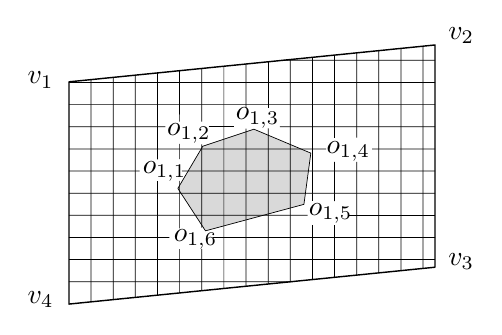
\begin{tikzpicture}[y=0.80pt, x=0.80pt, yscale=-\globalscale, xscale=\globalscale, inner sep=0pt, outer sep=0pt]
\path[draw=black,line join=round,line width=0.512pt] (18.6584,24.2061) -- (183.9870,7.5586) -- (183.9870,107.9380) -- (18.6584,124.5850) -- (18.6584,24.2061) -- cycle;



\path[draw=black,fill=cD9D9D9,line join=round,line width=0.256pt] (67.8359,72.3465) -- (79.1010,53.2824) -- (102.1880,45.5971) -- (127.8940,56.4066) -- (124.7750,79.5434) -- (80.3210,91.5016) -- (67.8359,72.3465) -- cycle;



\path[cm={{1.0,0.0,0.0,1.0,(0.0,27.0)}}] (0.0000,0.0000) node[above right] () {$v_1$};

\path[cm={{1.0,0.0,0.0,1.0,(0.0,126.0)}}] (0.0000,0.0000) node[above right] () {$v_4$};

\path[cm={{1.0,0.0,0.0,1.0,(190.0,7.0)}}] (0.0000,0.0000) node[above right] () {$v_2$};

\path[cm={{1.0,0.0,0.0,1.0,(190.0,109.0)}}] (0.0000,0.0000) node[above right] () {$v_3$};

\path[cm={{1.0,0.0,0.0,1.0,(52.0,69.0)}}] (0.0000,0.0000) node[above right] () {$o_{1,1}$};

\path[cm={{1.0,0.0,0.0,1.0,(63.0,52.0)}}] (0.0000,0.0000) node[above right] () {$o_{1,2}$};

\path[cm={{1.0,0.0,0.0,1.0,(94.0,45.0)}}] (0.0000,0.0000) node[above right] () {$o_{1,3}$};

\path[cm={{1.0,0.0,0.0,1.0,(135.0,60.0)}}] (0.0000,0.0000) node[above right] () {$o_{1,4}$};

\path[cm={{1.0,0.0,0.0,1.0,(127.0,88.0)}}] (0.0000,0.0000) node[above right] () {$o_{1,5}$};

\path[cm={{1.0,0.0,0.0,1.0,(66.0,100.0)}}] (0.0000,0.0000) node[above right] () {$o_{1,6}$};



\path[draw=black,line join=round,line width=0.256pt] (18.6285,54.5004) -- (134.7670,54.5001);



\path[draw=black,line join=round,line width=0.256pt] (155.5270,54.5004) -- (184.0610,54.5001);



\path[draw=black,line join=round,line width=0.256pt] (18.6285,24.5004) -- (184.0610,24.5001);



\path[draw=black,line join=round,line width=0.256pt] (18.6285,34.5004) -- (184.0610,34.5001);



\path[draw=black,line join=round,line width=0.256pt] (18.6285,44.5004) -- (62.1670,44.5003);



\path[draw=black,line join=round,line width=0.256pt] (81.7806,44.5003) -- (93.4071,44.5003);



\path[draw=black,line join=round,line width=0.256pt] (113.9670,44.5006) -- (184.0610,44.5001);



\path[draw=black,line join=round,line width=0.256pt] (18.6285,94.5004) -- (63.9474,94.5003);



\path[draw=black,line join=round,line width=0.256pt] (83.6273,94.5002) -- (184.0610,94.5001);



\path[draw=black,line join=round,line width=0.256pt] (18.6285,84.5004) -- (126.4200,84.5001);



\path[draw=black,line join=round,line width=0.256pt] (144.7140,84.5001) -- (184.0610,84.5001);



\path[draw=black,line join=round,line width=0.256pt] (18.6285,74.5004) -- (184.0610,74.5001);



\path[draw=black,line join=round,line width=0.256pt] (18.6285,64.5004) -- (50.5273,64.5003);



\path[draw=black,line join=round,line width=0.256pt] (69.6273,64.5003) -- (184.0610,64.5001);



\path[draw=black,line join=round,line width=0.256pt] (18.6285,104.5000) -- (184.0610,104.5000);



\path[draw=black,line join=round,line width=0.256pt] (18.6285,114.5000) -- (119.0600,114.5050);



\path[draw=black,line join=round,line width=0.256pt] (115.6280,14.5024) -- (184.0610,14.5001);



\path[draw=black,line join=round,line width=0.256pt] (118.6220,14.1766) -- (118.6250,114.6100);



\path[draw=black,line join=round,line width=0.256pt] (108.6230,15.1767) -- (108.6230,36.0018);



\path[draw=black,line join=round,line width=0.256pt] (108.6240,45.2420) -- (108.6260,115.6100);



\path[draw=black,line join=round,line width=0.256pt] (98.6223,16.1766) -- (98.6230,36.0302);



\path[draw=black,line join=round,line width=0.256pt] (98.6241,45.3706) -- (98.6257,116.6100);



\path[draw=black,line join=round,line width=0.256pt] (88.6223,17.1766) -- (88.6258,117.6100);



\path[draw=black,line join=round,line width=0.256pt] (78.6222,18.1766) -- (78.6228,42.2150);



\path[draw=black,line join=round,line width=0.256pt] (78.6234,52.4953) -- (78.6248,90.0419);



\path[draw=black,line join=round,line width=0.256pt] (78.6251,99.8153) -- (78.6258,118.6100);



\path[draw=black,line join=round,line width=0.256pt] (68.6223,19.1766) -- (68.6236,42.1817);



\path[draw=black,line join=round,line width=0.256pt] (68.6244,52.2773) -- (68.6245,59.1362);



\path[draw=black,line join=round,line width=0.256pt] (68.6249,68.8953) -- (68.6254,90.3623);



\path[draw=black,line join=round,line width=0.256pt] (68.6258,99.7889) -- (68.6263,119.6100);



\path[draw=black,line join=round,line width=0.256pt] (58.6232,20.1764) -- (58.6241,59.2753);



\path[draw=black,line join=round,line width=0.256pt] (58.6244,69.0756) -- (58.6263,120.6100);



\path[draw=black,line join=round,line width=0.256pt] (48.6232,21.1765) -- (48.6263,121.6100);



\path[draw=black,line join=round,line width=0.256pt] (28.6232,23.1764) -- (28.6263,123.6100);



\path[draw=black,line join=round,line width=0.256pt] (38.6232,22.1764) -- (38.6263,122.6100);



\path[draw=black,line join=round,line width=0.256pt] (128.6230,13.1767) -- (128.6240,78.0236);



\path[draw=black,line join=round,line width=0.256pt] (128.6250,88.7706) -- (128.6250,113.6100);



\path[draw=black,line join=round,line width=0.256pt] (138.6260,12.1767) -- (138.6260,49.4502);



\path[draw=black,line join=round,line width=0.256pt] (138.6270,60.3504) -- (138.6260,78.0353);



\path[draw=black,line join=round,line width=0.256pt] (138.6260,88.9086) -- (138.6250,112.6100);



\path[draw=black,line join=round,line width=0.256pt] (148.6270,11.1767) -- (148.6260,49.4287);



\path[draw=black,line join=round,line width=0.256pt] (148.6260,60.3688) -- (148.6250,111.5100);



\path[draw=black,line join=round,line width=0.256pt] (158.5930,10.1848) -- (158.5910,110.6180);



\path[draw=black,line join=round,line width=0.256pt] (168.6000,9.1981) -- (168.5980,109.6310);



\path[draw=black,line join=round,line width=0.256pt] (178.5500,8.1813) -- (178.5480,108.6140);




\end{tikzpicture}


  \caption[Grid decomposition]{A polygonal space where we want to find a coverage tour and visit all the points delimited by $v:=\{v_1,\dots,v_4\}$ except for the obstacle $o_1:=\{o_{1,1},\dots,o_{1,6}\}$. A way to cover the space is the grid decomposition that divides the polygon into equally sized cells and visits each cell except the obstacle.}
  \label{fig:gride}
\end{figure}
This methodology is termed grid decomposition\findex{grid decomposition} in~\fref{fig:gride}{Figure}. Another way is to sweep the polygon and divide it into sub-regions\findex{sub-regions} when the sweep line\findex{sweep line} encounters a change in connectivity. We implement this latter class in \fref{sec:cell-deco}{Section}.
Once the algorithm divides the free space into sub-region, it builds an adjacency graph\findex{adjacency graph}. The vertices contain the sub-regions and edges connect adjacent sub-regions~\citep{choset2005principles}. A covering order between the sub-region to derive the sequence of the coverage is then an exhaustive walkthrough of the adjacency graph with, e.g., depth-first search\findex{depth-first search} algorithm~\citep{choset2005principles}. Once divided the space and the order of the coverage, we need to cover each sub-region. We recall that a method is the boustrophedon motion that we discussed in \fref{cp:soa}{Chapter}. However, a generic nonholonomic mobile robot, such as the Opterra fixed-wing craft in the precision agriculture scenario in \fref{sec:motivation}{Section}, has limited maneuverability~\citep{mannadiar2010optimal,xu2011optimal,xu2014efficient}. For a generic aerial robot, it is preferred to have a large turning radius~\citep{wang2017curvature}; to this end, we propose a Zamboni-like motion. We introduced both the Zamboni- and boustrophedon-like motions in \fref{sec:path-wise}{Section}, whereas we implement them later in this chapter in \fref{sec:cov-motion}{Section}.

\subsection{Cellular decomposition of the space}
\label{sec:cell-deco}\findex{cellular decomposition}

In detail, a cellular decomposition decomposes the coverage space into non-overlapping sub-regions called cell\findex{cells}s. Let us define the robot's free space\findex{free space} or the coverage space\findex{coverage space} as $\mathcal{Q}^v$ for an inertial navigation frame $\mathcal{O}_W$. Physically, the free space is where the robot is free to move without intersecting an obstacle~\citep{choset2005principles}. Let $\mathcal{Q}^{o_i}\subset\mathbb{R}^2$ be the space delimited by the obstacle $o_i$. $\mathcal{Q}^v\subseteq\mathbb{R}^2$ contains all the points delimited by the vertices of the polygon $v$ except for $i$ obstacles delimited by the vertices of $i$ polygons $o_i$. The entire space in the polygon $v$, including all the obstacles $o_i$, is then $\mathcal{Q}:=(\bigcup_{i\in|o|}\mathcal{Q}^{o_i})\cup\mathcal{Q}^v$. 
\begin{figure}[h]
  \centering
  \fontfamily{phv}\selectfont
  
\definecolor{cD9D9D9}{RGB}{217,217,217}
\small

\def \globalscale {1.100000}
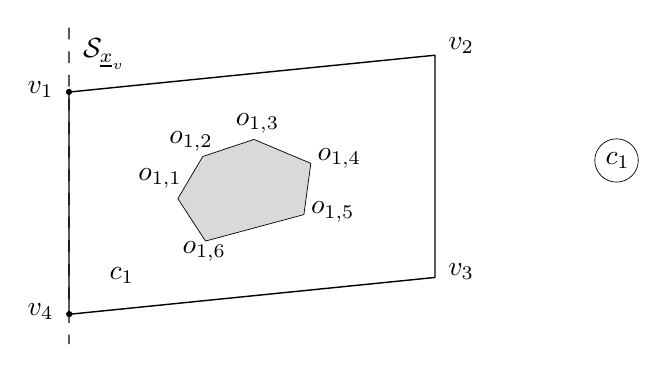
\begin{tikzpicture}[y=0.80pt, x=0.80pt, yscale=-\globalscale, xscale=\globalscale, inner sep=0pt, outer sep=0pt]
\path[draw=black,line join=round,line width=0.512pt] (18.6584,29.4064) -- (183.9870,12.7588) -- (183.9870,113.1380) -- (18.6584,129.7850) -- (18.6584,29.4064) -- cycle;

\path[draw=black,fill=black,line join=round,line width=0.512pt] (18.6440,28.2683) .. controls (19.2323,28.2683) and (19.7092,28.7453) .. (19.7092,29.3336) .. controls (19.7092,29.9219) and (19.2323,30.3988) .. (18.6440,30.3988) .. controls (18.0556,30.3988) and (17.5787,29.9219) .. (17.5787,29.3336) .. controls (17.5787,28.7453) and (18.0556,28.2683) .. (18.6440,28.2683) -- cycle;

\path[draw=black,fill=cD9D9D9,line join=round,line width=0.256pt] (67.8359,77.5468) -- (79.1010,58.4827) -- (102.1880,50.7974) -- (127.8940,61.6068) -- (124.7750,84.7435) -- (80.3210,96.7019) -- (67.8359,77.5468) -- cycle;

\path[draw=black,fill=black,line join=round,line width=0.512pt] (18.7577,128.6400) .. controls (19.3460,128.6400) and (19.8229,129.1170) .. (19.8229,129.7050) .. controls (19.8229,130.2930) and (19.3460,130.7700) .. (18.7577,130.7700) .. controls (18.1694,130.7700) and (17.6924,130.2930) .. (17.6924,129.7050) .. controls (17.6924,129.1170) and (18.1694,128.6400) .. (18.7577,128.6400) -- cycle;

\path[fill=black,line join=round,line width=0.256pt] (18.9784,10.9866) -- (18.9784,16.3199) -- (18.3384,16.3199) -- (18.3384,10.9866) -- (18.9784,10.9866) -- cycle(18.9784,21.6533) -- (18.9784,26.9866) -- (18.3384,26.9866) -- (18.3384,21.6533) -- (18.9784,21.6533) -- cycle(18.9784,32.3199) -- (18.9784,37.6533) -- (18.3384,37.6533) -- (18.3384,32.3199) -- (18.9784,32.3199) -- cycle(18.9784,42.9866) -- (18.9784,48.3199) -- (18.3384,48.3199) -- (18.3384,42.9866) -- (18.9784,42.9866) -- cycle(18.9784,53.6533) -- (18.9784,58.9866) -- (18.3384,58.9866) -- (18.3384,53.6533) -- (18.9784,53.6533) -- cycle(18.9784,64.3199) -- (18.9784,69.6533) -- (18.3384,69.6533) -- (18.3384,64.3199) -- (18.9784,64.3199) -- cycle(18.9784,74.9866) -- (18.9784,80.3199) -- (18.3384,80.3199) -- (18.3384,74.9866) -- (18.9784,74.9866) -- cycle(18.9784,85.6533) -- (18.9784,90.9866) -- (18.3384,90.9866) -- (18.3384,85.6533) -- (18.9784,85.6533) -- cycle(18.9784,96.3199) -- (18.9784,101.6530) -- (18.3384,101.6530) -- (18.3384,96.3199) -- (18.9784,96.3199) -- cycle(18.9784,106.9870) -- (18.9784,112.3200) -- (18.3384,112.3200) -- (18.3384,106.9870) -- (18.9784,106.9870) -- cycle(18.9784,117.6530) -- (18.9784,122.9870) -- (18.3384,122.9870) -- (18.3384,117.6530) -- (18.9784,117.6530) -- cycle(18.9784,128.3200) -- (18.9784,133.6530) -- (18.3384,133.6530) -- (18.3384,128.3200) -- (18.9784,128.3200) -- cycle(18.9784,138.9870) -- (18.9784,143.2150) -- (18.3384,143.2150) -- (18.3384,138.9870) -- (18.9784,138.9870) -- cycle(18.9784,0.3199) -- (18.9784,5.6533) -- (18.3384,5.6533) -- (18.3384,0.3199) -- (18.9784,0.3199) -- cycle;

\path[cm={{1.0,0.0,0.0,1.0,(0.0,32.0)}}] (0.0000,0.0000) node[above right] () {$v_1$};

\path[cm={{1.0,0.0,0.0,1.0,(0.0,132.0)}}] (0.0000,0.0000) node[above right] () {$v_4$};

\path[cm={{1.0,0.0,0.0,1.0,(190.0,12.0)}}] (0.0000,0.0000) node[above right] () {$v_2$};

\path[cm={{1.0,0.0,0.0,1.0,(190.0,114.0)}}] (0.0000,0.0000) node[above right] () {$v_3$};

\path[cm={{1.0,0.0,0.0,1.0,(50.0,73.0)}}] (0.0000,0.0000) node[above right] () {$o_{1,1}$};

\path[cm={{1.0,0.0,0.0,1.0,(64.0,56.0)}}] (0.0000,0.0000) node[above right] () {$o_{1,2}$};

\path[cm={{1.0,0.0,0.0,1.0,(94.0,48.0)}}] (0.0000,0.0000) node[above right] () {$o_{1,3}$};

\path[cm={{1.0,0.0,0.0,1.0,(131.0,64.0)}}] (0.0000,0.0000) node[above right] () {$o_{1,4}$};

\path[cm={{1.0,0.0,0.0,1.0,(128.0,88.0)}}] (0.0000,0.0000) node[above right] () {$o_{1,5}$};

\path[cm={{1.0,0.0,0.0,1.0,(70.0,106.0)}}] (0.0000,0.0000) node[above right] () {$o_{1,6}$};

\path[cm={{1.0,0.0,0.0,1.0,(25.0,19.0)}}] (0.0000,0.0000) node[above right] () {$\mathcal{S}_{\underline{x}_v}$};

\path[draw=black,line join=round,line width=0.256pt] (265.9760,60.3019) ellipse (0.2763cm and 0.2749cm);

\path[cm={{1.0,0.0,0.0,1.0,(261.0,64.0)}}] (0.0000,0.0000) node[above right] () {$c_1$};


\path[cm={{1.0,0.0,0.0,1.0,(37.0,116.0)}}] (0.0000,0.0000) node[above right] () {$c_1$};

\end{tikzpicture}

  \caption[Initial step of the boustrophedon decomposition]{The boustrophedon decomposition for coverage path planning sweeps the space and adds cells in case the sweeping line encounters a change in connectivity. Figure shows an initial step with $c_1$ the first cell formed.}
  \label{fig:bcd2}
\end{figure}
In \fref{fig:bcd2}{Figure}, the polygon is delimited by $v:=\{v_1,\dots,v_4\}$ and forms $\mathcal{Q}^v$, whereas the obstacle by $o_1:=\{o_{1,1},\dots,o_{1,6}\}$ and forms $\mathcal{Q}^{o_1}$. The union of these two is then $\mathcal{Q}$.

An important approach in the polygonal environment is the boustrophedon decomposition\findex{boustrophedon decomposition}~\citep{choset2000coverage}. For non-polygonal environments where $v$ and $o_i$ are, e.g., elliptical functions, a significant result is the decomposition in terms of critical points of Morse functions\findex{Morse functions}~\citep{choset2000exact}. Both the boustrophedon decomposition and decomposition in terms of critical points of Morse functions sweep $\mathcal{Q}$ with a line and decompose $\mathcal{Q}^v$ adding a cell in case of a change in connectivity or when they encounter a critical point~\citep{choset2000coverage,choset2001coverage,choset2005principles}. 
\begin{figure}[h]
  \centering
  \fontfamily{phv}\selectfont
  
\definecolor{cD9D9D9}{RGB}{217,217,217}
\small
\def \globalscale {1.000000}
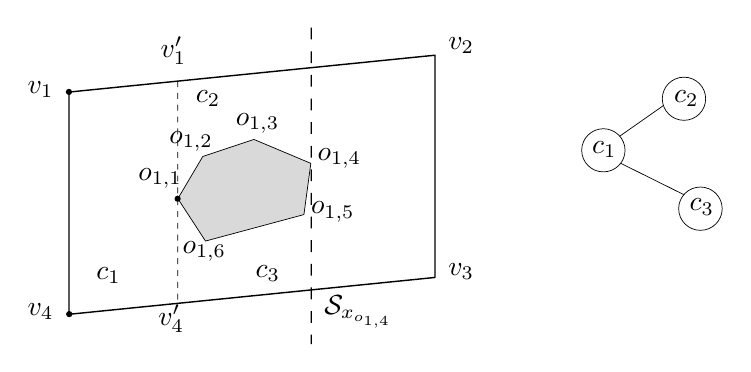
\begin{tikzpicture}[y=0.80pt, x=0.80pt, yscale=-\globalscale, xscale=\globalscale, inner sep=0pt, outer sep=0pt]
\path[draw=black,line join=round,line width=0.512pt] (18.6584,29.4063) -- (183.9870,12.7587) -- (183.9870,113.1380) -- (18.6584,129.7850) -- (18.6584,29.4063) -- cycle;

\path[draw=black,fill=black,line join=round,line width=0.512pt] (18.6440,28.2683) .. controls (19.2323,28.2683) and (19.7092,28.7452) .. (19.7092,29.3336) .. controls (19.7092,29.9218) and (19.2323,30.3988) .. (18.6440,30.3988) .. controls (18.0557,30.3988) and (17.5787,29.9218) .. (17.5787,29.3336) .. controls (17.5787,28.7452) and (18.0557,28.2683) .. (18.6440,28.2683) -- cycle;

\path[draw=black,fill=cD9D9D9,line join=round,line width=0.256pt] (67.8359,77.5466) -- (79.1010,58.4826) -- (102.1880,50.7973) -- (127.8940,61.6068) -- (124.7750,84.7435) -- (80.3210,96.7018) -- (67.8359,77.5466) -- cycle;

\path[draw=black,fill=black,line join=round,line width=0.512pt] (18.7577,128.6400) .. controls (19.3460,128.6400) and (19.8230,129.1170) .. (19.8230,129.7050) .. controls (19.8230,130.2930) and (19.3460,130.7700) .. (18.7577,130.7700) .. controls (18.1694,130.7700) and (17.6925,130.2930) .. (17.6925,129.7050) .. controls (17.6925,129.1170) and (18.1694,128.6400) .. (18.7577,128.6400) -- cycle;

\path[cm={{1.0,0.0,0.0,1.0,(0.0,32.0)}}] (0.0000,0.0000) node[above right] () {$v_1$};

\path[cm={{1.0,0.0,0.0,1.0,(0.0,132.0)}}] (0.0000,0.0000) node[above right] () {$v_4$};

\path[cm={{1.0,0.0,0.0,1.0,(190.0,12.0)}}] (0.0000,0.0000) node[above right] () {$v_2$};

\path[cm={{1.0,0.0,0.0,1.0,(190.0,114.0)}}] (0.0000,0.0000) node[above right] () {$v_3$};

\path[cm={{1.0,0.0,0.0,1.0,(50.0,73.0)}}] (0.0000,0.0000) node[above right] () {$o_{1,1}$};

\path[cm={{1.0,0.0,0.0,1.0,(64.0,56.0)}}] (0.0000,0.0000) node[above right] () {$o_{1,2}$};

\path[cm={{1.0,0.0,0.0,1.0,(94.0,48.0)}}] (0.0000,0.0000) node[above right] () {$o_{1,3}$};

\path[cm={{1.0,0.0,0.0,1.0,(131.0,64.0)}}] (0.0000,0.0000) node[above right] () {$o_{1,4}$};

\path[cm={{1.0,0.0,0.0,1.0,(128.0,88.0)}}] (0.0000,0.0000) node[above right] () {$o_{1,5}$};

\path[cm={{1.0,0.0,0.0,1.0,(70.0,106.0)}}] (0.0000,0.0000) node[above right] () {$o_{1,6}$};

\path[fill=black,line join=round,line width=0.256pt] (128.3960,10.9866) -- (128.3960,16.3199) -- (127.7560,16.3199) -- (127.7560,10.9866) -- (128.3960,10.9866) -- cycle(128.3960,21.6533) -- (128.3960,26.9866) -- (127.7560,26.9866) -- (127.7560,21.6533) -- (128.3960,21.6533) -- cycle(128.3960,32.3199) -- (128.3960,37.6533) -- (127.7560,37.6533) -- (127.7560,32.3199) -- (128.3960,32.3199) -- cycle(128.3960,42.9866) -- (128.3960,48.3199) -- (127.7560,48.3199) -- (127.7560,42.9866) -- (128.3960,42.9866) -- cycle(128.3960,53.6533) -- (128.3960,58.9866) -- (127.7560,58.9866) -- (127.7560,53.6533) -- (128.3960,53.6533) -- cycle(128.3960,64.3199) -- (128.3960,69.6533) -- (127.7560,69.6533) -- (127.7560,64.3199) -- (128.3960,64.3199) -- cycle(128.3960,74.9866) -- (128.3960,80.3199) -- (127.7560,80.3199) -- (127.7560,74.9866) -- (128.3960,74.9866) -- cycle(128.3960,85.6533) -- (128.3960,90.9866) -- (127.7560,90.9866) -- (127.7560,85.6533) -- (128.3960,85.6533) -- cycle(128.3960,96.3199) -- (128.3960,101.6530) -- (127.7560,101.6530) -- (127.7560,96.3199) -- (128.3960,96.3199) -- cycle(128.3960,106.9870) -- (128.3960,112.3200) -- (127.7560,112.3200) -- (127.7560,106.9870) -- (128.3960,106.9870) -- cycle(128.3960,117.6530) -- (128.3960,122.9870) -- (127.7560,122.9870) -- (127.7560,117.6530) -- (128.3960,117.6530) -- cycle(128.3960,128.3200) -- (128.3960,133.6530) -- (127.7560,133.6530) -- (127.7560,128.3200) -- (128.3960,128.3200) -- cycle(128.3960,138.9870) -- (128.3960,143.2150) -- (127.7560,143.2150) -- (127.7560,138.9870) -- (128.3960,138.9870) -- cycle(128.3960,0.3199) -- (128.3960,5.6533) -- (127.7560,5.6533) -- (127.7560,0.3199) -- (128.3960,0.3199) -- cycle;

\path[fill=black,line join=round,line width=0.256pt] (67.9513,29.7995) -- (67.9513,32.4662) -- (67.6313,32.4662) -- (67.6313,29.7995) -- (67.9513,29.7995) -- cycle(67.9513,35.1329) -- (67.9513,37.7995) -- (67.6313,37.7995) -- (67.6313,35.1329) -- (67.9513,35.1329) -- cycle(67.9513,40.4662) -- (67.9513,43.1329) -- (67.6313,43.1329) -- (67.6313,40.4662) -- (67.9513,40.4662) -- cycle(67.9513,45.7995) -- (67.9513,48.4662) -- (67.6313,48.4662) -- (67.6313,45.7995) -- (67.9513,45.7995) -- cycle(67.9513,51.1329) -- (67.9513,53.7995) -- (67.6313,53.7995) -- (67.6313,51.1329) -- (67.9513,51.1329) -- cycle(67.9513,56.4662) -- (67.9513,59.1329) -- (67.6313,59.1329) -- (67.6313,56.4662) -- (67.9513,56.4662) -- cycle(67.9513,61.7995) -- (67.9513,64.4662) -- (67.6313,64.4662) -- (67.6313,61.7995) -- (67.9513,61.7995) -- cycle(67.9513,67.1329) -- (67.9513,69.7995) -- (67.6313,69.7995) -- (67.6313,67.1329) -- (67.9513,67.1329) -- cycle(67.9513,72.4662) -- (67.9513,75.1329) -- (67.6313,75.1329) -- (67.6313,72.4662) -- (67.9513,72.4662) -- cycle(67.9513,77.7995) -- (67.9513,80.4662) -- (67.6313,80.4662) -- (67.6313,77.7995) -- (67.9513,77.7995) -- cycle(67.9513,83.1329) -- (67.9513,85.7995) -- (67.6313,85.7995) -- (67.6313,83.1329) -- (67.9513,83.1329) -- cycle(67.9513,88.4662) -- (67.9513,91.1329) -- (67.6313,91.1329) -- (67.6313,88.4662) -- (67.9513,88.4662) -- cycle(67.9513,93.7995) -- (67.9513,96.4662) -- (67.6313,96.4662) -- (67.6313,93.7995) -- (67.9513,93.7995) -- cycle(67.9513,99.1329) -- (67.9513,101.8000) -- (67.6313,101.8000) -- (67.6313,99.1329) -- (67.9513,99.1329) -- cycle(67.9513,104.4660) -- (67.9513,107.1330) -- (67.6313,107.1330) -- (67.6313,104.4660) -- (67.9513,104.4660) -- cycle(67.9513,109.8000) -- (67.9513,112.4660) -- (67.6313,112.4660) -- (67.6313,109.8000) -- (67.9513,109.8000) -- cycle(67.9513,115.1330) -- (67.9513,117.8000) -- (67.6313,117.8000) -- (67.6313,115.1330) -- (67.9513,115.1330) -- cycle(67.9513,120.4660) -- (67.9513,123.1330) -- (67.6313,123.1330) -- (67.6313,120.4660) -- (67.9513,120.4660) -- cycle(67.9513,24.4662) -- (67.9513,27.1329) -- (67.6313,27.1329) -- (67.6313,24.4662) -- (67.9513,24.4662) -- cycle;



\path[draw=black,fill=black,line join=round,line width=0.512pt] (67.7196,76.5121) .. controls (68.3079,76.5121) and (68.7848,76.9890) .. (68.7848,77.5774) .. controls (68.7848,78.1656) and (68.3079,78.6426) .. (67.7196,78.6426) .. controls (67.1313,78.6426) and (66.6544,78.1656) .. (66.6544,77.5774) .. controls (66.6544,76.9890) and (67.1313,76.5121) .. (67.7196,76.5121) -- cycle;



\path[cm={{1.0,0.0,0.0,1.0,(134.0,136.0)}}] (0.0000,0.0000) node[above right] () {$\mathcal{S}_{x_{o_{1,4}}}$};



\path[cm={{1.0,0.0,0.0,1.0,(60.0,17.0)}}] (0.0000,0.0000) node[above right] () {$v_1'$};



\path[cm={{1.0,0.0,0.0,1.0,(59.0,138.0)}}] (0.0000,0.0000) node[above right] () {$v_4'$};



\path[draw=black,line join=round,line width=0.256pt] (260.0330,45.9693) .. controls (265.4410,45.9693) and (269.8250,50.3308) .. (269.8250,55.7110) .. controls (269.8250,61.0912) and (265.4410,65.4527) .. (260.0330,65.4527) .. controls (254.6250,65.4527) and (250.2410,61.0912) .. (250.2410,55.7110) .. controls (250.2410,50.3308) and (254.6250,45.9693) .. (260.0330,45.9693) -- cycle;



\path[cm={{1.0,0.0,0.0,1.0,(255.0,59.0)}}] (0.0000,0.0000) node[above right] () {$c_1$};



\path[draw=black,line join=round,line width=0.256pt] (303.8700,82.0760) ellipse (0.2763cm and 0.2749cm);



\path[cm={{1.0,0.0,0.0,1.0,(299.0,85.0)}}] (0.0000,0.0000) node[above right] () {$c_3$};



\path[draw=black,line join=round,line width=0.256pt] (296.4430,22.6787) .. controls (301.8500,22.6787) and (306.2340,27.0402) .. (306.2340,32.4204) .. controls (306.2340,37.8006) and (301.8500,42.1621) .. (296.4430,42.1621) .. controls (291.0350,42.1621) and (286.6510,37.8006) .. (286.6510,32.4204) .. controls (286.6510,27.0402) and (291.0350,22.6787) .. (296.4430,22.6787) -- cycle;

\path[cm={{1.0,0.0,0.0,1.0,(292.0,36.0)}}] (0.0000,0.0000) node[above right] () {$c_2$};

\path[draw=black,line join=round,line width=0.256pt] (267.9900,61.6406) -- (296.5230,75.8005);

\path[draw=black,line join=round,line width=0.256pt] (267.5100,49.2690) -- (287.1900,35.4824);

\path[cm={{1.0,0.0,0.0,1.0,(31.0,116.0)}}] (0.0000,0.0000) node[above right] () {$c_1$};

\path[cm={{1.0,0.0,0.0,1.0,(76.0,36.0)}}] (0.0000,0.0000) node[above right] () {$c_2$};

\path[cm={{1.0,0.0,0.0,1.0,(103.0,115.0)}}] (0.0000,0.0000) node[above right] () {$c_3$};

\end{tikzpicture}


  \caption[Intermediate step of the boustrophedon decomposition]{An intermediate step of the boustrophedon decomposition, with $c_2,c_3$ formed at the first encounter of the obstacle $o_1$. The black points indicate the critical points or changes in connectivity.
  }
  \label{fig:bcd3}
\end{figure}
In \fref{fig:bcd3}{Figure}, the change in connectivity happens when the sweeping line encounters the obstacle $o_1$. This approach optimizes the neighboring cells that can be thus aggregated as opposed to, e.g., trapezoidal decomposition\findex{trapezoidal decomposition}~\citep{galceran2013survey} in \fref{fig:trap}{Figure}, which splits the space into cells when it encounters a vertex~\citep{lavalle2006planning}.
\begin{figure}[h]
  \centering
  \fontfamily{phv}\selectfont
  
\definecolor{cD9D9D9}{RGB}{217,217,217}
\small

\def \globalscale {1.100000}
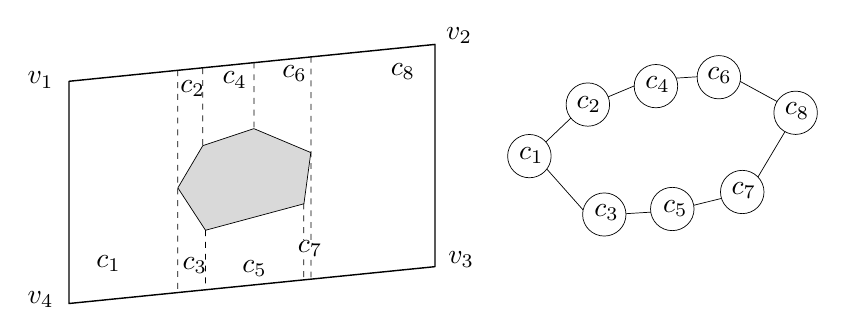
\begin{tikzpicture}[y=0.80pt, x=0.80pt, yscale=-\globalscale, xscale=\globalscale, inner sep=0pt, outer sep=0pt]
\path[draw=black,line join=round,line width=0.512pt] (18.6583,24.9551) -- (183.9870,8.3075) -- (183.9870,108.6870) -- (18.6583,125.3340) -- (18.6583,24.9551) -- cycle;




\path[draw=black,fill=cD9D9D9,line join=round,line width=0.256pt] (67.8359,73.0953) -- (79.1010,54.0313) -- (102.1880,46.3460) -- (127.8940,57.1555) -- (124.7750,80.2922) -- (80.3210,92.2505) -- (67.8359,73.0953) -- cycle;



\path[cm={{1.0,0.0,0.0,1.0,(0.0,28.0)}}] (0.0000,0.0000) node[above right] () {$v_1$};



\path[cm={{1.0,0.0,0.0,1.0,(0.0,127.0)}}] (0.0000,0.0000) node[above right] () {$v_4$};



\path[cm={{1.0,0.0,0.0,1.0,(189.0,8.0)}}] (0.0000,0.0000) node[above right] () {$v_2$};



\path[cm={{1.0,0.0,0.0,1.0,(190.0,109.0)}}] (0.0000,0.0000) node[above right] () {$v_3$};



\path[fill=black,line join=round,line width=0.256pt] (67.9514,25.3483) -- (67.9514,28.0150) -- (67.6314,28.0150) -- (67.6314,25.3483) -- (67.9514,25.3483) -- cycle(67.9514,30.6816) -- (67.9514,33.3483) -- (67.6314,33.3483) -- (67.6314,30.6816) -- (67.9514,30.6816) -- cycle(67.9514,36.0150) -- (67.9514,38.6816) -- (67.6314,38.6816) -- (67.6314,36.0150) -- (67.9514,36.0150) -- cycle(67.9514,41.3483) -- (67.9514,44.0150) -- (67.6314,44.0150) -- (67.6314,41.3483) -- (67.9514,41.3483) -- cycle(67.9514,46.6816) -- (67.9514,49.3483) -- (67.6314,49.3483) -- (67.6314,46.6816) -- (67.9514,46.6816) -- cycle(67.9514,52.0150) -- (67.9514,54.6816) -- (67.6314,54.6816) -- (67.6314,52.0150) -- (67.9514,52.0150) -- cycle(67.9514,57.3483) -- (67.9514,60.0150) -- (67.6314,60.0150) -- (67.6314,57.3483) -- (67.9514,57.3483) -- cycle(67.9514,62.6816) -- (67.9514,65.3483) -- (67.6314,65.3483) -- (67.6314,62.6816) -- (67.9514,62.6816) -- cycle(67.9514,68.0150) -- (67.9514,70.6816) -- (67.6314,70.6816) -- (67.6314,68.0150) -- (67.9514,68.0150) -- cycle(67.9514,73.3483) -- (67.9514,76.0150) -- (67.6314,76.0150) -- (67.6314,73.3483) -- (67.9514,73.3483) -- cycle(67.9514,78.6816) -- (67.9514,81.3483) -- (67.6314,81.3483) -- (67.6314,78.6816) -- (67.9514,78.6816) -- cycle(67.9514,84.0150) -- (67.9514,86.6816) -- (67.6314,86.6816) -- (67.6314,84.0150) -- (67.9514,84.0150) -- cycle(67.9514,89.3483) -- (67.9514,92.0150) -- (67.6314,92.0150) -- (67.6314,89.3483) -- (67.9514,89.3483) -- cycle(67.9514,94.6816) -- (67.9514,97.3483) -- (67.6314,97.3483) -- (67.6314,94.6816) -- (67.9514,94.6816) -- cycle(67.9514,100.0150) -- (67.9514,102.6820) -- (67.6314,102.6820) -- (67.6314,100.0150) -- (67.9514,100.0150) -- cycle(67.9514,105.3480) -- (67.9514,108.0150) -- (67.6314,108.0150) -- (67.6314,105.3480) -- (67.9514,105.3480) -- cycle(67.9514,110.6820) -- (67.9514,113.3480) -- (67.6314,113.3480) -- (67.6314,110.6820) -- (67.9514,110.6820) -- cycle(67.9514,116.0150) -- (67.9514,118.6820) -- (67.6314,118.6820) -- (67.6314,116.0150) -- (67.9514,116.0150) -- cycle(67.9514,20.0150) -- (67.9514,22.6816) -- (67.6314,22.6816) -- (67.6314,20.0150) -- (67.9514,20.0150) -- cycle;

\path[fill=black,line join=round,line width=0.256pt] (128.1570,19.2150) -- (128.1570,21.8817) -- (127.8370,21.8817) -- (127.8370,19.2150) -- (128.1570,19.2150) -- cycle(128.1570,24.5484) -- (128.1570,27.2150) -- (127.8370,27.2150) -- (127.8370,24.5484) -- (128.1570,24.5484) -- cycle(128.1570,29.8817) -- (128.1570,32.5484) -- (127.8370,32.5484) -- (127.8370,29.8817) -- (128.1570,29.8817) -- cycle(128.1570,35.2150) -- (128.1570,37.8817) -- (127.8370,37.8817) -- (127.8370,35.2150) -- (128.1570,35.2150) -- cycle(128.1570,40.5484) -- (128.1570,43.2150) -- (127.8370,43.2150) -- (127.8370,40.5484) -- (128.1570,40.5484) -- cycle(128.1570,45.8817) -- (128.1570,48.5484) -- (127.8370,48.5484) -- (127.8370,45.8817) -- (128.1570,45.8817) -- cycle(128.1570,51.2150) -- (128.1570,53.8817) -- (127.8370,53.8817) -- (127.8370,51.2150) -- (128.1570,51.2150) -- cycle(128.1570,56.5484) -- (128.1570,59.2150) -- (127.8370,59.2150) -- (127.8370,56.5484) -- (128.1570,56.5484) -- cycle(128.1570,61.8817) -- (128.1570,64.5484) -- (127.8370,64.5484) -- (127.8370,61.8817) -- (128.1570,61.8817) -- cycle(128.1570,67.2150) -- (128.1570,69.8817) -- (127.8370,69.8817) -- (127.8370,67.2150) -- (128.1570,67.2150) -- cycle(128.1570,72.5484) -- (128.1570,75.2150) -- (127.8370,75.2150) -- (127.8370,72.5484) -- (128.1570,72.5484) -- cycle(128.1570,77.8817) -- (128.1570,80.5484) -- (127.8370,80.5484) -- (127.8370,77.8817) -- (128.1570,77.8817) -- cycle(128.1570,83.2150) -- (128.1570,85.8817) -- (127.8370,85.8817) -- (127.8370,83.2150) -- (128.1570,83.2150) -- cycle(128.1570,88.5484) -- (128.1570,91.2150) -- (127.8370,91.2150) -- (127.8370,88.5484) -- (128.1570,88.5484) -- cycle(128.1570,93.8817) -- (128.1570,96.5484) -- (127.8370,96.5484) -- (127.8370,93.8817) -- (128.1570,93.8817) -- cycle(128.1570,13.8817) -- (128.1570,16.5484) -- (127.8370,16.5484) -- (127.8370,13.8817) -- (128.1570,13.8817) -- cycle;



\path[fill=black,line join=round,line width=0.256pt] (128.1570,110.9160) -- (128.1570,113.5830) -- (127.8370,113.5830) -- (127.8370,110.9160) -- (128.1570,110.9160) -- cycle(128.1570,105.5830) -- (128.1570,108.2490) -- (127.8370,108.2490) -- (127.8370,105.5830) -- (128.1570,105.5830) -- cycle;



\path[draw=black,line join=round,line width=0.256pt] (283.7740,27.1487) ellipse (0.2763cm and 0.2749cm);



\path[cm={{1.0,0.0,0.0,1.0,(279.0,30.0)}}] (0.0000,0.0000) node[above right] () {$c_4$};



\path[cm={{1.0,0.0,0.0,1.0,(31.0,111.0)}}] (0.0000,0.0000) node[above right] () {$c_1$};



\path[cm={{1.0,0.0,0.0,1.0,(69.0,32.0)}}] (0.0000,0.0000) node[above right] () {$c_2$};



\path[cm={{1.0,0.0,0.0,1.0,(164.0,24.0)}}] (0.0000,0.0000) node[above right] () {$c_8$};



\path[cm={{1.0,0.0,0.0,1.0,(70.0,112.0)}}] (0.0000,0.0000) node[above right] () {$c_3$};



\path[draw=black,line join=round,line width=0.256pt] (226.6150,58.7603) ellipse (0.2763cm and 0.2749cm);



\path[cm={{1.0,0.0,0.0,1.0,(222.0,62.0)}}] (0.0000,0.0000) node[above right] () {$c_1$};



\path[draw=black,line join=round,line width=0.256pt] (260.4520,75.3837) .. controls (265.8590,75.3837) and (270.2430,79.7451) .. (270.2430,85.1254) .. controls (270.2430,90.5056) and (265.8590,94.8671) .. (260.4520,94.8671) .. controls (255.0440,94.8671) and (250.6600,90.5056) .. (250.6600,85.1254) .. controls (250.6600,79.7451) and (255.0440,75.3837) .. (260.4520,75.3837) -- cycle;



\path[cm={{1.0,0.0,0.0,1.0,(256.0,88.0)}}] (0.0000,0.0000) node[above right] () {$c_3$};



\path[draw=black,line join=round,line width=0.256pt] (253.0240,35.4697) ellipse (0.2763cm and 0.2749cm);



\path[cm={{1.0,0.0,0.0,1.0,(248.0,39.0)}}] (0.0000,0.0000) node[above right] () {$c_2$};



\path[draw=black,line join=round,line width=0.256pt] (234.5710,64.6898) -- (250.8100,82.9987);



\path[draw=black,line join=round,line width=0.256pt] (234.0910,52.3182) -- (245.4260,41.5057);



\path[draw=black,line join=round,line width=0.256pt] (262.1050,32.0142) -- (274.0520,27.0187);



\path[fill=black,line join=round,line width=0.256pt] (79.2593,24.3795) -- (79.2593,27.0461) -- (78.9393,27.0461) -- (78.9393,24.3795) -- (79.2593,24.3795) -- cycle(79.2594,29.7128) -- (79.2594,32.3795) -- (78.9394,32.3795) -- (78.9393,29.7128) -- (79.2594,29.7128) -- cycle(79.2594,35.0461) -- (79.2594,37.7128) -- (78.9394,37.7128) -- (78.9394,35.0461) -- (79.2594,35.0461) -- cycle(79.2594,40.3795) -- (79.2595,43.0461) -- (78.9395,43.0461) -- (78.9394,40.3795) -- (79.2594,40.3795) -- cycle(79.2595,45.7128) -- (79.2595,48.3795) -- (78.9395,48.3795) -- (78.9395,45.7128) -- (79.2595,45.7128) -- cycle(79.2595,51.0461) -- (79.2596,53.7128) -- (78.9395,53.7128) -- (78.9395,51.0461) -- (79.2595,51.0461) -- cycle(79.2593,19.0461) -- (79.2593,21.7128) -- (78.9393,21.7128) -- (78.9393,19.0461) -- (79.2593,19.0461) -- cycle;



\path[fill=black,line join=round,line width=0.256pt] (102.3660,21.8091) -- (102.3660,24.4758) -- (102.0460,24.4758) -- (102.0460,21.8091) -- (102.3660,21.8091) -- cycle(102.3660,27.1425) -- (102.3660,29.8091) -- (102.0460,29.8091) -- (102.0460,27.1425) -- (102.3660,27.1425) -- cycle(102.3660,32.4758) -- (102.3660,35.1425) -- (102.0460,35.1425) -- (102.0460,32.4758) -- (102.3660,32.4758) -- cycle(102.3660,37.8091) -- (102.3660,40.4758) -- (102.0460,40.4758) -- (102.0460,37.8091) -- (102.3660,37.8091) -- cycle(102.3660,43.1425) -- (102.3660,45.8091) -- (102.0460,45.8091) -- (102.0460,43.1425) -- (102.3660,43.1425) -- cycle(102.3660,16.4758) -- (102.3660,19.1425) -- (102.0460,19.1425) -- (102.0460,16.4758) -- (102.3660,16.4758) -- cycle;



\path[fill=black,line join=round,line width=0.256pt] (80.5200,97.5339) -- (80.5201,100.2010) -- (80.2001,100.2010) -- (80.2000,97.5339) -- (80.5200,97.5339) -- cycle(80.5201,102.8670) -- (80.5201,105.5340) -- (80.2001,105.5340) -- (80.2001,102.8670) -- (80.5201,102.8670) -- cycle(80.5202,108.2010) -- (80.5202,110.8670) -- (80.2002,110.8670) -- (80.2002,108.2010) -- (80.5202,108.2010) -- cycle(80.5202,113.5340) -- (80.5203,116.2010) -- (80.2003,116.2010) -- (80.2002,113.5340) -- (80.5202,113.5340) -- cycle(80.5203,118.8670) -- (80.5203,119.2830) -- (80.2003,119.2830) -- (80.2003,118.8670) -- (80.5203,118.8670) -- cycle(80.5199,92.2006) -- (80.5200,94.8672) -- (80.2000,94.8672) -- (80.1999,92.2006) -- (80.5199,92.2006) -- cycle;



\path[fill=black,line join=round,line width=0.256pt] (124.8630,85.5283) -- (124.8630,88.1949) -- (124.5430,88.1949) -- (124.5430,85.5283) -- (124.8630,85.5283) -- cycle(124.8630,90.8616) -- (124.8630,93.5283) -- (124.5430,93.5283) -- (124.5430,90.8616) -- (124.8630,90.8616) -- cycle(124.8630,96.1949) -- (124.8630,96.7428) -- (124.5430,96.7428) -- (124.5430,96.1949) -- (124.8630,96.1949) -- cycle(124.8630,80.1949) -- (124.8630,82.8616) -- (124.5430,82.8616) -- (124.5430,80.1949) -- (124.8630,80.1949) -- cycle;



\path[fill=black,line join=round,line width=0.256pt] (124.8630,110.7160) -- (124.8630,113.3830) -- (124.5430,113.3830) -- (124.5430,110.7160) -- (124.8630,110.7160) -- cycle(124.8630,105.3830) -- (124.8630,108.0490) -- (124.5430,108.0490) -- (124.5430,105.3830) -- (124.8630,105.3830) -- cycle;



\path[cm={{1.0,0.0,0.0,1.0,(88.0,28.0)}}] (0.0000,0.0000) node[above right] () {$c_4$};



\path[cm={{1.0,0.0,0.0,1.0,(115.0,25.0)}}] (0.0000,0.0000) node[above right] () {$c_6$};



\path[cm={{1.0,0.0,0.0,1.0,(97.0,113.0)}}] (0.0000,0.0000) node[above right] () {$c_5$};



\path[cm={{1.0,0.0,0.0,1.0,(122.0,104.0)}}] (0.0000,0.0000) node[above right] () {$c_7$};



\path[draw=black,line join=round,line width=0.256pt] (291.1610,82.6401) ellipse (0.2763cm and 0.2749cm);



\path[cm={{1.0,0.0,0.0,1.0,(287.0,86.0)}}] (0.0000,0.0000) node[above right] () {$c_5$};



\path[draw=black,line join=round,line width=0.256pt] (312.2010,23.1201) ellipse (0.2763cm and 0.2749cm);



\path[cm={{1.0,0.0,0.0,1.0,(307.0,26.0)}}] (0.0000,0.0000) node[above right] () {$c_6$};



\path[draw=black,line join=round,line width=0.256pt] (322.7610,74.9601) ellipse (0.2763cm and 0.2749cm);



\path[cm={{1.0,0.0,0.0,1.0,(318.0,78.0)}}] (0.0000,0.0000) node[above right] () {$c_7$};



\path[draw=black,line join=round,line width=0.256pt] (346.8680,39.1857) ellipse (0.2763cm and 0.2749cm);



\path[cm={{1.0,0.0,0.0,1.0,(342.0,42.0)}}] (0.0000,0.0000) node[above right] () {$c_8$};



\path[draw=black,line join=round,line width=0.256pt] (270.2760,84.7587) -- (281.4500,84.0653);



\path[draw=black,line join=round,line width=0.256pt] (300.8880,80.9471) -- (313.4220,77.8538);



\path[draw=black,line join=round,line width=0.256pt] (329.8480,68.2004) -- (342.1150,47.6137);



\path[draw=black,line join=round,line width=0.256pt] (321.7150,24.9500) -- (338.4350,34.0699);



\path[draw=black,line join=round,line width=0.256pt] (302.5050,22.9167) -- (292.8850,23.5300);




\end{tikzpicture}


  \caption[Trapezoidal decomposition]{In the trapezoidal decomposition a lot of small cells are created (i.e., the cells $c_2,c_3,c_7$) that can be otherwise merged resulting in disconnected coverage. Boustrophedon decomposition solves the problem by splitting/merging the cells at critical points rather than at vertices. The resulting tour has eight cells as opposed to four cells with boustrophedon decomposition in \fref{fig:bcd4}{Figure}.}
  \label{fig:trap}
\end{figure}
For the decomposition in terms of critical points of Morse functions, the intuition of using critical points\findex{critical points}~\citep{choset2000exact} comes from some early studies on roadmaps\findex{roadmaps}~\citep{canny1988complexity,canny1988constructing,canny1993opportunistic}. Notably, these studies show that topology\findex{topology} (i.e., connectivity) changes only at critical points of a sweeping function restricted to the boundaries of obstacles. We briefly summarize some findings~\citep{choset2000exact} for this latter method before discussing the coverage motion for the cells.

Let us define $\mathcal{S}_\lambda$ as the vertical sweeping function that sweeps $\mathcal{Q}$. A change in the value of $\lambda$ moves the function in $\mathcal{Q}$. Let further $\overline{x}_v,\underline{x}_v$ be the highest and lowest coordinate $x$ of all the vertices in $v$, i.e., $\lambda\in[\underline{x}_v,\overline{x}_v]$. If we refer to the sweeping function with at a specific point in space as a slice, we can express the entire space as the union of all the slices, i.e., $\mathcal{Q}=\cup_{\lambda}\mathcal{S}_\lambda$. Let us further define the slice contained in the free space $\mathcal{S}^v_\lambda:=\mathcal{S}_\lambda\cap\mathcal{Q}^{v}$.
At this point, a change in connectivity of $\mathcal{S}^v$ means that the original cell has to be closed and two more opened, or that two cells are closed and one is opened respectively when the connectivity increases or decreases~\citep{choset2000exact}. 
\begin{figure}[h]
  \centering
  \fontfamily{phv}\selectfont
  
\definecolor{cD9D9D9}{RGB}{217,217,217}
\footnotesize
\def \globalscale {1.000000}
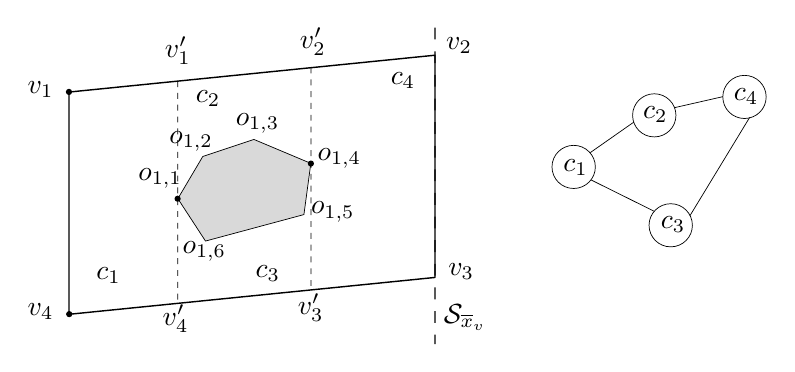
\begin{tikzpicture}[y=0.80pt, x=0.80pt, yscale=-\globalscale, xscale=\globalscale, inner sep=0pt, outer sep=0pt]
\path[draw=black,line join=round,line width=0.512pt] (18.6584,29.4063) -- (183.9870,12.7587) -- (183.9870,113.1380) -- (18.6584,129.7850) -- (18.6584,29.4063) -- cycle;

\path[draw=black,fill=black,line join=round,line width=0.512pt] (18.6440,29.3336) ellipse (0.0301cm and 0.0301cm);

\path[draw=black,fill=cD9D9D9,line join=round,line width=0.256pt] (67.8359,77.5466) -- (79.1010,58.4826) -- (102.1880,50.7973) -- (127.8940,61.6068) -- (124.7750,84.7435) -- (80.3210,96.7018) -- (67.8359,77.5466) -- cycle;

\path[draw=black,fill=black,line join=round,line width=0.512pt] (18.7578,128.6400) .. controls (19.3461,128.6400) and (19.8230,129.1170) .. (19.8230,129.7050) .. controls (19.8230,130.2930) and (19.3461,130.7700) .. (18.7578,130.7700) .. controls (18.1694,130.7700) and (17.6925,130.2930) .. (17.6925,129.7050) .. controls (17.6925,129.1170) and (18.1694,128.6400) .. (18.7578,128.6400) -- cycle;

\path[cm={{1.0,0.0,0.0,1.0,(0.0,32.0)}}] (0.0000,0.0000) node[above right] () {$v_1$};

\path[cm={{1.0,0.0,0.0,1.0,(0.0,132.0)}}] (0.0000,0.0000) node[above right] () {$v_4$};

\path[cm={{1.0,0.0,0.0,1.0,(189.0,12.0)}}] (0.0000,0.0000) node[above right] () {$v_2$};

\path[cm={{1.0,0.0,0.0,1.0,(190.0,114.0)}}] (0.0000,0.0000) node[above right] () {$v_3$};

\path[cm={{1.0,0.0,0.0,1.0,(50.0,73.0)}}] (0.0000,0.0000) node[above right] () {$o_{1,1}$};

\path[cm={{1.0,0.0,0.0,1.0,(64.0,56.0)}}] (0.0000,0.0000) node[above right] () {$o_{1,2}$};

\path[cm={{1.0,0.0,0.0,1.0,(94.0,48.0)}}] (0.0000,0.0000) node[above right] () {$o_{1,3}$};

\path[cm={{1.0,0.0,0.0,1.0,(131.0,64.0)}}] (0.0000,0.0000) node[above right] () {$o_{1,4}$};

\path[cm={{1.0,0.0,0.0,1.0,(128.0,88.0)}}] (0.0000,0.0000) node[above right] () {$o_{1,5}$};

\path[cm={{1.0,0.0,0.0,1.0,(70.0,106.0)}}] (0.0000,0.0000) node[above right] () {$o_{1,6}$};

\path[fill=black,line join=round,line width=0.256pt] (184.3070,10.9866) -- (184.3070,16.3199) -- (183.6670,16.3199) -- (183.6670,10.9866) -- (184.3070,10.9866) -- cycle(184.3070,21.6533) -- (184.3070,26.9866) -- (183.6670,26.9866) -- (183.6670,21.6533) -- (184.3070,21.6533) -- cycle(184.3070,32.3199) -- (184.3070,37.6533) -- (183.6670,37.6533) -- (183.6670,32.3199) -- (184.3070,32.3199) -- cycle(184.3070,42.9866) -- (184.3070,48.3199) -- (183.6670,48.3199) -- (183.6670,42.9866) -- (184.3070,42.9866) -- cycle(184.3070,53.6533) -- (184.3070,58.9866) -- (183.6670,58.9866) -- (183.6670,53.6533) -- (184.3070,53.6533) -- cycle(184.3070,64.3199) -- (184.3070,69.6533) -- (183.6670,69.6533) -- (183.6670,64.3199) -- (184.3070,64.3199) -- cycle(184.3070,74.9866) -- (184.3070,80.3199) -- (183.6670,80.3199) -- (183.6670,74.9866) -- (184.3070,74.9866) -- cycle(184.3070,85.6533) -- (184.3070,90.9866) -- (183.6670,90.9866) -- (183.6670,85.6533) -- (184.3070,85.6533) -- cycle(184.3070,96.3199) -- (184.3070,101.6530) -- (183.6670,101.6530) -- (183.6670,96.3199) -- (184.3070,96.3199) -- cycle(184.3070,106.9870) -- (184.3070,112.3200) -- (183.6670,112.3200) -- (183.6670,106.9870) -- (184.3070,106.9870) -- cycle(184.3070,117.6530) -- (184.3070,122.9870) -- (183.6670,122.9870) -- (183.6670,117.6530) -- (184.3070,117.6530) -- cycle(184.3070,128.3200) -- (184.3070,133.6530) -- (183.6670,133.6530) -- (183.6670,128.3200) -- (184.3070,128.3200) -- cycle(184.3070,138.9870) -- (184.3070,143.2150) -- (183.6670,143.2150) -- (183.6670,138.9870) -- (184.3070,138.9870) -- cycle(184.3070,0.3199) -- (184.3070,5.6533) -- (183.6670,5.6533) -- (183.6670,0.3199) -- (184.3070,0.3199) -- cycle;

\path[fill=black,line join=round,line width=0.256pt] (67.9514,29.7995) -- (67.9514,32.4661) -- (67.6314,32.4661) -- (67.6314,29.7995) -- (67.9514,29.7995) -- cycle(67.9514,35.1328) -- (67.9514,37.7995) -- (67.6314,37.7995) -- (67.6314,35.1328) -- (67.9514,35.1328) -- cycle(67.9514,40.4661) -- (67.9514,43.1328) -- (67.6314,43.1328) -- (67.6314,40.4661) -- (67.9514,40.4661) -- cycle(67.9514,45.7995) -- (67.9514,48.4661) -- (67.6314,48.4661) -- (67.6314,45.7995) -- (67.9514,45.7995) -- cycle(67.9514,51.1328) -- (67.9514,53.7995) -- (67.6314,53.7995) -- (67.6314,51.1328) -- (67.9514,51.1328) -- cycle(67.9514,56.4661) -- (67.9514,59.1328) -- (67.6314,59.1328) -- (67.6314,56.4661) -- (67.9514,56.4661) -- cycle(67.9514,61.7995) -- (67.9514,64.4661) -- (67.6314,64.4661) -- (67.6314,61.7995) -- (67.9514,61.7995) -- cycle(67.9514,67.1328) -- (67.9514,69.7995) -- (67.6314,69.7995) -- (67.6314,67.1328) -- (67.9514,67.1328) -- cycle(67.9514,72.4661) -- (67.9514,75.1328) -- (67.6314,75.1328) -- (67.6314,72.4661) -- (67.9514,72.4661) -- cycle(67.9514,77.7995) -- (67.9514,80.4661) -- (67.6314,80.4661) -- (67.6314,77.7995) -- (67.9514,77.7995) -- cycle(67.9514,83.1328) -- (67.9514,85.7995) -- (67.6314,85.7995) -- (67.6314,83.1328) -- (67.9514,83.1328) -- cycle(67.9514,88.4661) -- (67.9514,91.1328) -- (67.6314,91.1328) -- (67.6314,88.4661) -- (67.9514,88.4661) -- cycle(67.9514,93.7995) -- (67.9514,96.4661) -- (67.6314,96.4661) -- (67.6314,93.7995) -- (67.9514,93.7995) -- cycle(67.9514,99.1328) -- (67.9514,101.7990) -- (67.6314,101.7990) -- (67.6314,99.1328) -- (67.9514,99.1328) -- cycle(67.9514,104.4660) -- (67.9514,107.1330) -- (67.6314,107.1330) -- (67.6314,104.4660) -- (67.9514,104.4660) -- cycle(67.9514,109.7990) -- (67.9514,112.4660) -- (67.6314,112.4660) -- (67.6314,109.7990) -- (67.9514,109.7990) -- cycle(67.9514,115.1330) -- (67.9514,117.7990) -- (67.6314,117.7990) -- (67.6314,115.1330) -- (67.9514,115.1330) -- cycle(67.9514,120.4660) -- (67.9514,123.1330) -- (67.6314,123.1330) -- (67.6314,120.4660) -- (67.9514,120.4660) -- cycle(67.9514,24.4661) -- (67.9514,27.1328) -- (67.6314,27.1328) -- (67.6314,24.4661) -- (67.9514,24.4661) -- cycle;



\path[draw=black,fill=black,line join=round,line width=0.512pt] (67.7196,76.5121) .. controls (68.3080,76.5121) and (68.7849,76.9890) .. (68.7849,77.5773) .. controls (68.7849,78.1656) and (68.3080,78.6426) .. (67.7196,78.6426) .. controls (67.1313,78.6426) and (66.6544,78.1656) .. (66.6544,77.5773) .. controls (66.6544,76.9890) and (67.1313,76.5121) .. (67.7196,76.5121) -- cycle;

\path[fill=black,line join=round,line width=0.256pt] (128.1570,23.6663) -- (128.1570,26.3329) -- (127.8370,26.3329) -- (127.8370,23.6663) -- (128.1570,23.6663) -- cycle(128.1570,28.9996) -- (128.1570,31.6663) -- (127.8370,31.6663) -- (127.8370,28.9996) -- (128.1570,28.9996) -- cycle(128.1570,34.3329) -- (128.1570,36.9996) -- (127.8370,36.9996) -- (127.8370,34.3329) -- (128.1570,34.3329) -- cycle(128.1570,39.6663) -- (128.1570,42.3329) -- (127.8370,42.3329) -- (127.8370,39.6663) -- (128.1570,39.6663) -- cycle(128.1570,44.9996) -- (128.1570,47.6663) -- (127.8370,47.6663) -- (127.8370,44.9996) -- (128.1570,44.9996) -- cycle(128.1570,50.3329) -- (128.1570,52.9996) -- (127.8370,52.9996) -- (127.8370,50.3329) -- (128.1570,50.3329) -- cycle(128.1570,55.6663) -- (128.1570,58.3329) -- (127.8370,58.3329) -- (127.8370,55.6663) -- (128.1570,55.6663) -- cycle(128.1570,60.9996) -- (128.1570,63.6663) -- (127.8370,63.6663) -- (127.8370,60.9996) -- (128.1570,60.9996) -- cycle(128.1570,66.3329) -- (128.1570,68.9996) -- (127.8370,68.9996) -- (127.8370,66.3329) -- (128.1570,66.3329) -- cycle(128.1570,71.6663) -- (128.1570,74.3329) -- (127.8370,74.3329) -- (127.8370,71.6663) -- (128.1570,71.6663) -- cycle(128.1570,76.9996) -- (128.1570,79.6663) -- (127.8370,79.6663) -- (127.8370,76.9996) -- (128.1570,76.9996) -- cycle(128.1570,82.3329) -- (128.1570,84.9996) -- (127.8370,84.9996) -- (127.8370,82.3329) -- (128.1570,82.3329) -- cycle(128.1570,87.6663) -- (128.1570,90.3329) -- (127.8370,90.3329) -- (127.8370,87.6663) -- (128.1570,87.6663) -- cycle(128.1570,92.9996) -- (128.1570,95.6663) -- (127.8370,95.6663) -- (127.8370,92.9996) -- (128.1570,92.9996) -- cycle(128.1570,98.3329) -- (128.1570,101.0000) -- (127.8370,101.0000) -- (127.8370,98.3329) -- (128.1570,98.3329) -- cycle(128.1570,103.6660) -- (128.1570,106.3330) -- (127.8370,106.3330) -- (127.8370,103.6660) -- (128.1570,103.6660) -- cycle(128.1570,109.0000) -- (128.1570,111.6660) -- (127.8370,111.6660) -- (127.8370,109.0000) -- (128.1570,109.0000) -- cycle(128.1570,114.3330) -- (128.1570,117.0000) -- (127.8370,117.0000) -- (127.8370,114.3330) -- (128.1570,114.3330) -- cycle(128.1570,18.3329) -- (128.1570,20.9996) -- (127.8370,20.9996) -- (127.8370,18.3329) -- (128.1570,18.3329) -- cycle;



\path[draw=black,fill=black,line join=round,line width=0.512pt] (127.9250,60.6303) .. controls (128.5130,60.6303) and (128.9900,61.1072) .. (128.9900,61.6955) .. controls (128.9900,62.2838) and (128.5130,62.7607) .. (127.9250,62.7607) .. controls (127.3370,62.7607) and (126.8600,62.2838) .. (126.8600,61.6955) .. controls (126.8600,61.1072) and (127.3370,60.6303) .. (127.9250,60.6303) -- cycle;



\path[cm={{1.0,0.0,0.0,1.0,(188.0,137.0)}}] (0.0000,0.0000) node[above right] () {$\mathcal{S}_{\overline{x}_v}$};



\path[cm={{1.0,0.0,0.0,1.0,(62.0,17.0)}}] (0.0000,0.0000) node[above right] () {$v_1'$};



\path[cm={{1.0,0.0,0.0,1.0,(61.0,138.0)}}] (0.0000,0.0000) node[above right] () {$v_4'$};



\path[cm={{1.0,0.0,0.0,1.0,(123.0,13.0)}}] (0.0000,0.0000) node[above right] () {$v_2'$};



\path[cm={{1.0,0.0,0.0,1.0,(122.0,133.0)}}] (0.0000,0.0000) node[above right] () {$v_3'$};



\path[draw=black,line join=round,line width=0.256pt] (323.7740,21.8583) .. controls (329.1820,21.8583) and (333.5650,26.2197) .. (333.5650,31.6000) .. controls (333.5650,36.9802) and (329.1820,41.3417) .. (323.7740,41.3417) .. controls (318.3660,41.3417) and (313.9820,36.9802) .. (313.9820,31.6000) .. controls (313.9820,26.2197) and (318.3660,21.8583) .. (323.7740,21.8583) -- cycle;



\path[cm={{1.0,0.0,0.0,1.0,(319.0,35.0)}}] (0.0000,0.0000) node[above right] () {$c_4$};



\path[cm={{1.0,0.0,0.0,1.0,(31.0,116.0)}}] (0.0000,0.0000) node[above right] () {$c_1$};



\path[cm={{1.0,0.0,0.0,1.0,(76.0,36.0)}}] (0.0000,0.0000) node[above right] () {$c_2$};



\path[cm={{1.0,0.0,0.0,1.0,(164.0,28.0)}}] (0.0000,0.0000) node[above right] () {$c_4$};



\path[cm={{1.0,0.0,0.0,1.0,(103.0,115.0)}}] (0.0000,0.0000) node[above right] () {$c_3$};



\path[draw=black,line join=round,line width=0.256pt] (246.6150,53.4698) .. controls (252.0230,53.4698) and (256.4060,57.8313) .. (256.4060,63.2115) .. controls (256.4060,68.5917) and (252.0230,72.9532) .. (246.6150,72.9532) .. controls (241.2070,72.9532) and (236.8230,68.5917) .. (236.8230,63.2115) .. controls (236.8230,57.8313) and (241.2070,53.4698) .. (246.6150,53.4698) -- cycle;



\path[cm={{1.0,0.0,0.0,1.0,(242.0,67.0)}}] (0.0000,0.0000) node[above right] () {$c_1$};



\path[draw=black,line join=round,line width=0.256pt] (290.4520,79.8348) .. controls (295.8590,79.8348) and (300.2430,84.1964) .. (300.2430,89.5765) .. controls (300.2430,94.9568) and (295.8590,99.3182) .. (290.4520,99.3182) .. controls (285.0440,99.3182) and (280.6600,94.9568) .. (280.6600,89.5765) .. controls (280.6600,84.1964) and (285.0440,79.8348) .. (290.4520,79.8348) -- cycle;



\path[cm={{1.0,0.0,0.0,1.0,(286.0,93.0)}}] (0.0000,0.0000) node[above right] () {$c_3$};



\path[draw=black,line join=round,line width=0.256pt] (283.0240,30.1792) .. controls (288.4320,30.1792) and (292.8160,34.5407) .. (292.8160,39.9209) .. controls (292.8160,45.3011) and (288.4320,49.6626) .. (283.0240,49.6626) .. controls (277.6160,49.6626) and (273.2330,45.3011) .. (273.2330,39.9209) .. controls (273.2330,34.5407) and (277.6160,30.1792) .. (283.0240,30.1792) -- cycle;



\path[cm={{1.0,0.0,0.0,1.0,(278.0,43.0)}}] (0.0000,0.0000) node[above right] () {$c_2$};



\path[draw=black,line join=round,line width=0.256pt] (254.5720,69.1411) -- (283.1050,83.3010);



\path[draw=black,line join=round,line width=0.256pt] (254.0910,56.7695) -- (273.7710,42.9828);



\path[draw=black,line join=round,line width=0.256pt] (292.1050,36.4653) -- (314.0520,31.4699);

\path[draw=black,line join=round,line width=0.256pt] (326.1050,40.8653) -- (299.1050,85.3010);



\end{tikzpicture}


  \caption[Result of the boustrophedon decomposition]{The final step of the boustrophedon decomposition, where the sweeping line $\mathcal{S}_{\lambda}$ encounters the final point of its domain $\overline{x}_v$. The decomposition results in four cells. To determine the order of the coverage tour, the methodology is to  visit the adjacency graph.}
  \label{fig:bcd4}
\end{figure}
In \fref{fig:bcd3}{Figure}, $\mathcal{S}_\lambda$ sweeps the space from $\lambda=\underline{x}_v$ in \fref{fig:bcd2}{Figure} up to $\lambda=x_{o_{1,1}}$. At this latter lambda, $\mathcal{S}_{x_{o_{1,1}}}$ encounters a change in connectivity ($\mathcal{S}^v_{x_{o_{1,1}}}$ forms two disconnected slices). The decomposition methodology builds two new cells $c_2,c_3$, and adds these cells to the adjacency graph. $\mathcal{S}_\lambda$ encounters another change in connectivity at $\lambda=x_{o_{1,4}}$ ($\mathcal{S}^v_{x_{o_{1,4}}}$ is again one connected slice). This latter is different from the previous: the cells are merged with forming a new cell $c_4$. The coverage tour is then a visit through the adjacency graph, resulting in the coverage order $c_1,c_2,c_4$, and finally $c_3$. 

In summary, the methodology iterates through the environment with $\mathcal{S}^v_{\lambda}$ in \fref{fig:bcd2}{Figure}. When the connectivity of $\mathcal{S}^v_{\lambda}$ increases in \fref{fig:bcd3}{Figure}, it closes a cell and opens two new cells--the literature~\citep{choset2000exact,choset2005principles} refers to these cells as ceiling and floor cells (for $c_2$ and $c_3$ in~\fref{fig:bcd4}{Figure} respectively). When the connectivity decreases back in \fref{fig:bcd4}{Figure}, the two opened cells are closed, and a new one is opened. The overall complexity is $O(n\log{n})$ with $n:=|v|+\sum_{i=1}^{|o|}|o_i|$ the total number of vertices~\citep{choset2000exact}. Indeed, for polygonal environments, it is enough to verify the change in connectivity by iterating the vertices and visit the constructed adjacency graph to find the coverage order.

\subsection{Coverage motion generation}\findex{coverage motion}
\label{sec:cov-motion}

Once we delimited the coverage and obstacles spaces into appropriate cells, we need to define the tour that travels through all the points in the cells--the coverage motion. A classical approach for the coverage motion in the literature is to travel back and forth. We saw in~\fref{cp:soa}{Chapter} and discussed briefly at the beginning of~\fref{sec:cov-path-plan}{Section} that this is termed the boustrophedon motion. We propose a slight variation of this motion for our problem, which we introduced with the intuitive path in~\fref{sec:path-wise}{Section} in~\fref{fig:bm-like_pb}{Figure}. The variation called the boustrophedon-like motion optimizes the turns of the aerial robot flying. The past literature analyzes broadly turns optimizations in the coverage for both mobile~\citep{huang2001optimal} and aerial robots~\citep{artemenko2016energy,li2011coverage}. The problem is that mobile robots are often subject to various constraints, including the turning radius. The original boustrophedon motion has edges parallel to the polygon where a mobile robot might have to slow to perform the turn. For instance, a lawnmower mobile robot would have to drive outside the path to turn efficiently~\citep{huang2001optimal}. An aerial robot traveling the boustrophedon motion might have to follow a greedy path planning algorithm instead or travel an additional turning maneuver such as a curlicue orbit~\citep{xu2011optimal,xu2014efficient}. To this end, the boustrophedon-like motion in~\fref{sec:path-wise}{Section} considerably smooths the turns. Given two following back and forth parallel lines in the original version, ours connects these lines using a semi-circle of a given radius rather than connecting them with additional lines. We illustrate how we cover the cell $c_1$ in~\fref{fig:bcd4}{Figure} using the boustrophedon-like motion in~\fref{fig:bm}{Figure}. 
\begin{figure}[h]
  \centering
  \fontfamily{phv}\selectfont
  
\definecolor{cD9D9D9}{RGB}{217,217,217}
\small

\def \globalscale {1.000000}
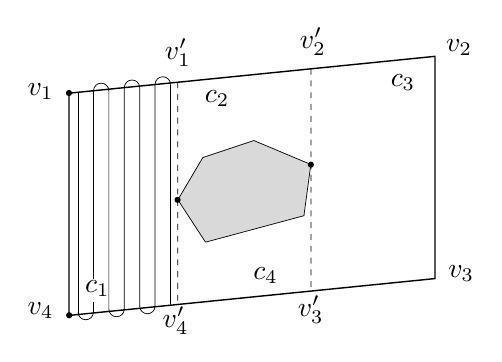
\begin{tikzpicture}[y=0.80pt, x=0.80pt, yscale=-\globalscale, xscale=\globalscale, inner sep=0pt, outer sep=0pt]
\path[draw=black,line join=round,line width=0.512pt] (18.6584,24.0976) -- (183.9870,7.4501) -- (183.9870,107.8290) -- (18.6584,124.4770) -- (18.6584,24.0976) -- cycle;



\path[draw=black,fill=black,line join=round,line width=0.512pt] (18.6440,22.9597) .. controls (19.2323,22.9597) and (19.7092,23.4366) .. (19.7092,24.0249) .. controls (19.7092,24.6132) and (19.2323,25.0901) .. (18.6440,25.0901) .. controls (18.0556,25.0901) and (17.5787,24.6132) .. (17.5787,24.0249) .. controls (17.5787,23.4366) and (18.0556,22.9597) .. (18.6440,22.9597) -- cycle;



\path[draw=black,fill=cD9D9D9,line join=round,line width=0.256pt] (67.8359,72.2380) -- (79.1010,53.1740) -- (102.1880,45.4887) -- (127.8940,56.2981) -- (124.7750,79.4348) -- (80.3210,91.3931) -- (67.8359,72.2380) -- cycle;



\path[draw=black,fill=black,line join=round,line width=0.512pt] (18.7578,123.3310) .. controls (19.3461,123.3310) and (19.8230,123.8080) .. (19.8230,124.3960) .. controls (19.8230,124.9850) and (19.3461,125.4610) .. (18.7578,125.4610) .. controls (18.1694,125.4610) and (17.6925,124.9850) .. (17.6925,124.3960) .. controls (17.6925,123.8080) and (18.1694,123.3310) .. (18.7578,123.3310) -- cycle;



\path[cm={{1.0,0.0,0.0,1.0,(0.0,27.0)}}] (0.0000,0.0000) node[above right] () {$v_1$};



\path[cm={{1.0,0.0,0.0,1.0,(0.0,126.0)}}] (0.0000,0.0000) node[above right] () {$v_4$};



\path[cm={{1.0,0.0,0.0,1.0,(189.0,7.0)}}] (0.0000,0.0000) node[above right] () {$v_2$};



\path[cm={{1.0,0.0,0.0,1.0,(190.0,109.0)}}] (0.0000,0.0000) node[above right] () {$v_3$};



\path[fill=black,line join=round,line width=0.256pt] (67.9514,24.4908) -- (67.9514,27.1574) -- (67.6314,27.1574) -- (67.6314,24.4908) -- (67.9514,24.4908) -- cycle(67.9514,29.8241) -- (67.9514,32.4908) -- (67.6314,32.4908) -- (67.6314,29.8241) -- (67.9514,29.8241) -- cycle(67.9514,35.1574) -- (67.9514,37.8241) -- (67.6314,37.8241) -- (67.6314,35.1574) -- (67.9514,35.1574) -- cycle(67.9514,40.4908) -- (67.9514,43.1574) -- (67.6314,43.1574) -- (67.6314,40.4908) -- (67.9514,40.4908) -- cycle(67.9514,45.8241) -- (67.9514,48.4908) -- (67.6314,48.4908) -- (67.6314,45.8241) -- (67.9514,45.8241) -- cycle(67.9514,51.1574) -- (67.9514,53.8241) -- (67.6314,53.8241) -- (67.6314,51.1574) -- (67.9514,51.1574) -- cycle(67.9514,56.4908) -- (67.9514,59.1574) -- (67.6314,59.1574) -- (67.6314,56.4908) -- (67.9514,56.4908) -- cycle(67.9514,61.8241) -- (67.9514,64.4908) -- (67.6314,64.4908) -- (67.6314,61.8241) -- (67.9514,61.8241) -- cycle(67.9514,67.1574) -- (67.9514,69.8241) -- (67.6314,69.8241) -- (67.6314,67.1574) -- (67.9514,67.1574) -- cycle(67.9514,72.4908) -- (67.9514,75.1574) -- (67.6314,75.1574) -- (67.6314,72.4908) -- (67.9514,72.4908) -- cycle(67.9514,77.8241) -- (67.9514,80.4908) -- (67.6314,80.4908) -- (67.6314,77.8241) -- (67.9514,77.8241) -- cycle(67.9514,83.1574) -- (67.9514,85.8241) -- (67.6314,85.8241) -- (67.6314,83.1574) -- (67.9514,83.1574) -- cycle(67.9514,88.4908) -- (67.9514,91.1574) -- (67.6314,91.1574) -- (67.6314,88.4908) -- (67.9514,88.4908) -- cycle(67.9514,93.8241) -- (67.9514,96.4908) -- (67.6314,96.4908) -- (67.6314,93.8241) -- (67.9514,93.8241) -- cycle(67.9514,99.1574) -- (67.9514,101.8240) -- (67.6314,101.8240) -- (67.6314,99.1574) -- (67.9514,99.1574) -- cycle(67.9514,104.4910) -- (67.9514,107.1570) -- (67.6314,107.1570) -- (67.6314,104.4910) -- (67.9514,104.4910) -- cycle(67.9514,109.8240) -- (67.9514,112.4910) -- (67.6314,112.4910) -- (67.6314,109.8240) -- (67.9514,109.8240) -- cycle(67.9514,115.1570) -- (67.9514,117.8240) -- (67.6314,117.8240) -- (67.6314,115.1570) -- (67.9514,115.1570) -- cycle(67.9514,19.1574) -- (67.9514,21.8241) -- (67.6314,21.8241) -- (67.6314,19.1574) -- (67.9514,19.1574) -- cycle;



\path[draw=black,fill=black,line join=round,line width=0.512pt] (67.7196,71.2034) .. controls (68.3080,71.2034) and (68.7849,71.6804) .. (68.7849,72.2687) .. controls (68.7849,72.8570) and (68.3080,73.3339) .. (67.7196,73.3339) .. controls (67.1313,73.3339) and (66.6544,72.8570) .. (66.6544,72.2687) .. controls (66.6544,71.6804) and (67.1313,71.2034) .. (67.7196,71.2034) -- cycle;



\path[fill=black,line join=round,line width=0.256pt] (128.1570,18.3576) -- (128.1570,21.0243) -- (127.8370,21.0243) -- (127.8370,18.3576) -- (128.1570,18.3576) -- cycle(128.1570,23.6910) -- (128.1570,26.3576) -- (127.8370,26.3576) -- (127.8370,23.6910) -- (128.1570,23.6910) -- cycle(128.1570,29.0243) -- (128.1570,31.6910) -- (127.8370,31.6910) -- (127.8370,29.0243) -- (128.1570,29.0243) -- cycle(128.1570,34.3576) -- (128.1570,37.0243) -- (127.8370,37.0243) -- (127.8370,34.3576) -- (128.1570,34.3576) -- cycle(128.1570,39.6910) -- (128.1570,42.3576) -- (127.8370,42.3576) -- (127.8370,39.6910) -- (128.1570,39.6910) -- cycle(128.1570,45.0243) -- (128.1570,47.6910) -- (127.8370,47.6910) -- (127.8370,45.0243) -- (128.1570,45.0243) -- cycle(128.1570,50.3576) -- (128.1570,53.0243) -- (127.8370,53.0243) -- (127.8370,50.3576) -- (128.1570,50.3576) -- cycle(128.1570,55.6910) -- (128.1570,58.3576) -- (127.8370,58.3576) -- (127.8370,55.6910) -- (128.1570,55.6910) -- cycle(128.1570,61.0243) -- (128.1570,63.6910) -- (127.8370,63.6910) -- (127.8370,61.0243) -- (128.1570,61.0243) -- cycle(128.1570,66.3576) -- (128.1570,69.0243) -- (127.8370,69.0243) -- (127.8370,66.3576) -- (128.1570,66.3576) -- cycle(128.1570,71.6910) -- (128.1570,74.3576) -- (127.8370,74.3576) -- (127.8370,71.6910) -- (128.1570,71.6910) -- cycle(128.1570,77.0243) -- (128.1570,79.6910) -- (127.8370,79.6910) -- (127.8370,77.0243) -- (128.1570,77.0243) -- cycle(128.1570,82.3576) -- (128.1570,85.0243) -- (127.8370,85.0243) -- (127.8370,82.3576) -- (128.1570,82.3576) -- cycle(128.1570,87.6910) -- (128.1570,90.3576) -- (127.8370,90.3576) -- (127.8370,87.6910) -- (128.1570,87.6910) -- cycle(128.1570,93.0243) -- (128.1570,95.6910) -- (127.8370,95.6910) -- (127.8370,93.0243) -- (128.1570,93.0243) -- cycle(128.1570,98.3576) -- (128.1570,101.0240) -- (127.8370,101.0240) -- (127.8370,98.3576) -- (128.1570,98.3576) -- cycle(128.1570,103.6910) -- (128.1570,106.3580) -- (127.8370,106.3580) -- (127.8370,103.6910) -- (128.1570,103.6910) -- cycle(128.1570,109.0240) -- (128.1570,111.6910) -- (127.8370,111.6910) -- (127.8370,109.0240) -- (128.1570,109.0240) -- cycle(128.1570,13.0243) -- (128.1570,15.6910) -- (127.8370,15.6910) -- (127.8370,13.0243) -- (128.1570,13.0243) -- cycle;



\path[draw=black,fill=black,line join=round,line width=0.512pt] (127.9250,55.3216) .. controls (128.5130,55.3216) and (128.9900,55.7985) .. (128.9900,56.3868) .. controls (128.9900,56.9751) and (128.5130,57.4521) .. (127.9250,57.4521) .. controls (127.3370,57.4521) and (126.8600,56.9751) .. (126.8600,56.3868) .. controls (126.8600,55.7985) and (127.3370,55.3216) .. (127.9250,55.3216) -- cycle;



\path[cm={{1.0,0.0,0.0,1.0,(62.0,12.0)}}] (0.0000,0.0000) node[above right] () {$v_1'$};



\path[cm={{1.0,0.0,0.0,1.0,(61.0,133.0)}}] (0.0000,0.0000) node[above right] () {$v_4'$};



\path[cm={{1.0,0.0,0.0,1.0,(123.0,7.0)}}] (0.0000,0.0000) node[above right] () {$v_2'$};



\path[cm={{1.0,0.0,0.0,1.0,(122.0,128.0)}}] (0.0000,0.0000) node[above right] () {$v_3'$};



\path[cm={{1.0,0.0,0.0,1.0,(26.0,116.0)}}] (0.0000,0.0000) node[above right] () {$c_1$};



\path[cm={{1.0,0.0,0.0,1.0,(80.0,30.0)}}] (0.0000,0.0000) node[above right] () {$c_2$};



\path[cm={{1.0,0.0,0.0,1.0,(164.0,23.0)}}] (0.0000,0.0000) node[above right] () {$c_3$};



\path[cm={{1.0,0.0,0.0,1.0,(102.0,110.0)}}] (0.0000,0.0000) node[above right] () {$c_4$};



\path[draw=black,line join=round,line width=0.256pt] (22.7526,23.5645) -- (22.7526,123.6130);



\path[draw=black,line join=round,line width=0.256pt] (29.7125,23.0445) .. controls (29.7125,21.1226) and (31.2706,19.5645) .. (33.1925,19.5645) .. controls (35.1143,19.5645) and (36.6724,21.1226) .. (36.6724,23.0445);



\path[draw=black,line join=round,line width=0.256pt] (29.7125,122.9440) .. controls (29.7125,124.8660) and (28.1545,126.4240) .. (26.2326,126.4240) .. controls (24.3106,126.4240) and (22.7526,124.8660) .. (22.7526,122.9440);



\path[draw=black,line join=round,line width=0.256pt] (29.7125,22.9673) -- (29.7125,108.1990);



\path[draw=black,line join=round,line width=0.256pt] (29.7125,118.2240) -- (29.7125,123.0150);



\path[draw=black,line join=round,line width=0.256pt] (36.6723,23.0215) -- (36.6724,121.6680);



\path[draw=black,line join=round,line width=0.256pt] (43.6324,121.5940) .. controls (43.6324,123.5160) and (42.0743,125.0740) .. (40.1524,125.0740) .. controls (38.2305,125.0740) and (36.6724,123.5160) .. (36.6724,121.5940);



\path[draw=black,line join=round,line width=0.256pt] (43.6321,21.3950) -- (43.6324,121.6410);



\path[draw=black,line join=round,line width=0.256pt] (43.6322,21.6181) .. controls (43.6322,19.6963) and (45.1903,18.1383) .. (47.1122,18.1383) .. controls (49.0340,18.1383) and (50.5922,19.6963) .. (50.5922,21.6181);



\path[draw=black,line join=round,line width=0.256pt] (50.5919,21.5756) -- (50.5920,120.4230);



\path[draw=black,line join=round,line width=0.256pt] (57.5519,120.2440) .. controls (57.5519,122.1660) and (55.9938,123.7240) .. (54.0719,123.7240) .. controls (52.1499,123.7240) and (50.5919,122.1660) .. (50.5919,120.2440);



\path[draw=black,line join=round,line width=0.256pt] (57.5517,19.9092) -- (57.5519,120.2560);



\path[draw=black,line join=round,line width=0.256pt] (57.5518,20.1484) .. controls (57.5518,18.2265) and (59.1098,16.6685) .. (61.0317,16.6685) .. controls (62.9536,16.6685) and (64.5117,18.2265) .. (64.5117,20.1484);



\path[draw=black,line join=round,line width=0.256pt] (64.5116,20.1943) -- (64.5115,119.6430);




\end{tikzpicture}


  \caption[Boustrophedon-like motion covering a cell]{The boustrophedon-like motion covering the cell $c_1$, composed of back and forth parallel lines and circles connecting them of radius half the ideal coverage distance.}
  \label{fig:bm}
\end{figure}
The remaining cells are covered in the same manner. The overall coverage is achieved by visiting the cells in the appropriate order derived in the previous section ($c_1,c_2,c_4,$ and $c_3$).

Let us assume for an instant that the turning radius in~\fref{pb:cov-pb}{Problem} is not given. Let us further assume that the aerial robot can overfly the boundaries of the polygons $v$ and $o_i$ for the turns. The methodology that outputs the plan $\Gamma$ that covers $\mathcal{Q}^v$ with boustrophedon-like motion is to build four paths:
\begin{enumerate*}[label={(\alph*)},font={\textit}]
  \item the line $\varphi_1$ from \fref{fig:bm-like_pb}{Figure} parallel to the edge formed by vertices $v_1$ and $v_4$,
  \item the circle $\varphi_2$ with the center laying on the edge formed by vertices $v_4$ and $v_3$,
  \item the line $\varphi_3$ parallel to $\varphi_1$ that connects the right side of $\varphi_2$ and extends up to the left side of $\varphi_4$, and
  \item the circle $\varphi_4$ whose center is on the edge formed by vertices $v_1$ and $v_2$.
\end{enumerate*}
The remaining paths $\varphi_5,\varphi_6,\dots$ are formed similarly. To evaluate the radius of the circles, let us assume the ideal distance between the vertical lines in the motion (the lines $\varphi_1,\varphi_3,\varphi_5,\dots$) is a given constant. Then the radius in the plan (the circles $\varphi_2,\varphi_4,\varphi_6,\dots$) is half the ideal distance. We can change the radius of the circles and thus alter the quality of the coverage accordingly. Indeed our planning approach consists of generating an initial plan that can be changed in a replanning phase using an optimal control technique in \fref{sec:output-mpc}{Section} with the aerial robot being subject to uncertainty and external interferences in flight.

Although the turns are considerably smoothed with the plan containing the boustrophedon-like motion, they are still impractical for fixed-wing aerial robots with the turning radius exceeding the radius of these turns~\citep{dille2013efficient,xu2011optimal,xu2014efficient}. For this latter class of robots, we utilize the Zamboni-like motion. The Zamboni motion is often in the literature for fixed-wing aerial robots~\citep{ablavsky2000optimal,araujo2013multiple,majeed2019new}, and its name comes from the hockey arenas' ice maintenance machines~\citep{araujo2013multiple,dille2013efficient,ablavsky2000optimal}. They have a large turning radius like the aerial robots we study; hence they resurface the ice by sweeping distant lines first instead of adjacent lines in a back and forth motion (the boustrophedon or boustrophedon-like motions). 
\begin{figure}[h]
  \centering
  \fontfamily{phv}\selectfont
  
\definecolor{cD9D9D9}{RGB}{217,217,217}
\small

\def \globalscale {1.100000}
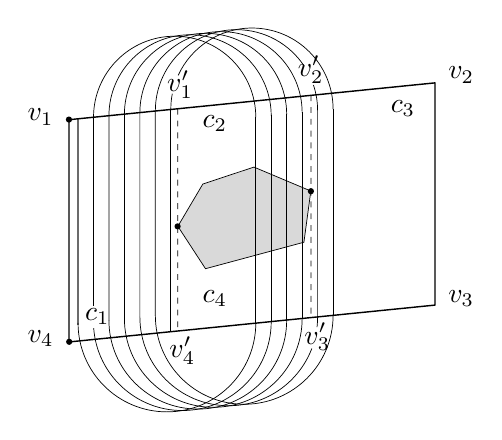
\begin{tikzpicture}[y=0.80pt, x=0.80pt, yscale=-\globalscale, xscale=\globalscale, inner sep=0pt, outer sep=0pt]
\path[draw=black,line join=round,line width=0.512pt] (18.6584,41.5752) -- (183.9870,24.9278) -- (183.9870,125.3070) -- (18.6584,141.9540) -- (18.6584,41.5752) -- cycle;



\path[draw=black,fill=black,line join=round,line width=0.512pt] (18.6440,40.4374) .. controls (19.2323,40.4374) and (19.7092,40.9143) .. (19.7092,41.5026) .. controls (19.7092,42.0909) and (19.2323,42.5679) .. (18.6440,42.5679) .. controls (18.0556,42.5679) and (17.5787,42.0909) .. (17.5787,41.5026) .. controls (17.5787,40.9143) and (18.0556,40.4374) .. (18.6440,40.4374) -- cycle;



\path[draw=black,fill=cD9D9D9,line join=round,line width=0.256pt] (67.8359,89.7156) -- (79.1010,70.6516) -- (102.1880,62.9663) -- (127.8940,73.7758) -- (124.7750,96.9125) -- (80.3210,108.8710) -- (67.8359,89.7156) -- cycle;



\path[draw=black,fill=black,line join=round,line width=0.512pt] (18.7578,140.8090) .. controls (19.3461,140.8090) and (19.8230,141.2860) .. (19.8230,141.8740) .. controls (19.8230,142.4620) and (19.3461,142.9390) .. (18.7578,142.9390) .. controls (18.1695,142.9390) and (17.6925,142.4620) .. (17.6925,141.8740) .. controls (17.6925,141.2860) and (18.1695,140.8090) .. (18.7578,140.8090) -- cycle;



\path[cm={{1.0,0.0,0.0,1.0,(0.0,44.0)}}] (0.0000,0.0000) node[above right] () {$v_1$};



\path[cm={{1.0,0.0,0.0,1.0,(0.0,144.0)}}] (0.0000,0.0000) node[above right] () {$v_4$};



\path[cm={{1.0,0.0,0.0,1.0,(190.0,25.0)}}] (0.0000,0.0000) node[above right] () {$v_2$};



\path[cm={{1.0,0.0,0.0,1.0,(190.0,126.0)}}] (0.0000,0.0000) node[above right] () {$v_3$};



\path[fill=black,line join=round,line width=0.256pt] (67.9514,41.9685) -- (67.9514,44.6352) -- (67.6314,44.6352) -- (67.6314,41.9685) -- (67.9514,41.9685) -- cycle(67.9514,47.3018) -- (67.9514,49.9685) -- (67.6314,49.9685) -- (67.6314,47.3018) -- (67.9514,47.3018) -- cycle(67.9514,52.6352) -- (67.9514,55.3018) -- (67.6314,55.3018) -- (67.6314,52.6352) -- (67.9514,52.6352) -- cycle(67.9514,57.9685) -- (67.9514,60.6352) -- (67.6314,60.6352) -- (67.6314,57.9685) -- (67.9514,57.9685) -- cycle(67.9514,63.3018) -- (67.9514,65.9685) -- (67.6314,65.9685) -- (67.6314,63.3018) -- (67.9514,63.3018) -- cycle(67.9514,68.6352) -- (67.9514,71.3018) -- (67.6314,71.3018) -- (67.6314,68.6352) -- (67.9514,68.6352) -- cycle(67.9514,73.9685) -- (67.9514,76.6352) -- (67.6314,76.6352) -- (67.6314,73.9685) -- (67.9514,73.9685) -- cycle(67.9514,79.3018) -- (67.9514,81.9685) -- (67.6314,81.9685) -- (67.6314,79.3018) -- (67.9514,79.3018) -- cycle(67.9514,84.6352) -- (67.9514,87.3018) -- (67.6314,87.3018) -- (67.6314,84.6352) -- (67.9514,84.6352) -- cycle(67.9514,89.9685) -- (67.9514,92.6352) -- (67.6314,92.6352) -- (67.6314,89.9685) -- (67.9514,89.9685) -- cycle(67.9514,95.3018) -- (67.9514,97.9685) -- (67.6314,97.9685) -- (67.6314,95.3018) -- (67.9514,95.3018) -- cycle(67.9514,100.6350) -- (67.9514,103.3020) -- (67.6314,103.3020) -- (67.6314,100.6350) -- (67.9514,100.6350) -- cycle(67.9514,105.9690) -- (67.9514,108.6350) -- (67.6314,108.6350) -- (67.6314,105.9690) -- (67.9514,105.9690) -- cycle(67.9514,111.3020) -- (67.9514,113.9690) -- (67.6314,113.9690) -- (67.6314,111.3020) -- (67.9514,111.3020) -- cycle(67.9514,116.6350) -- (67.9514,119.3020) -- (67.6314,119.3020) -- (67.6314,116.6350) -- (67.9514,116.6350) -- cycle(67.9514,121.9690) -- (67.9514,124.6350) -- (67.6314,124.6350) -- (67.6314,121.9690) -- (67.9514,121.9690) -- cycle(67.9514,127.3020) -- (67.9514,129.9690) -- (67.6314,129.9690) -- (67.6314,127.3020) -- (67.9514,127.3020) -- cycle(67.9514,132.6350) -- (67.9514,135.3020) -- (67.6314,135.3020) -- (67.6314,132.6350) -- (67.9514,132.6350) -- cycle(67.9514,36.6352) -- (67.9514,39.3018) -- (67.6314,39.3018) -- (67.6314,36.6352) -- (67.9514,36.6352) -- cycle;



\path[draw=black,fill=black,line join=round,line width=0.512pt] (67.7196,88.6812) .. controls (68.3079,88.6812) and (68.7849,89.1580) .. (68.7849,89.7464) .. controls (68.7849,90.3346) and (68.3079,90.8116) .. (67.7196,90.8116) .. controls (67.1313,90.8116) and (66.6544,90.3346) .. (66.6544,89.7464) .. controls (66.6544,89.1580) and (67.1313,88.6812) .. (67.7196,88.6812) -- cycle;



\path[fill=black,line join=round,line width=0.256pt] (128.1570,35.8352) -- (128.1570,38.5020) -- (127.8370,38.5020) -- (127.8370,35.8352) -- (128.1570,35.8352) -- cycle(128.1570,41.1686) -- (128.1570,43.8352) -- (127.8370,43.8352) -- (127.8370,41.1686) -- (128.1570,41.1686) -- cycle(128.1570,46.5020) -- (128.1570,49.1686) -- (127.8370,49.1686) -- (127.8370,46.5020) -- (128.1570,46.5020) -- cycle(128.1570,51.8352) -- (128.1570,54.5020) -- (127.8370,54.5020) -- (127.8370,51.8352) -- (128.1570,51.8352) -- cycle(128.1570,57.1686) -- (128.1570,59.8352) -- (127.8370,59.8352) -- (127.8370,57.1686) -- (128.1570,57.1686) -- cycle(128.1570,62.5020) -- (128.1570,65.1686) -- (127.8370,65.1686) -- (127.8370,62.5020) -- (128.1570,62.5020) -- cycle(128.1570,67.8352) -- (128.1570,70.5020) -- (127.8370,70.5020) -- (127.8370,67.8352) -- (128.1570,67.8352) -- cycle(128.1570,73.1686) -- (128.1570,75.8352) -- (127.8370,75.8352) -- (127.8370,73.1686) -- (128.1570,73.1686) -- cycle(128.1570,78.5020) -- (128.1570,81.1686) -- (127.8370,81.1686) -- (127.8370,78.5020) -- (128.1570,78.5020) -- cycle(128.1570,83.8352) -- (128.1570,86.5020) -- (127.8370,86.5020) -- (127.8370,83.8352) -- (128.1570,83.8352) -- cycle(128.1570,89.1686) -- (128.1570,91.8352) -- (127.8370,91.8352) -- (127.8370,89.1686) -- (128.1570,89.1686) -- cycle(128.1570,94.5020) -- (128.1570,97.1686) -- (127.8370,97.1686) -- (127.8370,94.5020) -- (128.1570,94.5020) -- cycle(128.1570,99.8352) -- (128.1570,102.5020) -- (127.8370,102.5020) -- (127.8370,99.8352) -- (128.1570,99.8352) -- cycle(128.1570,105.1690) -- (128.1570,107.8350) -- (127.8370,107.8350) -- (127.8370,105.1690) -- (128.1570,105.1690) -- cycle(128.1570,110.5020) -- (128.1570,113.1690) -- (127.8370,113.1690) -- (127.8370,110.5020) -- (128.1570,110.5020) -- cycle(128.1570,115.8350) -- (128.1570,118.5020) -- (127.8370,118.5020) -- (127.8370,115.8350) -- (128.1570,115.8350) -- cycle(128.1570,121.1690) -- (128.1570,123.8350) -- (127.8370,123.8350) -- (127.8370,121.1690) -- (128.1570,121.1690) -- cycle(128.1570,126.5020) -- (128.1570,129.1690) -- (127.8370,129.1690) -- (127.8370,126.5020) -- (128.1570,126.5020) -- cycle(128.1570,30.5020) -- (128.1570,33.1686) -- (127.8370,33.1686) -- (127.8370,30.5020) -- (128.1570,30.5020) -- cycle;



\path[draw=black,fill=black,line join=round,line width=0.512pt] (127.9250,72.7992) .. controls (128.5130,72.7992) and (128.9900,73.2762) .. (128.9900,73.8644) .. controls (128.9900,74.4527) and (128.5130,74.9297) .. (127.9250,74.9297) .. controls (127.3370,74.9297) and (126.8600,74.4527) .. (126.8600,73.8644) .. controls (126.8600,73.2762) and (127.3370,72.7992) .. (127.9250,72.7992) -- cycle;



\path[cm={{1.0,0.0,0.0,1.0,(63.0,32.0)}}] (0.0000,0.0000) node[above right] () {$v_1'$};



\path[cm={{1.0,0.0,0.0,1.0,(64.0,152.0)}}] (0.0000,0.0000) node[above right] () {$v_4'$};



\path[cm={{1.0,0.0,0.0,1.0,(122.0,25.0)}}] (0.0000,0.0000) node[above right] () {$v_2'$};



\path[cm={{1.0,0.0,0.0,1.0,(125.0,146.0)}}] (0.0000,0.0000) node[above right] () {$v_3'$};



\path[cm={{1.0,0.0,0.0,1.0,(26.0,134.0)}}] (0.0000,0.0000) node[above right] () {$c_1$};



\path[cm={{1.0,0.0,0.0,1.0,(79.0,47.0)}}] (0.0000,0.0000) node[above right] () {$c_2$};



\path[cm={{1.0,0.0,0.0,1.0,(164.0,40.0)}}] (0.0000,0.0000) node[above right] () {$c_3$};



\path[cm={{1.0,0.0,0.0,1.0,(79.0,126.0)}}] (0.0000,0.0000) node[above right] () {$c_4$};



\path[draw=black,line join=round,line width=0.256pt] (22.7526,41.0423) -- (22.7519,134.2950);



\path[draw=black,line join=round,line width=0.256pt] (29.7411,40.5077) .. controls (29.7411,20.2677) and (46.1500,3.8587) .. (66.3900,3.8587) .. controls (86.6300,3.8587) and (103.0390,20.2677) .. (103.0390,40.5077);



\path[draw=black,line join=round,line width=0.256pt] (103.0390,133.3880) .. controls (103.0390,155.5580) and (85.0663,173.5310) .. (62.8959,173.5310) .. controls (40.7255,173.5310) and (22.7528,155.5580) .. (22.7528,133.3880);



\path[draw=black,line join=round,line width=0.256pt] (29.7125,40.4449) -- (29.7125,125.6770);



\path[draw=black,line join=round,line width=0.256pt] (103.0390,40.4004) -- (103.0390,118.2310);



\path[draw=black,line join=round,line width=0.256pt] (103.0390,118.1180) -- (103.0390,133.5460);



\path[draw=black,line join=round,line width=0.256pt] (43.6892,38.8726) -- (43.6892,131.4200);



\path[draw=black,line join=round,line width=0.256pt] (50.6773,38.3545) -- (50.6775,130.7010);



\path[draw=black,line join=round,line width=0.256pt] (57.6657,37.6869) -- (57.6658,130.0340);



\path[draw=black,line join=round,line width=0.256pt] (64.6540,37.0723) -- (64.6540,137.1210);



\path[draw=black,line join=round,line width=0.256pt] (109.9990,132.7860) .. controls (109.9990,154.9570) and (92.0261,172.9290) .. (69.8557,172.9290) .. controls (48.6623,172.9290) and (31.3046,156.5070) .. (29.8162,135.6910);



\path[draw=black,line join=round,line width=0.256pt] (109.9990,39.5480) -- (109.9990,132.6940);



\path[draw=black,line join=round,line width=0.256pt] (36.7008,39.8515) .. controls (36.7008,19.6115) and (53.1098,3.2024) .. (73.3498,3.2024) .. controls (93.5898,3.2024) and (109.9990,19.6115) .. (109.9990,39.8515);



\path[draw=black,line join=round,line width=0.256pt] (36.7014,39.8069) -- (36.7008,132.2590);



\path[draw=black,line join=round,line width=0.256pt] (22.7526,41.0423) -- (22.7519,134.2950);



\path[draw=black,line join=round,line width=0.256pt] (116.9870,39.0512) -- (116.9870,132.1970);



\path[draw=black,line join=round,line width=0.256pt] (43.6891,39.2030) .. controls (43.6891,18.9630) and (60.0981,2.5540) .. (80.3381,2.5540) .. controls (100.5780,2.5540) and (116.9870,18.9630) .. (116.9870,39.2030);



\path[draw=black,line join=round,line width=0.256pt] (123.9750,38.2325) -- (123.9750,131.3780);



\path[draw=black,line join=round,line width=0.256pt] (50.6774,38.4309) .. controls (50.6774,18.1909) and (67.0864,1.7819) .. (87.3264,1.7819) .. controls (107.5660,1.7819) and (123.9750,18.1909) .. (123.9750,38.4309);



\path[draw=black,line join=round,line width=0.256pt] (116.9870,132.1240) .. controls (116.9870,154.2940) and (99.0144,172.2670) .. (76.8440,172.2670) .. controls (54.6736,172.2670) and (36.7008,154.2940) .. (36.7008,132.1240);



\path[draw=black,line join=round,line width=0.256pt] (123.9750,131.3240) .. controls (123.9750,153.4950) and (106.0030,171.4680) .. (83.8323,171.4680) .. controls (61.6619,171.4680) and (43.6891,153.4950) .. (43.6891,131.3240);



\path[draw=black,line join=round,line width=0.256pt] (130.9640,130.6190) .. controls (130.9640,132.1990) and (130.8720,133.7590) .. (130.6950,135.2920);



\path[draw=black,line join=round,line width=0.256pt] (128.3350,144.9360) .. controls (122.5690,160.0380) and (107.9470,170.7620) .. (90.8206,170.7620) .. controls (68.6502,170.7620) and (50.6774,152.7890) .. (50.6774,130.6190);



\path[draw=black,line join=round,line width=0.256pt] (130.9630,37.4865) -- (130.9640,130.6320);



\path[draw=black,line join=round,line width=0.256pt] (57.6657,37.5487) .. controls (57.6657,17.3087) and (74.0747,0.8997) .. (94.3147,0.8997) .. controls (107.1010,0.8997) and (118.3580,7.4485) .. (124.9160,17.3738);



\path[draw=black,line join=round,line width=0.256pt] (129.0820,25.9263) .. controls (130.3030,29.5782) and (130.9640,33.4864) .. (130.9640,37.5487);



\path[draw=black,line join=round,line width=0.256pt] (137.9520,129.9530) .. controls (137.9520,152.1240) and (119.9790,170.0960) .. (97.8088,170.0960) .. controls (75.6384,170.0960) and (57.6657,152.1240) .. (57.6657,129.9530);



\path[draw=black,line join=round,line width=0.256pt] (137.9520,36.7425) -- (137.9520,129.8880);



\path[draw=black,line join=round,line width=0.256pt] (64.6540,36.8091) .. controls (64.6540,34.4257) and (64.8816,32.0954) .. (65.3161,29.8396);



\path[draw=black,line join=round,line width=0.256pt] (67.9753,21.5435) .. controls (73.7652,8.9244) and (86.5110,0.1602) .. (101.3030,0.1602) .. controls (121.5430,0.1602) and (137.9520,16.5691) .. (137.9520,36.8091);




\end{tikzpicture}


  \caption[Zamboni-like motion covering a cell]{The Zamboni-like motion to cover the cell $c_1$. It is similar to the boustrophedon-like motion in~\fref{fig:bm}{Figure} but travels distant lines first, respecting the large turning radius constraint of the aerial robots we analyze in this work.}
  \label{fig:zambo1}
\end{figure}
The Zamboni-like motion is similar to the original Zamboni motion in the literature but applied to our scenario. We illustrate the Zamboni-like motion for $c_1$ in \fref{fig:zambo1}{Figure} (whereas the boustrophedon-like motion in \fref{fig:bm}{Figure}).

Let us assume that the aerial robot can completely overfly the obstacles; we discuss this assumption in \fref{sec:output-mpc}{Section}. The intuition is that although the robot moves over the obstacle, it has a further computations constraint specifying that it cannot perform any computation (similarly to the turns which we constrained in \fref{sec:computation-wise}{Section}). Let us further adopt the notation ${}^{v_1}|_{v_{|v|}}$ for an edge connecting vertices $v_1$ and $v_{|v|}$ (in this latter case, the first and last vertex). To generate the plan $\Gamma$ that covers $\mathcal{Q}^v$ with the Zamboni-like motion we build four paths:
\begin{enumerate*}[label={(\alph*)},font={\textit}]
  \item the line $\varphi_1$ parallel to ${}^{v_1}|_{v_{|v|}}$ that extends from ${}^{v_{|v|}}|_{v_{|v-1|}}$ to ${}^{v_{1}}|_{v_{2}}$ (similarly to the boustrophedon-like motion),
  \item the circle $\varphi_2$ of which the left side intersects the line that we just created and the right ${}^{v_x}|_{v_y}$ with $v_x,v_y\in v$ being two vertices of the polygon $v$ at a point $x_{\Gamma_2}$ (the name of the point is relative to the nomenclature in \fref{fig:zambo-like_pb}{Figure}). This latter point depends on the radius of the circle $r_1$. For the following path, let us call ${}^{v_x}|_{v_y}$ the floor edge\findex{floor edge} and ${}^{v_w}|_{v_z}$ the corresponding ceiling edge\findex{ceiling edge} constructed with the sweeping function $\mathcal{S}_{\lambda}$ intersecting  ${}^{v_w}|_{v_z}$ at $\lambda=x_{\Gamma_2}$. 
  \item the line $\varphi_3$ parallel to $\varphi_1$ that intersects the right side of $\varphi_2$ and extends from the ceiling to the floor edge at $x_{\Gamma_2}$, and
  \item the circle $\varphi_4$ of a given radius and a parameter introduced in \fref{sec:path-wise}{Section}. The left edge of the circle lays on $\varphi_3$, whereas the right intersects another edge of the polygon. 
\end{enumerate*}
In \fref{fig:zambo1}{Figure}, the circle intersects ${}^{v_1}|_{v_2}$. Once we built these four paths, let us assume the polygon is regular and composed of four edges. It is then enough to generate the coverage tour from the primitive paths $\varphi_1,\dots,\varphi_4$ with a shift $\mathbf{d}$ in the same way as we did in \fref{sec:path-wise}{Section}. The corresponding plan $\Gamma$ contains the stages and some additional obstacles dependent constraints: to perform the computations only in $\mathcal{Q}^v$, or analogously, cells $c_1,c_2,\dots$ coming from the cellular decomposition in \fref{sec:cell-deco}{Section}. We discuss the actual implementation of the aerial robot flying the plan $\Gamma$ in the next section, where we execute the plan according to the constraints (of the plan and the cellular decomposition) and replan the original plan in case of unexpected and uncertainty-driven events. For the plan $\Gamma$, we thus use the \frefeqM{eq:line-gene}{eq:circ-gene} for the paths, and \frefeq{eq:trigs-gene} for the triggering points (i.e., the points in \fref{def:trigs}{Definition} where happens the change of the path).

If the polygon is not regular and composed of four edges, we still build the remaining paths in the plan $\Gamma$ $\varphi_5,\varphi_6,\dots$ starting from the primitive paths with slight variations. If, for example, the ceiling edge points higher than the floor edge, the line segments $\varphi_5,\varphi_9,\varphi_{13},\dots$ and $\varphi_7,\varphi_{11},\varphi_{15},\dots$ are longer than $\varphi_{1}$ and $\varphi_3$ of a given rate. If, on the contrary, the ceiling edge points lower than the floor edge, the line segments are shorter. Complex shapes are equally possible by, e.g., generating the plan online at each period (i.e., the time needed to fly primitive paths in \fref{def:period}{Definition}). 

The complexity of the coverage motion generation algorithm for a cell that returns $\Gamma$ with the primitive paths is simply the complexity of building then the four primitive paths $\varphi_1,\dots,\varphi_4$. We saw that this is enough to cover both a complex polygon or a regular one with four edges in \fref{fig:zambo1}{Figure}, and thus the running time is constant $O(1)$. The overall complexity of cellular decomposition of a polygon and the plan generation is thus $O(n\log{n})$, where $n$ is the number of vertices v and the vertices of $i$ obstacles $o_i$~\citep{choset2000exact}.

%\begin{algorithm}[h!] %this is an example
%  \SetKwInOut{Input}{Input}
%  \SetKwInOut{Output}{Output}
%  \SetKwFunction{FMain}{\small\tt zamboni-like\_motion}
%  \SetKwProg{Fn}{Function}{:}{}
%  \SetKwProg{Pn}{Function}{:}{\KwRet}

%  \DontPrintSemicolon
%  \Input{$v\subset\mathbb{R}${ \otherfont the list of vertices}\newline
%         $x_\mathbf{d}\in\mathbb{R}${ \otherfont shift on the $x$-axis (distance between the coverage lines)}
%    }
%  \Output{$\Gamma${\otherfont plan that covers the polygon }$v$}

%  {\normalsize $c\gets\, ${\small\tt build\_cells(}$v,o${\small\tt )}}\;

%  \Pn{\FMain{\normalsize $v$}}{  
%  }
%  \vspace{.8ex}
%
%  \caption{A simplified algorithm that generates the plan $\Gamma$ that covers a polygon $v$}
%\end{algorithm}


%%%%%%%%%%%%%%%%%%%%%%%%%%%%%%%%%%%%%%%%%%
\section{Energy-Aware Coverage Replanning}
\label{sec:mpc}

We have discussed various techniques for controlling a system optimally in \fref{cp:opt}{Chapter}. In this section, we use these techniques on the aerial robot. We recall briefly that the control in our model in \fref{sec:periodic-model}{Section} is the configuration of path and computations parameters in \fref{sec:defs-stages-triggs}{Section} specified in a given plan $\Gamma$; thus, the optimal control is the optimal configuration of both of the paths the aerial robot is flying and the computations it is computing. In our precision agriculture example, the configuration is relative to the coverage (we built the paths for a coverage tour in \fref{sec:cov-path-plan}{Section}) and the hazard detection (we discussed the computations running on the robot in \fref{sec:computation-wise}{Section}). To derive the optimal configuration, we derive the optimal control on a finite horizon rather than the entire time frame with MPC or receding horizon predictive control (RHPC)\findex{receding horizon predictive control}, an optimal control technique on a finite horizon~\citep{camacho2007model}. A problem of the generic optimal control is its difficulty and computational complexity. MPC overcomes this difficulty by optimizing for a bit of the time frame at each optimization step~\citep{camacho2007model}. MPC forecasts the system behavior and optimizes the forecast\findex{forecast} to derive a control action~\citep{rawlings2017model}. There have been many MPC developments in optimal control literature~\citep{rawlings2017model}. These range from robust\findex{robust model predictive control} (where the model is subject to uncertainty), output\findex{output model predictive control} (where noisy sensors' data estimates a model state), to distributed MPC\findex{distributed model predictive control} (that splits the original MPC into sub-problems)~\citep{camacho2007model,rawlings2017model,kwon2006receding,rossiter2004model,wang2009model}.

The models in \fref{sec:periodic-model}{Section} model the energy of computations and the overall energy evolution as a differential equation controlled with the configuration. We use the model in the cost and constraints of the MPC, which is then a convenient technique to derive a configuration that is energy-aware: we only have an empirical approximation of the time needed to cover a given space; instead of considering this approximation, with MPC, we optimize a given horizon. As further motivation, numerous recent studies apply MPC to aerial robots, such as studies for path following~\citep{gavilan2015iterative}, trajectory tracking~\citep{torrente2021data}, and involving fixed~\citep{kang2009linear,stastny2018nonlinear,chao2011collision,cavanini2021model} and rotary-wings~\citep{kostadinov2020online,song2020learning,bicego2020nonlinear}. More closely related to ours, some literature use optimization techniques on a finite horizon to plan the motion and schedule the computations energy-wise~\citep{zhang2007low,ondruska2015scheduled}, and others use different optimization techniques in this regard~\citep{lahijanian2018resource,brateman2006energy}. Our contribution extends some of these studies deriving further an energy-aware coverage path along with a power-saving schedule. In \fref{sec:soa-comp-motion-pl}{Section}, we broadly discuss the available literature for simultaneous planning and scheduling of mobile robots. Here, in \fref{sec:output-mpc}{Section}, we discuss output MPC that we use for replanning of $\Gamma$: a technique that uses estimates to refine the state of a model and thus to derive a control action robust to noise~\citep{rawlings2017model}. We then provide a further construct to include the battery model from \fref{cp:model}{Chapter}. In Section \fref{sec:opt-cont-gener}{Section}, we dig further into the implementation of output MPC, and finally, in \fref{sec:algo}{Section}, we discuss an algorithm for the coverage replanning and scheduling. This algorithm is central to our approach: it uses the model from \fref{cp:model}{Chapter} for energy-aware coverage planning and scheduling of the aerial robot flying under tight battery constraints and uncertainty.

\subsection{Definition of replanning via optimal control}
\label{sec:output-mpc}

In this section, we derive the optimal control (the configuration of the path and computations parameters) over a finite time horizon $N$ for an estimated state $\hat{\mathbf{q}}$ of the plan $\Gamma$. We use the estimated state $\hat{\mathbf{q}}$ in \fref{cp:est}{Section}, opposed to the ideal state in \fref{cp:model}{Chapter} due to the uncertainty. The literature commonly refers to this latter problem as output MPC\findex{output model predictive control}; a variation where estimates refine the state of a perfect model for a system of which the state is not fully known (indeed, the name refers to the notion that some available outputs estimate the state)~\citep{rawlings2017model}. For a differential model, such as the periodic model in \frefeq{eq:state-perf} in \fref{sec:periodic-model}{Section}, state estimation uses filtering techniques that include the Kalman filter in \fref{sec:kalmy}{Section}.

In our work, we do not know the state of our model (the coefficients of $\mathbf{q}$ that we presented in \fref{sec:nom-cont}{Section}), which we estimate in this section from the energy sensors measurements. Furthermore, the control differs from the nominal control in the model; in the observation in \fref{sec:nom-cont}{Section}, we presented a motivation for such control based on empirical data. The nominal control that we use inside the model maps the change in path and computations parameter to the change in time and power consumption. We use the latter to see how computations affect instantaneous energy (what happens to the power if we increase/decrease computations?), and the former to estimate the time needed to cover a given space and thus to the overall energy consumption (what happens to the energy if we travel more/fewer paths?). To this end, the algorithm that we propose in \fref{sec:algo}{Section} uses the change in path parameters to verify whenever a given path configuration can be done with the current state of charge (\Gls{acr:soc}) of the battery, whereas it uses the change in computations parameters to check that the computations configuration is within the battery maximum instantaneous energy consumption. While the former constraint is critical (having less battery SoC than needed would result in an abrupt termination of the flight), the latter does not necessarily imply a plan failure. Indeed the maximum instantaneous energy consumption is an approximated value derived from the battery model in \fref{sec:battery-model}{Section}. However, exceeding such value might degrade battery performance since the capacity fade of Li-ion batteries is related to different discharging (and charging) strategies\findex{discharging strategies}\findex{charging strategies}~\citep{lv2020analysis,tian2019quantifying}. Including this information allows future analysis on different energy-aware methodologies by, e.g., analyzing the cost of sudden spikes on the battery life as opposed to constant energy drain. We have done some earlier analysis in this direction~\citep{seewald2019coarse}, concluding that the spikes that our scheduler generates are not enough to show a visible effect on the battery life. Nonetheless, there are multiple optimizations possible within battery energy awareness, most of which depend on different battery chemistries\findex{battery chemistry}~\citep{tian2019quantifying} that are not the scope of this work. We discuss different future directions including accurate battery optimizations in \fref{cp:conc}{Chapter}.

For the sole purpose of exemplification, we provide a detailed visual example of the observation in \fref{sec:nom-cont}{Section} relative to the coverage path, showing how a change in the coverage affects the energy. We already discussed the energy effect of the change of computations on instantaneous energy consumption in \fref{sec:nom-cont}{Section}. It is due to different schedules on the computing hardware carried by the aerial robot. We observe a decrement in the power consumption intuitively by running at lower frames per second (\Gls{acr:fps}) rate. The energy effect of the change of path is due to the length of the coverage path. We elucidate what we mean by this latter statement in \fref{fig:zambo1}{Figures}\fref{fig:zambo2}{--\hspace*{-.8ex}}, where each figure represents the same coverage but different radiuses $r_2$ of the fourth circle $\varphi_4$ in the primitive paths $\varphi_1,\dots,\varphi_4$ in \fref{sec:path-wise}{Section}. 
\begin{figure}[h]
  \centering
  \fontfamily{phv}\selectfont
  
\definecolor{cD9D9D9}{RGB}{217,217,217}
\small

\def \globalscale {1.000000}
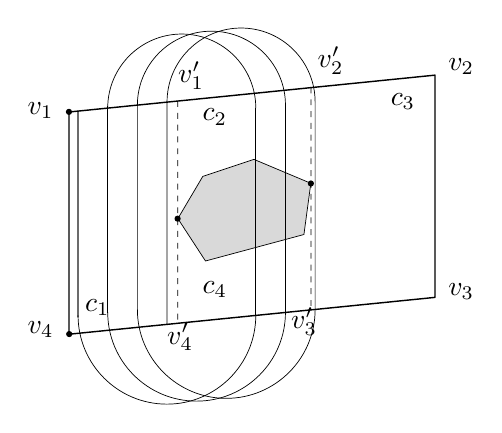
\begin{tikzpicture}[y=0.80pt, x=0.80pt, yscale=-\globalscale, xscale=\globalscale, inner sep=0pt, outer sep=0pt]
\path[draw=black,line join=round,line width=0.512pt] (18.6584,38.0894) -- (183.9870,21.4419) -- (183.9870,121.8210) -- (18.6584,138.4690) -- (18.6584,38.0894) -- cycle;



\path[draw=black,fill=black,line join=round,line width=0.512pt] (18.6440,36.9516) .. controls (19.2323,36.9516) and (19.7092,37.4286) .. (19.7092,38.0169) .. controls (19.7092,38.6052) and (19.2323,39.0821) .. (18.6440,39.0821) .. controls (18.0557,39.0821) and (17.5787,38.6052) .. (17.5787,38.0169) .. controls (17.5787,37.4286) and (18.0557,36.9516) .. (18.6440,36.9516) -- cycle;



\path[draw=black,fill=cD9D9D9,line join=round,line width=0.256pt] (67.8359,86.2298) -- (79.1010,67.1658) -- (102.1880,59.4805) -- (127.8940,70.2900) -- (124.7750,93.4267) -- (80.3210,105.3850) -- (67.8359,86.2298) -- cycle;



\path[draw=black,fill=black,line join=round,line width=0.512pt] (18.7578,137.3230) .. controls (19.3461,137.3230) and (19.8230,137.8000) .. (19.8230,138.3880) .. controls (19.8230,138.9760) and (19.3461,139.4530) .. (18.7578,139.4530) .. controls (18.1695,139.4530) and (17.6925,138.9760) .. (17.6925,138.3880) .. controls (17.6925,137.8000) and (18.1695,137.3230) .. (18.7578,137.3230) -- cycle;



\path[cm={{1.0,0.0,0.0,1.0,(0.0,41.0)}}] (0.0000,0.0000) node[above right] () {$v_1$};



\path[cm={{1.0,0.0,0.0,1.0,(0.0,140.0)}}] (0.0000,0.0000) node[above right] () {$v_4$};



\path[cm={{1.0,0.0,0.0,1.0,(190.0,21.0)}}] (0.0000,0.0000) node[above right] () {$v_2$};



\path[cm={{1.0,0.0,0.0,1.0,(190.0,123.0)}}] (0.0000,0.0000) node[above right] () {$v_3$};



\path[fill=black,line join=round,line width=0.256pt] (67.9514,38.4827) -- (67.9514,41.1494) -- (67.6314,41.1494) -- (67.6314,38.4827) -- (67.9514,38.4827) -- cycle(67.9514,43.8160) -- (67.9514,46.4827) -- (67.6314,46.4827) -- (67.6314,43.8160) -- (67.9514,43.8160) -- cycle(67.9514,49.1494) -- (67.9514,51.8160) -- (67.6314,51.8160) -- (67.6314,49.1494) -- (67.9514,49.1494) -- cycle(67.9514,54.4827) -- (67.9514,57.1494) -- (67.6314,57.1494) -- (67.6314,54.4827) -- (67.9514,54.4827) -- cycle(67.9514,59.8160) -- (67.9514,62.4827) -- (67.6314,62.4827) -- (67.6314,59.8160) -- (67.9514,59.8160) -- cycle(67.9514,65.1494) -- (67.9514,67.8160) -- (67.6314,67.8160) -- (67.6314,65.1494) -- (67.9514,65.1494) -- cycle(67.9514,70.4827) -- (67.9514,73.1494) -- (67.6314,73.1494) -- (67.6314,70.4827) -- (67.9514,70.4827) -- cycle(67.9514,75.8160) -- (67.9514,78.4827) -- (67.6314,78.4827) -- (67.6314,75.8160) -- (67.9514,75.8160) -- cycle(67.9514,81.1494) -- (67.9514,83.8160) -- (67.6314,83.8160) -- (67.6314,81.1494) -- (67.9514,81.1494) -- cycle(67.9514,86.4827) -- (67.9514,89.1494) -- (67.6314,89.1494) -- (67.6314,86.4827) -- (67.9514,86.4827) -- cycle(67.9514,91.8160) -- (67.9514,94.4827) -- (67.6314,94.4827) -- (67.6314,91.8160) -- (67.9514,91.8160) -- cycle(67.9514,97.1494) -- (67.9514,99.8160) -- (67.6314,99.8160) -- (67.6314,97.1494) -- (67.9514,97.1494) -- cycle(67.9514,102.4830) -- (67.9514,105.1490) -- (67.6314,105.1490) -- (67.6314,102.4830) -- (67.9514,102.4830) -- cycle(67.9514,107.8160) -- (67.9514,110.4830) -- (67.6314,110.4830) -- (67.6314,107.8160) -- (67.9514,107.8160) -- cycle(67.9514,113.1490) -- (67.9514,115.8160) -- (67.6314,115.8160) -- (67.6314,113.1490) -- (67.9514,113.1490) -- cycle(67.9514,118.4830) -- (67.9514,121.1490) -- (67.6314,121.1490) -- (67.6314,118.4830) -- (67.9514,118.4830) -- cycle(67.9514,123.8160) -- (67.9514,126.4830) -- (67.6314,126.4830) -- (67.6314,123.8160) -- (67.9514,123.8160) -- cycle(67.9514,129.1490) -- (67.9514,131.8160) -- (67.6314,131.8160) -- (67.6314,129.1490) -- (67.9514,129.1490) -- cycle(67.9514,33.1494) -- (67.9514,35.8160) -- (67.6314,35.8160) -- (67.6314,33.1494) -- (67.9514,33.1494) -- cycle;



\path[draw=black,fill=black,line join=round,line width=0.512pt] (67.7196,85.1953) .. controls (68.3080,85.1953) and (68.7849,85.6723) .. (68.7849,86.2606) .. controls (68.7849,86.8489) and (68.3080,87.3258) .. (67.7196,87.3258) .. controls (67.1313,87.3258) and (66.6544,86.8489) .. (66.6544,86.2606) .. controls (66.6544,85.6723) and (67.1313,85.1953) .. (67.7196,85.1953) -- cycle;



\path[fill=black,line join=round,line width=0.256pt] (128.1570,32.3496) -- (128.1570,35.0162) -- (127.8370,35.0162) -- (127.8370,32.3496) -- (128.1570,32.3496) -- cycle(128.1570,37.6829) -- (128.1570,40.3496) -- (127.8370,40.3496) -- (127.8370,37.6829) -- (128.1570,37.6829) -- cycle(128.1570,43.0162) -- (128.1570,45.6829) -- (127.8370,45.6829) -- (127.8370,43.0162) -- (128.1570,43.0162) -- cycle(128.1570,48.3496) -- (128.1570,51.0162) -- (127.8370,51.0162) -- (127.8370,48.3496) -- (128.1570,48.3496) -- cycle(128.1570,53.6829) -- (128.1570,56.3496) -- (127.8370,56.3496) -- (127.8370,53.6829) -- (128.1570,53.6829) -- cycle(128.1570,59.0162) -- (128.1570,61.6829) -- (127.8370,61.6829) -- (127.8370,59.0162) -- (128.1570,59.0162) -- cycle(128.1570,64.3496) -- (128.1570,67.0162) -- (127.8370,67.0162) -- (127.8370,64.3496) -- (128.1570,64.3496) -- cycle(128.1570,69.6829) -- (128.1570,72.3496) -- (127.8370,72.3496) -- (127.8370,69.6829) -- (128.1570,69.6829) -- cycle(128.1570,75.0162) -- (128.1570,77.6829) -- (127.8370,77.6829) -- (127.8370,75.0162) -- (128.1570,75.0162) -- cycle(128.1570,80.3496) -- (128.1570,83.0162) -- (127.8370,83.0162) -- (127.8370,80.3496) -- (128.1570,80.3496) -- cycle(128.1570,85.6829) -- (128.1570,88.3496) -- (127.8370,88.3496) -- (127.8370,85.6829) -- (128.1570,85.6829) -- cycle(128.1570,91.0162) -- (128.1570,93.6829) -- (127.8370,93.6829) -- (127.8370,91.0162) -- (128.1570,91.0162) -- cycle(128.1570,96.3496) -- (128.1570,99.0162) -- (127.8370,99.0162) -- (127.8370,96.3496) -- (128.1570,96.3496) -- cycle(128.1570,101.6830) -- (128.1570,104.3500) -- (127.8370,104.3500) -- (127.8370,101.6830) -- (128.1570,101.6830) -- cycle(128.1570,107.0160) -- (128.1570,109.6830) -- (127.8370,109.6830) -- (127.8370,107.0160) -- (128.1570,107.0160) -- cycle(128.1570,112.3500) -- (128.1570,115.0160) -- (127.8370,115.0160) -- (127.8370,112.3500) -- (128.1570,112.3500) -- cycle(128.1570,117.6830) -- (128.1570,120.3500) -- (127.8370,120.3500) -- (127.8370,117.6830) -- (128.1570,117.6830) -- cycle(128.1570,123.0160) -- (128.1570,125.6830) -- (127.8370,125.6830) -- (127.8370,123.0160) -- (128.1570,123.0160) -- cycle(128.1570,27.0162) -- (128.1570,29.6829) -- (127.8370,29.6829) -- (127.8370,27.0162) -- (128.1570,27.0162) -- cycle;



\path[draw=black,fill=black,line join=round,line width=0.512pt] (127.9250,69.3134) .. controls (128.5130,69.3134) and (128.9900,69.7904) .. (128.9900,70.3787) .. controls (128.9900,70.9670) and (128.5130,71.4439) .. (127.9250,71.4439) .. controls (127.3370,71.4439) and (126.8600,70.9670) .. (126.8600,70.3787) .. controls (126.8600,69.7904) and (127.3370,69.3134) .. (127.9250,69.3134) -- cycle;



\path[cm={{1.0,0.0,0.0,1.0,(68.0,28.0)}}] (0.0000,0.0000) node[above right] () {$v_1'$};



\path[cm={{1.0,0.0,0.0,1.0,(63.0,146.0)}}] (0.0000,0.0000) node[above right] () {$v_4'$};



\path[cm={{1.0,0.0,0.0,1.0,(131.0,21.0)}}] (0.0000,0.0000) node[above right] () {$v_2'$};



\path[cm={{1.0,0.0,0.0,1.0,(119.0,139.0)}}] (0.0000,0.0000) node[above right] () {$v_3'$};



\path[cm={{1.0,0.0,0.0,1.0,(26.0,130.0)}}] (0.0000,0.0000) node[above right] () {$c_1$};



\path[cm={{1.0,0.0,0.0,1.0,(79.0,44.0)}}] (0.0000,0.0000) node[above right] () {$c_2$};



\path[cm={{1.0,0.0,0.0,1.0,(164.0,37.0)}}] (0.0000,0.0000) node[above right] () {$c_3$};



\path[cm={{1.0,0.0,0.0,1.0,(79.0,122.0)}}] (0.0000,0.0000) node[above right] () {$c_4$};



\path[draw=black,line join=round,line width=0.256pt] (22.7526,37.5564) -- (22.7519,130.8090);



\path[draw=black,line join=round,line width=0.256pt] (36.1519,36.3182) .. controls (36.1519,17.8485) and (51.1257,2.8747) .. (69.5955,2.8747) .. controls (88.0652,2.8747) and (103.0390,17.8485) .. (103.0390,36.3182);



\path[draw=black,line join=round,line width=0.256pt] (103.0390,129.9020) .. controls (103.0390,152.0720) and (85.0663,170.0450) .. (62.8959,170.0450) .. controls (40.7255,170.0450) and (22.7528,152.0720) .. (22.7528,129.9020);



\path[draw=black,line join=round,line width=0.256pt] (103.0390,36.2164) -- (103.0390,114.7450);



\path[draw=black,line join=round,line width=0.256pt] (103.0390,114.6320) -- (103.0390,130.0610);



\path[draw=black,line join=round,line width=0.256pt] (36.1520,35.3868) -- (36.1520,128.7350);



\path[draw=black,line join=round,line width=0.256pt] (49.5513,34.9866) -- (49.5511,127.8360);



\path[draw=black,line join=round,line width=0.256pt] (22.7526,37.5564) -- (22.7519,130.8090);



\path[draw=black,line join=round,line width=0.256pt] (116.4380,34.7485) -- (116.4380,128.5930);



\path[draw=black,line join=round,line width=0.256pt] (116.4380,128.5400) .. controls (116.4380,150.7110) and (98.4656,168.6830) .. (76.2952,168.6830) .. controls (54.1248,168.6830) and (36.1520,150.7110) .. (36.1520,128.5400);



\path[draw=black,line join=round,line width=0.256pt] (49.5512,35.0285) .. controls (49.5512,16.5588) and (64.5251,1.5850) .. (82.9948,1.5850) .. controls (101.4650,1.5850) and (116.4380,16.5588) .. (116.4380,35.0285);



\path[draw=black,line join=round,line width=0.256pt] (129.8380,127.2860) .. controls (129.8380,149.4560) and (111.8650,167.4290) .. (89.6944,167.4290) .. controls (67.5240,167.4290) and (49.5513,149.4560) .. (49.5513,127.2860);



\path[draw=black,line join=round,line width=0.256pt] (129.8370,33.5190) -- (129.8380,127.3630);



\path[draw=black,line join=round,line width=0.256pt] (62.9505,33.6034) .. controls (62.9505,15.1336) and (77.9243,0.1599) .. (96.3940,0.1599) .. controls (114.8640,0.1599) and (129.8380,15.1336) .. (129.8380,33.6034);



\path[draw=black,line join=round,line width=0.256pt] (62.9507,33.8022) -- (62.9504,134.0530);




\end{tikzpicture}


  \caption[The Zamboni-like motion with the lowest parameter configuration.]{The Zamboni-like motion to cover the cell $c_1$ with the lowest configuration of parameter $c_{4,1}$ relative to the radius of the circle $\varphi_4$ in the primitive paths that form the coverage that we introduced in \fref{sec:path-wise}{Section}.}
  \label{fig:zambo2}
\end{figure}
\fref{fig:zambo1}{Figure} showed the coverage of the cell $c_1$ with the highest configuration of parameter $c_{4,1}$. If we assume that the time needed to perform the circle $\varphi_4(\overline{c}_{4,1})$ is $t_3$, the vertical lines $\varphi_1,\varphi_3$ is $2t_1$, and the circle $\varphi_2$ is $t_2$, then the overall time to cover $c_1$ with configuration ${c}_{4,1}=\overline{c}_{4,1}$ is $t_{\overline{c}_{4,1}}=7(2t_1+t_2+t_3)+t_1$. Conversely, in \fref{fig:zambo2}{Figure} we assume that the time needed to perform $\varphi_4(\underline{c}_{4,1})$ is $t_4$; then the time needed to cover $c_1$ with configuration ${c}_{4,1}=\underline{c}_{4,1}$ is $t_{\underline{c}_{4,1}}=3(2t_1+t_2+t_4)+t_1$. It is clear that $t_4<t_3$ (for how the parameter $c_{4,1}$ is constructed in \fref{sec:path-wise}{Section}) and thus $t_{\underline{c}_{4,1}}<t_{\overline{c}_{4,1}}$. If we further assume that traveling all the paths take a similar time $t_1\approx t_2\approx t_3\approx t_4$, then we can observe a 45\% time reduction in flying \fref{fig:zambo2}{Figure} compared to flying \fref{fig:zambo1}{Figure}. Analogously, in the energy domain, we can expect a considerable reduction in the battery drain with ${c}_{4,1}=\underline{c}_{4,1}$ compared to ${c}_{4,1}=\overline{c}_{4,1}$. Our purpose in the remaining of this section is to find the configuration of the path (in the latter case of $c_{4,1}$) along with the computations parameters to maximize the coverage with SoC higher than zero--to find the optimal control on $N$ w.r.t. a given energy cost.

The derivation of such optimal control involves the definition of an OCP\findex{optimal control problem} and its transformation into a nonlinear program (\Gls{acr:nlp})\findex{nonlinear program}~\citep{rawlings2017model,grune2017nonlinear}. Before, however, we re-evaluate the output constraints to include the battery model in \fref{sec:battery-model}{Section}. 
%\subsubsubsection{Output constraint set}
The output of the model in \frefeq{eq:state-perf} is the instantaneous energy consumption $y$ that we stated earlier evolves in $\mathbb{R}$. Nevertheless, there is a limit to the instantaneous energy consumption drainable from a battery at a given time instant. Moreover, aerial robots are bounded by strict energy budgets due to battery limitations, as we motivated in \fref{sec:motivation}{Section}. Hence, we redefine the original output constraint ($\mathbb{R}$) to include the battery model in \fref{sec:battery-model}{Section}. We consider SoC $b$ of the mobile robot's battery with the simplistic differential model in \frefeqM{eq:battery-model-1}{eq:battery-model-2}
\begin{equation}\label{eq:bat}
  \dot{b}(y(t),t)=-k_b\left(V-
  \sqrt{
    V^2-
    4R_ry(t)}
  \right)/(2R_rQ_c),
\end{equation}
where $k_b$ is the battery coefficient determined experimentally,  $V\in\mathbb{R}$ is the internal battery voltage measured in volts, $R_r\in\mathbb{R}$ the resistance measured in ohms, and $Q_c\in\mathbb{R}$ the constant nominal capacity measured in amperes per hour. 

From the literature on the battery SoC~\citep{sunden2019thermal,kurzweil2018state,kurzweil2021state,deng2017maximum}, we know that this latter can be calculated as $b(y(t),t)=Q(y(t),t)/Q_c$ where $Q(y(t),t)$ is the available capacity at a given time $t$. For simplicity, we omit further details that interfere in the calculation, such as battery state of health\findex{state of health}, temperature, and C-rate\findex{C-rate}. Indeed that are other methods in the literature~\citep{lu2013review,zhang2018state,espedal2021current} to estimate more accurately the SoC together with other battery parameters (these are, however, beyond the scopes of our work of coverage planning and scheduling). From the previous expression and the estimated SoC in \frefeq{eq:bat}, we can calculate the maximum instantaneous energy consumption by multiplying the constant nominal capacity, the SoC, and the internal battery voltage. We assume the maximum energy consumption cannot be negative
\begin{equation}
  0\leq y(t)\leq b(y(t),t)Q_cV,
\end{equation}
and therefore, we define a time-varying constraint for the output in \fref{def:const}{Definition}, being the maximum instantaneous energy consumption dependent on the SoC $b$ from \frefeq{eq:bat}, which is dependent on time and the instantaneous energy consumption (at the previous time step).
\begin{highlight}
\begin{defn}[Output constraint]\label{def:const}
\begin{equation*}
  \mathcal{Y}(t):=\{y\mid y\in[0,b(y(t),t)Q_cV]\subseteq{\mathbb{R}_{\geq 0}}\},
\end{equation*}
is the \emph{output constraint}\findex{output constraint}, where $b(y(t),t)Q_cV$ is the maximum instantaneous energy consumption.
\end{defn}
\end{highlight}
We assume the mobile robot carries a battery energy sensor and obtain the initial SoC $b(y(t_0),t_0)$ in the output constraint using the output of such sensor. This is a realistic assumption: aerial robots are often equipped with a flight controller, which returns various metrics, including the battery SoC. Evaluating the constraint requires numerical simulation: the battery model in \frefeq{eq:bat} is differential, similarly to the energy dynamics of the periodic model in \frefeq{eq:state-perf}. We can compute the numerical simulation using the Euler method in \fref{sec:euler}{Section} or the Runge-Kutta method in \fref{sec:rk4}{Section}. 

To state the OCP on a finite horizon, we use a similar expression to \fref{sec:opt-constrained}{Section} with
\begin{subequations}\label{eq:ocp-output-mpc}\begin{align}
  \max_{\mathbf{q}(t),c_i(t)}&{l_f(\mathbf{q}(T),T)+\int_{t_0}^T{l(\mathbf{q}(t),c_i(t),t)\,dt}},\\
  \text{s.t. }\dot{\mathbf{q}}&=f(\mathbf{q}(t),c_i(t),t),\label{eq:dyn-evol}\\
  c_i(t)&\in\mathcal{U}_i,\mathbf{q}(t)\in\mathbb{R}^m,\label{eq:state-cont-const-mpc}\\
  y(t)&\in\mathcal{Y}(t),\label{eq:batt-const-mpc}\\
  \mathcal{S}_{i,j}&:=\{0\},\,\forall j \in [\sigma]\text{ when }\mathbf{p}(t)\notin\mathcal{Q}^v,\label{eq:polyg-const}\\
  \mathbf{q}(t_0)&=\hat{\mathbf{q}}_0\,\,\,\text{given (last estimate state)},\text{ and}\\
  b(y(t_0),t_0)&=b_0\,\,\,\text{given},
\end{align}\end{subequations}
where constraints in \frefeqM{eq:dyn-evol}{eq:polyg-const} are evaluated on $t\in[t_0,T]$. $\mathbf{q}(t)$ and $c_i(t)$ are the state and control trajectories and $\mathbf{p}(t)$ is the aerial robot's position w.r.t. an inertial navigation frame $\mathcal{O}_W$. The sizes of the state and control ($m$ and $n$) are defined in \fref{sec:periodic-model}{Section} and \fref{sec:nom-cont}{Section}. By solving the OCP in \frefeq{eq:ocp-output-mpc}, we want to derive the trajectory $c_i^*(t)=\{c^*_{i,1},\dots,c^*_{i,\rho},c^*_{i,\rho+1},\dots,c^*_{i,\rho+\sigma}\}$ in \fref{sec:defs-stages-triggs}{Section} for a given stage $i$ in \fref{def:stage}{Definition}. In the $\max$ term in \frefeq{eq:ocp-output-mpc}, we further derive the trajectory of the ideal state $\mathbf{q}(t)$, which we can use to evaluate the model's fidelity against future measured data. Indeed the solution to the OCP has to  evolve the model from trained data using state estimation up to the initial time instant $t_0$. At the very beginning of the optimization (when $t_0=0$), we will see that the perfect model evolution in \frefeq{eq:dyn-evol} does not correspond to the data despite converging later on: for successive horizons, there $\exists k\text{ s.t. }t_0=kN$ and the model in \frefeq{eq:dyn-evol} converges for $\mathbf{q}(kN)=\hat{\mathbf{q}}_{kN}$. Our constraints contain the control and state constraint in \frefeq{eq:constraint-set}, the output constraint in \fref{def:const}{Definition}, and the dynamics with the ideal state evolution in \frefeq{eq:state-perf} in \frefeqM{eq:dyn-evol}{eq:batt-const-mpc}. The OCP further contains the coverage constraint from \fref{sec:path-wise}{Section} and \fref{sec:cov-motion}{Section} in \frefeq{eq:polyg-const}. Although the aerial robot can overfly the obstacles and the edges of the polygon, it cannot compute any computation. Formally, we inhibit the computations setting their constraint to $\{0\}$ when the aerial robot is flying over the $i$th obstacle $o_i$ and out of the polygon $v$ (it is thus out of the space $\mathcal{Q}^v$). We have similarly inhibited the computations out of the polygon $v$ in \fref{sec:path-wise}{Section}.

The dynamic evolution in \frefeq{eq:dyn-evol} is then the periodic model in \frefeq{eq:state-perf} together with the scale transformation from \fref{sec:merging}{Section}
\begin{equation}\label{eq:perf-model-in-mpc}
  f(\mathbf{q}(t),c_i(t),t)=A\mathbf{q}(t)+B\mathrm{diag}(\nu_i)(c_i(t)-c_i(t-\Delta t)),
\end{equation}
where $c_i(t-\Delta t)$ is the control at the time instant preceding $t$, $A$ is the state transition matrix in \frefeq{eq:mat_A}, $B$ the input matrix in \frefeq{eq:mat_B}, and $\nu_i$ is the scale transformation in \frefeq{eq:scaling} with the scaling factors that for the first $\rho$ path parameters are given in \frefeq{eq:scale-traj} and for the remaining computations parameters in \frefeq{eq:scale-comp}.

The instantaneous cost function is the quadratic expression
\begin{equation}\label{eq:insta-cost-mpc}
  l(\mathbf{q}(t),c_i(t),t)=\mathbf{q}'(t)Q\mathbf{q}(t)+c_i'(t)Rc_i(t),
\end{equation}
where $Q\in\mathbb{R}^{m\times m},R\in\mathbb{R}^{n\times n}$ are given positive semidefinite matrices, resulting in the convexity of the cost $l$~\citep{nocedal2006numerical} with some guarantees on the solution~\citep{beck2014introduction}.

The final cost function is alike a quadratic expression but with no control
\begin{equation}\label{eq:final-cost-mpc}
  l_f(\mathbf{q}(T),T)=\mathbf{q}'(T)Q_f\mathbf{q}(T),
\end{equation}
where $Q_f\in\mathbb{R}^{m\times m}$ is a given positive semidefinite matrix.

The horizon $N$ is in seconds, and the controller selects the optimal control trajectory $c_i^*(t)$ over $[t_0,T]$, with $T=t_0+N$. At each instant, the controller refines the control trajectory (replans the coverage and schedule) that respects the constraints. To evaluate the state trajectory--needed for the instantaneous cost function $l$ and the final cost function $l_f$--the controller evaluates the battery trajectory $b(y(t),t)$ (it has to verify that the output is in $\mathcal{Y}(t)$). It then maximizes the instantaneous cost function $l$ for all the time instants but $T$ ($t_0\leq t < t_0+N$), and the final cost function $l_f$ in \frefeq{eq:final-cost-mpc} for the time instant $T$ ($t=t_0+N$).
The dynamics constraint satisfaction requires to evolve the perfect model $f$ in \frefeq{eq:perf-model-in-mpc} over horizon $[t_0,t_0+N]$ beginning from the last estimated state $\mathbf{q}_0=\hat{\mathbf{q}}(t_0)$ at time instant $t_0$. Similarly, the output constraint satisfaction requires then to evolve the battery constraint on $[t_0,t_0+N]$, from the last battery measurement $b_0$ from the battery energy sensor at instant $t_0$.

The OCP from \frefeq{eq:ocp-output-mpc} is infinite-dimensional, being the system dynamics in \frefeq{eq:dyn-evol} and the battery dynamics in \frefeq{eq:bat} given in continuous- and not discrete-time. Such an infinite dimensional OCP has an infinite-dimension of constraints and decision variables since there are infinitely many time instants between $t_0$ and $t_0+N$. We discretize the OCP to finite dimensions in \fref{sec:opt-cont-gener}{Section}.

\subsection{Replanning with output model predictive control}
\label{sec:opt-cont-gener}

In this section, we solve the OCP in \frefeq{eq:ocp-output-mpc}, providing a solution to \fref{pb}{Problem} that we introduced along with \fref{pb:cov-pb}{Problem} in \fref{cp:soa}{Chapter}. We use the notions from the previous sections and \fref{cp:model}{Chapters}\fref{cp:opt}{--\hspace*{-.8ex}}: with the solution, we derive the configuration of paths and computations $c_i^*$ for each stage $i$ in an energy-aware fashion to replan the plan $\Gamma$. The solution to \fref{pb:cov-pb}{Problem} is the plan $\Gamma$, which contains the primitive paths for the coverage motion in \fref{sec:cov-motion}{Section} and \fref{sec:path-wise}{Section}, along with the computations in \fref{sec:computation-wise}{Section}. 

We are interested in providing this solution online, with a procedure running onboard the aerial robot subject to various atmospheric interferences. There are different techniques for this purpose~\citep{grune2017nonlinear,rawlings2017model}. In \fref{cp:opt}{Chapter}, we saw some relevant to our approach, which are the direct methods already employed in many MPC-related applications~\citep{rawlings2017model}. In particular, we saw single and multiple shooting methods\findex{single shooting method}\findex{multiple shooting method} in \fref{sec:single-shoot}{Sections}\fref{sec:multi-shoot}{--\hspace*{-.8ex}}. They parametrize the control and state trajectories with a finite-dimensional vector and derive an NLP~\citep{rawlings2017model}. Both the methods perform this latter discretization, but the resulting NLP differs. The multiple shooting method keeps the states as decision variables at the boundary time points, allowing further optimizations~\citep{rawlings2017model}. It combines some of the advantages of the other methods, such as the direct collocation method\findex{collocation method} that we discussed in \fref{sec:colloc}{Section}, together with the direct single shooting method~\citep{diehl2006fast,grune2017nonlinear}. Once we obtain the finite-dimensional NLP, we can solve it numerically, with the numerical solvers available in the literature~\citep{diehl2006fast,grune2017nonlinear,nocedal2006numerical}. 

The NLP derived from the OCP in \frefeq{eq:ocp-output-mpc} is
\begin{subequations}\label{eq:disc-ocp-output-mpc}\begin{align}
  \max_{\mathbf{q}(k),c_i(k)}{l_f(\mathbf{q}(T}&{),T)+\sum_{k\in\mathcal{K}}{l_d(\mathbf{q}(k),c_i(k),k)}},\\
  \text{s.t. }\mathbf{q}(k+h)&=f_d(\mathbf{q}(k),c_i(k),k),\label{eq:disc-dyn-evol}\\
  c_i(k)&\in\mathcal{U}_i,\mathbf{q}(k)\in\mathbb{R}^m,\label{eq:disc-state-cont-const-mpc}\\
  y(k)&\in\mathcal{Y}(k),\label{eq:disc-batt-const-mpc}\\
  \mathcal{S}_{i,j}&:=\{0\},\,\forall j \in [\sigma]\text{ when }\mathbf{p}(k)\notin\mathcal{Q}^v,\label{eq:disc-polyg-const}\\
  \mathbf{q}(t_0)&=\hat{\mathbf{q}}_0\,\,\,\text{given (last estimated state)},\text{ and}\\
  b(y(t_0),t_0)&=b_0\,\,\,\text{given},
\end{align}\end{subequations}
where the constraints in \frefeqM{eq:disc-dyn-evol}{eq:disc-polyg-const} are evaluated now on a finite interval $k\in\mathcal{K}=\{t_0,t_0+h,t_0+2h,\dots,T\}$, and $h$ is a given time step or distance between two  consecutive time instants; the smaller the distance, the more precise the simulation. The other expressions are analogous to \frefeq{eq:ocp-output-mpc}.

We use numerical simulation\findex{numerical simulation} to transform \frefeq{eq:ocp-output-mpc} into \frefeq{eq:disc-ocp-output-mpc}. We can use either the Runge-Kutta methods\findex{Runge-Kutta methods} in \fref{sec:rk4}{Section} or the Euler method\findex{Euler method} in \fref{sec:euler}{Section}. For simplicity, we show the transformation with the Euler method. The instantaneous cost function
\begin{equation}\label{eq:mpc-cost-euler}
  l_d(\mathbf{q}(k),c_i(k),k)=hl(\mathbf{q}(k),c_i(k),k),
\end{equation}
where $l$ is given in \frefeq{eq:insta-cost-mpc}.

The discrete dynamic evolution in \frefeq{eq:disc-dyn-evol}
\begin{equation}
  f_d(\mathbf{q}(k),c_i(k),k)=A_d\mathbf{q}(k)+B\mathrm{diag}(\nu_i)(c_i(k)-c_i(k-h)),
\end{equation}
where $A_d$ is the discretized version of the state transition matrix $A$ in \frefeq{eq:mat_A} and for a small enough interval of $h$
\begin{equation}
A_d=(hA+\mathrm{diag}(1,1,\dots,1)),
\end{equation}
where $\mathrm{diag}(1,1,\dots,1)\in\mathbb{R}^{m\times m}$ is a diagonal matrix of ones. $B$ is then the input matrix in \frefeq{eq:mat_B}, and $\nu_i$ is the scale transformation in \frefeq{eq:scaling} with the scaling factors that for the first $\rho$ path parameters are given in \frefeq{eq:scale-traj} and for the remaining $\sigma$ computations parameters in \frefeq{eq:scale-comp}, similarly to \frefeq{eq:perf-model-in-mpc}.

To discretize the battery dynamics in \frefeq{eq:bat}, we use
\begin{equation}\label{eq:batt-euler}
  b_d(y(k+h),k+h)=b(y(k),k)+hb(y(k+h),k+h),
\end{equation}
where $b$ is given in \frefeq{eq:bat} and $y(k)$ is the output of the model in \frefeq{eq:state-perf-output}. The matrix $C$ is to be found in \frefeq{eq:mat_C}.

In \frefeq{eq:disc-ocp-output-mpc}, we transformed the OCP in \frefeq{eq:ocp-output-mpc} into an NLP by first discretizing and thus effectively implementing the direct multiple shooting method in \fref{sec:multi-shoot}{Section}. We note that we can implement the single shooting method by keeping only the initial state as the decision variable $\hat{\mathbf{q}}_0$, conversely to using the interval boundary time points as a decision variable in the multiple shooting method~\citep{rawlings2017model}.

\subsection{Coverage planning and scheduling algorithm}
\label{sec:algo}

\fref{algo:repla}{Algorithm} derives the optimal configuration of path and computations parameters and thus computes the coverage (re)planning and scheduling. It inputs the initial plan $\Gamma$ along with the initial time step and a guess for the energy model that we proposed in \fref{sec:period-est}{Section} and outputs the revised plan $\Gamma$ when the aerial robot reaches the final point $\mathbf{p}_{\Gamma_l}$. It optionally inputs then the initial stage that is within $[n]_{>0}$ when $\Gamma$ compromise primitive stages, $[l]_{>0}$ otherwise. In the remainder of this chapter, we discuss in detail the algorithm.

\begin{algorithm}[h!] %this is an example
  \SetKwInOut{Input}{Input}
  \SetKwInOut{Output}{Output}
  \SetKwFunction{FMain}{\small\tt zamboni-like\_motion}
  \SetKwProg{Fn}{Function}{:}{}
  \SetKwProg{Pn}{Function}{:}{\KwRet}

  \DontPrintSemicolon
  \Input{$\Gamma${ \otherfont initial plan}\newline
         $t_0${ \otherfont initial time step}\newline
         $\mathbf{q}(t_0)${ \otherfont initial guess for the energy model}\newline
         $j${ \otherfont starting stage within the primitive stages }$\in[n]_{>0}${ \otherfont otherwise }$j=1$
  }
  \Output{$\Gamma${ \otherfont revised plan}
  }
  \vspace{.8ex}

  %{\normalsize $j\gets 1$}\;
  
  \ForEach{\normalsize $i\in\{t_0,t_0+h,t_0+2h,\dots\}$}{\label{algo:repla:foreach}
    \If{\normalsize $\mathbf{p}(i)\neq\mathbf{p}_{\Gamma_l}$}{\label{algo:repla:endcheck}
      \Return{\normalfont $\Gamma$}\;\label{algo:repla:return}
    }
    \If{\normalsize $\mathbf{p}(i)=\mathbf{p}_{\Gamma_j}$}{\label{algo:repla:istrig}
      {\normalsize $j\gets j+1$}\;
      \If{\normalsize $j\notin[n]_{>0}$}{
        {\normalsize $j\gets 1$}\;
        {\normalsize $\varphi_1,\varphi_2,\dots,\varphi_n\gets${ \otherfont shift }$\varphi_1,\varphi_2,\dots,\varphi_n${ \otherfont of }$\mathbf{d}$}\;\label{algo:repla:shiftpaths}
        {\normalsize $\mathbf{p}_{\Gamma_1},\mathbf{p}_{\Gamma_2},\dots,\mathbf{p}_{\Gamma_n}\gets${ \otherfont shift also }$\mathbf{p}_{\Gamma_1},\mathbf{p}_{\Gamma_2},\dots,\mathbf{p}_{\Gamma_n}${ \otherfont of }$\mathbf{d}$}\;\label{algo:repla:shifttrigs}
      }
    }
    \vspace{.8ex}
    
    {\normalsize $\mathbf{q}(\mathcal{K}\setminus\{i+N\}),c_j(\mathcal{K})\gets${ \otherfont solve NLP }$\argmax_{\mathbf{q}(k),c_j(k)}{l_f(\mathbf{q}(i+N),i+N)}+$ \hspace*{1em}${\sum_{k\in\mathcal{K}}{l_d(\mathbf{q}(k),c_j(k),k)}}${ \otherfont from \frefeq{eq:disc-ocp-output-mpc} on }$\mathcal{K}=\{i,i+h,\dots,i+N\}$
    }\;\label{algo:repla:mpc}
    \vspace{.8ex}

    {\normalsize $\mathbf{q}(i+h)\gets A_d\mathbf{q}(i)+B\mathrm{diag}{(\nu_j)}(c_j(i)-c_j(i-h))$}\;\label{algo:repla:sysevo}
    {\normalsize $P(i+h)^-\gets A_d P(i)A_d'+S(i)$}\;\label{algo:repla:covesterrorpri}
    {\normalsize $K(i+h)\gets (P(i+h)^-C')/(CP(i+h)^-C'+V(i))$}\;\label{algo:repla:goodoldkalmygains}
    {\normalsize $\hat{\mathbf{q}}(i+h)\gets${ \otherfont compute }$\mathbf{q}(i+h)+K(i+h)(y(i)-C\mathbf{q}(i+h))${ \otherfont from energy sensor }$y(i)$}\;\label{algo:repla:apoststate}
    {\normalsize $\hat{y}(i+h)+C\hat{\mathbf{q}}(i+h)$}\;
    {\normalsize $P(i+h)\gets (I+K(i+h)C)P(i+h)^-$}\;\label{algo:repla:endkalmy}
    \vspace{.8ex}
    
    {\normalsize $k\gets i$}\;\label{algo:repla:initbat}
    \While{\normalsize $b_d(k)>0$}{
      \If{\normalsize $k\notin\mathcal{K}$}{
        {\normalsize $\mathbf{q}(k+h)\gets A_d\mathbf{q}(k)$}\;\label{algo:repla:sysevobatt}
      }
      {\normalsize $b_d(k+h)\gets b_d(k)-hk_b\left(V-\sqrt{V^2-4R_rC\mathbf{q}(k+h)}\right)/(2R_rQ_c)$}\;\label{algo:repla:battevo}
      {\normalsize $k\gets k+h$}\;
    }
    {\normalsize $t_b\gets k-i$}\;\label{algo:repla:endbat}%the maximum estimated battery time
    {\normalsize $t_s\gets(\mathrm{diag}(\nu_j^\rho)c_j^\rho(i)+\tau_j^\rho)[\overbrace{\begin{matrix}1&1&\cdots&1\end{matrix}}^{\rho}]$}\;\label{algo:repla:configtime}%time needed to do the configuration $c_j(i)$
    {\normalsize $t_r\gets(t_s/\overline{t})(\overline{t}-ih)$}\label{algo:repla:loosingmyreligiontime}\;%remaining time
    \If{\normalsize $t_r<t_b$}{
      {\normalsize $c_j^{\rho}(i)\gets${ \otherfont find }$c_j^{\rho}${ \otherfont with }$t_c\in[0,t_b]${\otherfont , otherwise take }$\underline{c}_j^\rho$}\;\label{algo:repla:newpathparam}
    }
    \vspace{.8ex}
    
    {\normalsize $\mathbf{p}(i+h)\gets${ \otherfont compute from position }$\mathbf{p}(i)${\otherfont , velocity }\normalfont $v(i)${ \otherfont with }\normalfont $\Delta_d\varphi_j${ \otherfont in \fref{algo:track}{Algorith}}}\;\label{algo:repla:gvf}
  }
  \vspace{1.6ex}

  \caption{Coverage (re)planning and scheduling algorithm}
  \label{algo:repla}
\end{algorithm}

The algorithm iterates at each time step $h\in\mathbb{R}_{>0}$ on \fref{algo:repla:foreach}{Line}, with the size of $h$ related to the accuracy and the time needed for replanning: the higher the step, the lower the accuracy, but the shorter the necessary time to replan $\Gamma$. Nonetheless, there are further constraints on $h$ due to the numerical simulation algorithm: $h$ has to be small enough ($h\rightarrow 0$) so that the numerical simulation (on \fref{algo:repla:mpc}{Line}, \fref{algo:repla:sysevo}{}, \fref{algo:repla:sysevobatt}{}, and \fref{algo:repla:battevo}{}) does not diverge. To this end, a typical value for $h$ that we adopted is 1/100 of a second; there are various techniques to estimate $h$ more accurately, e.g., by running the numerical simulation and analyzing the error of two different guesses~\citep{iserles2009first}; such techniques are, however, beyond the scopes of this work. With a small enough $h$, Euler method\findex{Euler method} that we use in \frefeqM{eq:mpc-cost-euler}{eq:batt-euler} converges to the real solution--see~\citep{iserles2009first,atkinson2009euler} for a formal proof--whereas for problems with higher accuracy we advise the Runge-Kutta methods\findex{Runge-Kutta methods}  in \fref{sec:rk4}{Section} that are among the most popular methods for numerical simulation~\citep{atkinson2009euler}. These methods use quadrature\findex{quadrature}: a procedure that replaces the integral with a finite sum~\citep{iserles2009first}. We use the Runge-Kutta inside \powprof{} in \fref{sec:powprof}{Section} and the Euler method in the algorithm for simplicity.

On  \fref{algo:repla:endcheck}{Lines}\fref{algo:repla:return}{--\hspace*{-.8ex}}, the algorithm verifies whenever the aerial robot reached the final point $\mathbf{p}_{\Gamma_l}$ in \fref{def:trigs}{Definition} and returns the replanned plan $\Gamma$ in this latter eventuality, and on \fref{algo:repla:istrig}{Lines}\fref{algo:repla:shifttrigs}{--\hspace*{-.8ex}}, switches the stages when the aerial robot reaches a triggering point (also in \fref{def:trigs}{Definition}). If $\Gamma$ contains $n$ primitive paths rather than all the stages up to $l$ explicitly, on \fref{algo:repla:shiftpaths}{Lines}\fref{algo:repla:shifttrigs}{--\hspace*{-.8ex}}, it updates the paths and the triggering points with the shift $\mathbf{d}$. It then selects the energy-aware configuration of computations on \fref{algo:repla:mpc}{Line} by solving the NLP in \frefeq{eq:disc-ocp-output-mpc} derived from the OCP in \frefeq{eq:ocp-output-mpc} using the multiple shooting method\findex{multiple shooting method} in \fref{sec:multi-shoot}{Section}. It thus obtains the trajectory of the controls and states for a given horizon $N$ expressed in seconds. In particular, the control trajectory contains $|\mathcal{K}|-1$ items, whereas the state trajectory $|\mathcal{K}|$ items. This discrepancy in the number of sets of the two trajectories is due to the construction of OCP. We provide an initial guess for the state $\mathbf{q}(i)$ at time instant $i$ but derive the first control $c_j(i)$ already from the solution to the OCP. For the horizon $N$, we adopted the value of $N$ equal to ten seconds, meaning the algorithm evolves the model in \frefeq{eq:perf-model-in-mpc} and \frefeq{eq:state-perf} for ten future seconds and selects the control trajectory $c_j^*$ that minimizes the costs in \frefeq{eq:mpc-cost-euler} and \frefeq{eq:final-cost-mpc}. The higher the horizon, the better the accuracy. A typical value in the aerial robotics literature that implements MPC~\citep{gavilan2015iterative,kang2009linear,stastny2018nonlinear,chao2011collision} is of dozens of seconds. For instance, it is fourteen in Gavilan~et~al., ten and forty in Kang~and~Hedrick, two to eight in Stastny~and~Siegwart, and five in Chao~et~al.
To solve the NLP in \frefeq{eq:disc-ocp-output-mpc}, the algorithm evaluates the constraints in \frefeqM{eq:disc-dyn-evol}{eq:disc-polyg-const} ($t_0$ in the latest two constraints is equal to $i$), where it has to numerically simulate both the energy and the battery models from $i$ to $i+N$ with a step size of $h$. A possible optimization that considerably speeds up the derivation of the optimal control is to use different horizons for numerical simulation and the constraints, i.e., $\mathcal{H}={i,i+nh,i+2h,i+N}$, where $n\in[1,1/h]$. When $n$ is equal to $1/h$, the algorithm adds the constraints at each second but numerically simulates the models on $\mathcal{K}$. Another optimization is to move the constraint in \frefeq{eq:disc-polyg-const} out of the NLP and check whenever the aerial robot is flying the obstacle and thus require $c_j^\rho={0}$.

On \fref{algo:repla:sysevo}{Lines}\fref{algo:repla:endkalmy}{--\hspace*{-.8ex}}, the algorithm estimates the state $\mathbf{q}$ of the periodic model in \fref{sec:periodic-model}{Section}, filtering the state with Kalman filter in \fref{sec:kalmy}{Section} from the energy sensor's measurements $y(i)$. The Kalman filter\findex{Kalman filter} has several important properties over other methods for state estimation, and among the others, minimizes the variance of the estimation mean square error (\Gls{acr:mse})~\citep{kalman1960new,simon2006optimal,jwo2007practical}. On \fref{algo:repla:sysevo}{Line}, the algorithm computes the a priori, and on \fref{algo:repla:apoststate}{Line} the a posteriori state estimation. On \fref{algo:repla:covesterrorpri}{Line}, the a priori covariance state error with $P$ the covariance of the state estimation error (we provide an initial guess $P(t_0)\in\mathbb{R}^{m\times m}$, the covariance error of $\mathbf{q}(t_0)$) and $S\in\mathbb{R}^{m\times m}$ the covariance of the state noise, and on \fref{algo:repla:goodoldkalmygains}{Line}, the gain with $V\in\mathbb{R}$ the covariance of the output noise~\citep{simon2006optimal}. To ease the computations, we keep the covariances fixed in our experimental setup.

On \fref{algo:repla:initbat}{Lines}\fref{algo:repla:endbat}{--\hspace*{-.8ex}}, the algorithm estimates the time needed to completely drain the battery with the differential model in \fref{sec:battery-model}{Section}, in \frefeq{eq:bat}, and \frefeq{eq:batt-euler}, using the Euler method for numerical simulation (as on \fref{algo:repla:sysevo}{Line}). A possible optimization in this set of lines is to utilize the state already from MPC on \fref{algo:repla:mpc}{Line} for future energy prediction on the horizon $N$; at further time horizons, we don't have any trajectory for the control available, and thus we keep $c_j(k)=c_j(i+N-h),\,\forall k>i+N-h$. The variable $t_b$ on \fref{algo:repla:endbat}{Line} contains the estimated available battery time. The algorithm then computes the scale transformation from the path parameters domain to the time domain in \fref{sec:merging}{Section} on \fref{algo:repla:configtime}{Line} and the estimated remaining time of the path parameters $c_j^\rho(i)$ on \fref{algo:repla:loosingmyreligiontime}{Line}. It selects a different configuration of path parameters when the battery time is lower than the remaining time on \fref{algo:repla:newpathparam}{Line}. We can further assume that the battery information is incomplete or that the model does not account for all the eventualities and select the best configuration for the current total battery time. Finally, on \fref{algo:repla:gvf}{Line}, the algorithm computes the next position in space using the vector field for guidance in \fref{sec:gvf}{Section}, where $v(i)\in\mathbb{R}_{\geq 0}$ is the velocity and $\mathbf{p}(i)$ the position at the current time step $i$. 


%%%%%%%%%%%%%%%%%%%%%%%%%%%%
\section{\color{red}Results}


%%%%%%%%%%%%%%%%%%%%%%%%%%%%
\section{\color{red}Summary}

